% Options for packages loaded elsewhere
\PassOptionsToPackage{unicode}{hyperref}
\PassOptionsToPackage{hyphens}{url}
%
\documentclass[
]{book}
\usepackage{amsmath,amssymb}
\usepackage{lmodern}
\usepackage{iftex}
\ifPDFTeX
  \usepackage[T1]{fontenc}
  \usepackage[utf8]{inputenc}
  \usepackage{textcomp} % provide euro and other symbols
\else % if luatex or xetex
  \usepackage{unicode-math}
  \defaultfontfeatures{Scale=MatchLowercase}
  \defaultfontfeatures[\rmfamily]{Ligatures=TeX,Scale=1}
\fi
% Use upquote if available, for straight quotes in verbatim environments
\IfFileExists{upquote.sty}{\usepackage{upquote}}{}
\IfFileExists{microtype.sty}{% use microtype if available
  \usepackage[]{microtype}
  \UseMicrotypeSet[protrusion]{basicmath} % disable protrusion for tt fonts
}{}
\makeatletter
\@ifundefined{KOMAClassName}{% if non-KOMA class
  \IfFileExists{parskip.sty}{%
    \usepackage{parskip}
  }{% else
    \setlength{\parindent}{0pt}
    \setlength{\parskip}{6pt plus 2pt minus 1pt}}
}{% if KOMA class
  \KOMAoptions{parskip=half}}
\makeatother
\usepackage{xcolor}
\IfFileExists{xurl.sty}{\usepackage{xurl}}{} % add URL line breaks if available
\IfFileExists{bookmark.sty}{\usepackage{bookmark}}{\usepackage{hyperref}}
\hypersetup{
  pdftitle={Formeln Statistik},
  pdfauthor={Lukas Stammler},
  hidelinks,
  pdfcreator={LaTeX via pandoc}}
\urlstyle{same} % disable monospaced font for URLs
\usepackage{color}
\usepackage{fancyvrb}
\newcommand{\VerbBar}{|}
\newcommand{\VERB}{\Verb[commandchars=\\\{\}]}
\DefineVerbatimEnvironment{Highlighting}{Verbatim}{commandchars=\\\{\}}
% Add ',fontsize=\small' for more characters per line
\usepackage{framed}
\definecolor{shadecolor}{RGB}{248,248,248}
\newenvironment{Shaded}{\begin{snugshade}}{\end{snugshade}}
\newcommand{\AlertTok}[1]{\textcolor[rgb]{0.94,0.16,0.16}{#1}}
\newcommand{\AnnotationTok}[1]{\textcolor[rgb]{0.56,0.35,0.01}{\textbf{\textit{#1}}}}
\newcommand{\AttributeTok}[1]{\textcolor[rgb]{0.77,0.63,0.00}{#1}}
\newcommand{\BaseNTok}[1]{\textcolor[rgb]{0.00,0.00,0.81}{#1}}
\newcommand{\BuiltInTok}[1]{#1}
\newcommand{\CharTok}[1]{\textcolor[rgb]{0.31,0.60,0.02}{#1}}
\newcommand{\CommentTok}[1]{\textcolor[rgb]{0.56,0.35,0.01}{\textit{#1}}}
\newcommand{\CommentVarTok}[1]{\textcolor[rgb]{0.56,0.35,0.01}{\textbf{\textit{#1}}}}
\newcommand{\ConstantTok}[1]{\textcolor[rgb]{0.00,0.00,0.00}{#1}}
\newcommand{\ControlFlowTok}[1]{\textcolor[rgb]{0.13,0.29,0.53}{\textbf{#1}}}
\newcommand{\DataTypeTok}[1]{\textcolor[rgb]{0.13,0.29,0.53}{#1}}
\newcommand{\DecValTok}[1]{\textcolor[rgb]{0.00,0.00,0.81}{#1}}
\newcommand{\DocumentationTok}[1]{\textcolor[rgb]{0.56,0.35,0.01}{\textbf{\textit{#1}}}}
\newcommand{\ErrorTok}[1]{\textcolor[rgb]{0.64,0.00,0.00}{\textbf{#1}}}
\newcommand{\ExtensionTok}[1]{#1}
\newcommand{\FloatTok}[1]{\textcolor[rgb]{0.00,0.00,0.81}{#1}}
\newcommand{\FunctionTok}[1]{\textcolor[rgb]{0.00,0.00,0.00}{#1}}
\newcommand{\ImportTok}[1]{#1}
\newcommand{\InformationTok}[1]{\textcolor[rgb]{0.56,0.35,0.01}{\textbf{\textit{#1}}}}
\newcommand{\KeywordTok}[1]{\textcolor[rgb]{0.13,0.29,0.53}{\textbf{#1}}}
\newcommand{\NormalTok}[1]{#1}
\newcommand{\OperatorTok}[1]{\textcolor[rgb]{0.81,0.36,0.00}{\textbf{#1}}}
\newcommand{\OtherTok}[1]{\textcolor[rgb]{0.56,0.35,0.01}{#1}}
\newcommand{\PreprocessorTok}[1]{\textcolor[rgb]{0.56,0.35,0.01}{\textit{#1}}}
\newcommand{\RegionMarkerTok}[1]{#1}
\newcommand{\SpecialCharTok}[1]{\textcolor[rgb]{0.00,0.00,0.00}{#1}}
\newcommand{\SpecialStringTok}[1]{\textcolor[rgb]{0.31,0.60,0.02}{#1}}
\newcommand{\StringTok}[1]{\textcolor[rgb]{0.31,0.60,0.02}{#1}}
\newcommand{\VariableTok}[1]{\textcolor[rgb]{0.00,0.00,0.00}{#1}}
\newcommand{\VerbatimStringTok}[1]{\textcolor[rgb]{0.31,0.60,0.02}{#1}}
\newcommand{\WarningTok}[1]{\textcolor[rgb]{0.56,0.35,0.01}{\textbf{\textit{#1}}}}
\usepackage{longtable,booktabs,array}
\usepackage{calc} % for calculating minipage widths
% Correct order of tables after \paragraph or \subparagraph
\usepackage{etoolbox}
\makeatletter
\patchcmd\longtable{\par}{\if@noskipsec\mbox{}\fi\par}{}{}
\makeatother
% Allow footnotes in longtable head/foot
\IfFileExists{footnotehyper.sty}{\usepackage{footnotehyper}}{\usepackage{footnote}}
\makesavenoteenv{longtable}
\usepackage{graphicx}
\makeatletter
\def\maxwidth{\ifdim\Gin@nat@width>\linewidth\linewidth\else\Gin@nat@width\fi}
\def\maxheight{\ifdim\Gin@nat@height>\textheight\textheight\else\Gin@nat@height\fi}
\makeatother
% Scale images if necessary, so that they will not overflow the page
% margins by default, and it is still possible to overwrite the defaults
% using explicit options in \includegraphics[width, height, ...]{}
\setkeys{Gin}{width=\maxwidth,height=\maxheight,keepaspectratio}
% Set default figure placement to htbp
\makeatletter
\def\fps@figure{htbp}
\makeatother
\setlength{\emergencystretch}{3em} % prevent overfull lines
\providecommand{\tightlist}{%
  \setlength{\itemsep}{0pt}\setlength{\parskip}{0pt}}
\setcounter{secnumdepth}{5}
\usepackage{booktabs}
\usepackage{amsthm}
\makeatletter
\def\thm@space@setup{%
  \thm@preskip=8pt plus 2pt minus 4pt
  \thm@postskip=\thm@preskip
}
\makeatother
\usepackage{booktabs}
\usepackage{longtable}
\usepackage{array}
\usepackage{multirow}
\usepackage{wrapfig}
\usepackage{float}
\usepackage{colortbl}
\usepackage{pdflscape}
\usepackage{tabu}
\usepackage{threeparttable}
\usepackage{threeparttablex}
\usepackage[normalem]{ulem}
\usepackage{makecell}
\usepackage{xcolor}
\ifLuaTeX
  \usepackage{selnolig}  % disable illegal ligatures
\fi
\usepackage[]{natbib}
\bibliographystyle{apalike}

\title{Formeln Statistik}
\author{Lukas Stammler}
\date{2022-03-16}

\begin{document}
\maketitle

{
\setcounter{tocdepth}{1}
\tableofcontents
}
\hypertarget{vorbemerkung}{%
\chapter{Vorbemerkung}\label{vorbemerkung}}

Dieses Dokument fasst die wichtigsten Definitionen und Formeln für Studierende, die an einem Grundkurs Statistik teilnehmen, zusammen. Die Zusammenstellung basiert auf dem Dokument \href{https://rpubs.com/stammler/851041}{Grundkurs Statstik: Formeln und R-Funktionen}, das über Rpubs publiziert wird.
Die Formeln werden durch Beispiele in \texttt{R} ergänzt, um ihre Anwendung zu illustrieren und in die Statistiksoftware einzuführen. Die laufende Erweiterung der ursprünglichen Formelsammlung hat mich zur Neugestaltung als Buch bewegt, da dieses Format leichter zu überarbeiten ist.

Wie immer bin ich dankbar für Kommentare, Ergänzungen und Hinweise auf Fehler an \href{mailto:lukas.stammler@bfh.ch}{\nolinkurl{lukas.stammler@bfh.ch}}.

Frühjahr 2022\\
Lukas Stammler

\hypertarget{Deskriptive}{%
\chapter{Deskriptive Statistik}\label{Deskriptive}}

\hypertarget{kennzahlen-der-zentralen-tendenz-und-der-streuung}{%
\section{Kennzahlen der zentralen Tendenz und der Streuung}\label{kennzahlen-der-zentralen-tendenz-und-der-streuung}}

\hypertarget{umfang}{%
\subsection{Umfang}\label{umfang}}

\(n\) = Stichprobenumfang\\
\(N\) = Umfang der Population

\hypertarget{arithmetisches-mittel-mittelwert}{%
\subsection{Arithmetisches Mittel, Mittelwert}\label{arithmetisches-mittel-mittelwert}}

\(\bar{x}\) = Stichprobenmittelwert\\
\(\mu\) = Populationsmittelwert

\begin{equation}
  \bar{x} = \frac{\sum_{i=1}^n x_i}{n}
  \label{eq:mittelwert}
\end{equation}

mit

\(x_j:\) Messwert der i-ten Beobachtungseinheit in der Stichprobe\\
\(n:\) Anzahl der Beobachtungseinheiten

\begin{Shaded}
\begin{Highlighting}[]
\NormalTok{x }\OtherTok{\textless{}{-}} \FunctionTok{c}\NormalTok{(}\DecValTok{2}\NormalTok{, }\DecValTok{3}\NormalTok{, }\DecValTok{4}\NormalTok{, }\DecValTok{4}\NormalTok{, }\DecValTok{5}\NormalTok{, }\DecValTok{6}\NormalTok{)    }\CommentTok{\# Beispieldaten in Variable x speichern}
\NormalTok{n }\OtherTok{\textless{}{-}} \FunctionTok{length}\NormalTok{(x)              }\CommentTok{\# Anzahl Beobachtungseinheiten n}
\FunctionTok{sum}\NormalTok{(x)}\SpecialCharTok{/}\NormalTok{n                    }\CommentTok{\# Mittelwert berechnen}
\end{Highlighting}
\end{Shaded}

\begin{verbatim}
## [1] 4
\end{verbatim}

\begin{Shaded}
\begin{Highlighting}[]
\FunctionTok{mean}\NormalTok{(x)                     }\CommentTok{\# R{-}Funktion}
\end{Highlighting}
\end{Shaded}

\begin{verbatim}
## [1] 4
\end{verbatim}

\hypertarget{median}{%
\subsection{Median}\label{median}}

wenn \(n\) ungerade

\begin{equation}
  \tilde{x} = x_{\frac{n+1}{2}}
  \label{eq:median1}
\end{equation}

wenn \(n\) gerade

\begin{equation}
  \tilde{x} = \frac{1}{2}(x_{\frac{n}{2}} + {x_{\frac{n}{2}+1}})
  \label{eq:median2}
\end{equation}

Beispiel:

\begin{Shaded}
\begin{Highlighting}[]
\NormalTok{x }\OtherTok{\textless{}{-}} \FunctionTok{c}\NormalTok{(}\DecValTok{2}\NormalTok{, }\DecValTok{3}\NormalTok{, }\DecValTok{4}\NormalTok{, }\DecValTok{4}\NormalTok{, }\DecValTok{5}\NormalTok{, }\DecValTok{6}\NormalTok{, }\DecValTok{10}\NormalTok{)  }\CommentTok{\# Beispieldaten in Variable x speichern}
\FunctionTok{median}\NormalTok{(x)                     }\CommentTok{\# R{-}Funktion}
\end{Highlighting}
\end{Shaded}

\begin{verbatim}
## [1] 4
\end{verbatim}

\hypertarget{varianz}{%
\subsection{Varianz}\label{varianz}}

\(s^2\) = Stichprobenvarianz\\
\(\sigma^2\) = Varianz der Population

Berechnung der Varianz in der Stichprobe zur Schätzung der Populationsvarianz

\begin{equation}
  s^2 = \frac{\sum_{i=1}^n (x_i - \bar{x})^2}{n-1}
  \label{eq:varsample}
\end{equation}

Berechnung der Varianz in der Population

\begin{equation}
  \sigma^2 = \frac{\sum_{i=1}^n (x_i - \mu)^2}{n}
  \label{eq:varpop}
\end{equation}

\begin{Shaded}
\begin{Highlighting}[]
\NormalTok{x }\OtherTok{\textless{}{-}} \FunctionTok{c}\NormalTok{(}\DecValTok{2}\NormalTok{, }\DecValTok{3}\NormalTok{, }\DecValTok{4}\NormalTok{, }\DecValTok{4}\NormalTok{, }\DecValTok{5}\NormalTok{, }\DecValTok{6}\NormalTok{, }\DecValTok{10}\NormalTok{)      }\CommentTok{\# Beispieldaten für eine Stichprobe}
\NormalTok{n }\OtherTok{\textless{}{-}} \FunctionTok{length}\NormalTok{(x)                    }\CommentTok{\# Stichprobenumfang n }
\NormalTok{m }\OtherTok{\textless{}{-}} \FunctionTok{mean}\NormalTok{(x)                      }\CommentTok{\# Mittelwert von x berechnen}
\FunctionTok{sum}\NormalTok{((x }\SpecialCharTok{{-}}\NormalTok{ m)}\SpecialCharTok{\^{}}\DecValTok{2}\NormalTok{)}\SpecialCharTok{/}\NormalTok{(n }\SpecialCharTok{{-}} \DecValTok{1}\NormalTok{)            }\CommentTok{\# Varianz berechnen}
\end{Highlighting}
\end{Shaded}

\begin{verbatim}
## [1] 6.809524
\end{verbatim}

\begin{Shaded}
\begin{Highlighting}[]
\FunctionTok{var}\NormalTok{(x)                            }\CommentTok{\# R{-}Funktion}
\end{Highlighting}
\end{Shaded}

\begin{verbatim}
## [1] 6.809524
\end{verbatim}

\hypertarget{standardabweichung}{%
\subsection{Standardabweichung}\label{standardabweichung}}

\(s\) = Standardabweichung der Stichprobe\\
\(\sigma\) = Standardabweichung der Population

Berechnung der Standardabweichung für eine Stichprobe

\begin{equation}
  s = \sqrt{s^2} = \sqrt{\frac{\sum_{i=1}^n (x_i - \bar{x})^2}{n-1}}
  \label{eq:ssample}
\end{equation}

Berechnung der Standardabweichung für eine Population

\begin{equation}
  \sigma = \sqrt{\sigma^2} = \sqrt{\frac{\sum_{i=1}^n (x_i - \mu)^2}{n}}
  (\\#eq:spop)
\end{equation}

\begin{Shaded}
\begin{Highlighting}[]
\NormalTok{x }\OtherTok{\textless{}{-}} \FunctionTok{c}\NormalTok{(}\DecValTok{2}\NormalTok{, }\DecValTok{3}\NormalTok{, }\DecValTok{4}\NormalTok{, }\DecValTok{4}\NormalTok{, }\DecValTok{5}\NormalTok{, }\DecValTok{6}\NormalTok{, }\DecValTok{10}\NormalTok{)      }\CommentTok{\# Beispieldaten für eine Stichprobe}
\NormalTok{n }\OtherTok{\textless{}{-}} \FunctionTok{length}\NormalTok{(x)                    }\CommentTok{\# Stichprobenumfang n }
\NormalTok{m }\OtherTok{\textless{}{-}} \FunctionTok{mean}\NormalTok{(x)                      }\CommentTok{\# Mittelwert von x berechnen}
\NormalTok{varianz }\OtherTok{\textless{}{-}} \FunctionTok{sum}\NormalTok{((x }\SpecialCharTok{{-}}\NormalTok{ m)}\SpecialCharTok{\^{}}\DecValTok{2}\NormalTok{)}\SpecialCharTok{/}\NormalTok{(n }\SpecialCharTok{{-}} \DecValTok{1}\NormalTok{) }\CommentTok{\# Varianz berechnen}
\FunctionTok{sqrt}\NormalTok{(varianz)                     }\CommentTok{\# Standardabweichung als Quadratwurzel der Varianz}
\end{Highlighting}
\end{Shaded}

\begin{verbatim}
## [1] 2.609506
\end{verbatim}

\begin{Shaded}
\begin{Highlighting}[]
\FunctionTok{sd}\NormalTok{(x)                             }\CommentTok{\# R{-}Funktion}
\end{Highlighting}
\end{Shaded}

\begin{verbatim}
## [1] 2.609506
\end{verbatim}

\hypertarget{minimum-maximum-und-variationsbreite}{%
\subsection{Minimum, Maximum und Variationsbreite}\label{minimum-maximum-und-variationsbreite}}

\begin{Shaded}
\begin{Highlighting}[]
\NormalTok{x }\OtherTok{\textless{}{-}} \FunctionTok{c}\NormalTok{(}\DecValTok{2}\NormalTok{, }\DecValTok{3}\NormalTok{, }\DecValTok{4}\NormalTok{, }\DecValTok{4}\NormalTok{, }\DecValTok{5}\NormalTok{, }\DecValTok{6}\NormalTok{, }\DecValTok{10}\NormalTok{)      }\CommentTok{\# Beispieldaten für eine Stichprobe}

\FunctionTok{min}\NormalTok{(x)                            }\CommentTok{\# Minimum der Variablen x}
\end{Highlighting}
\end{Shaded}

\begin{verbatim}
## [1] 2
\end{verbatim}

\begin{Shaded}
\begin{Highlighting}[]
\FunctionTok{max}\NormalTok{(x)                            }\CommentTok{\# Maximum der Variablen x}
\end{Highlighting}
\end{Shaded}

\begin{verbatim}
## [1] 10
\end{verbatim}

\begin{Shaded}
\begin{Highlighting}[]
\FunctionTok{max}\NormalTok{(x) }\SpecialCharTok{{-}} \FunctionTok{min}\NormalTok{(x)                   }\CommentTok{\# Variationsbreite der Variablen x}
\end{Highlighting}
\end{Shaded}

\begin{verbatim}
## [1] 8
\end{verbatim}

\hypertarget{grafiken}{%
\section{Grafiken}\label{grafiken}}

Auf Grund der Flexibilität wird der Code für Grafiken im Ggplot-Format \citep{R-ggplot2} angegeben. Um die Grafiken in \texttt{R} zu reproduzieren muss package \texttt{ggplot2} installiert und geladen sein.

\begin{Shaded}
\begin{Highlighting}[]
\FunctionTok{install.packages}\NormalTok{(}\StringTok{"ggplot2"}\NormalTok{)       }\CommentTok{\# ggplot2 package installieren (einmalig)}
\FunctionTok{library}\NormalTok{(ggplot2)                  }\CommentTok{\# ggplot2 library laden}
\end{Highlighting}
\end{Shaded}

\hypertarget{histogramm}{%
\subsection{Histogramm}\label{histogramm}}

Voraussetzung: Daten sind quantitativ

\begin{Shaded}
\begin{Highlighting}[]
\CommentTok{\# Beispieldatensatz mit Zufallszahlen aus Normalverteilung erzeugen}
\FunctionTok{set.seed}\NormalTok{(}\DecValTok{1111}\NormalTok{)}
\NormalTok{daten }\OtherTok{\textless{}{-}} \FunctionTok{data.frame}\NormalTok{(}
\NormalTok{  Werte }\OtherTok{\textless{}{-}} \FunctionTok{rnorm}\NormalTok{(}\DecValTok{100}\NormalTok{, }\AttributeTok{mean =} \DecValTok{10}\NormalTok{, }\AttributeTok{sd =} \DecValTok{3}\NormalTok{) }
\NormalTok{)}

\CommentTok{\# einfaches Histogramm}
\FunctionTok{ggplot}\NormalTok{(}\AttributeTok{data =}\NormalTok{ daten, }\FunctionTok{aes}\NormalTok{(}\AttributeTok{x =}\NormalTok{ Werte)) }\SpecialCharTok{+}
  \FunctionTok{geom\_histogram}\NormalTok{() }\SpecialCharTok{+}
  \FunctionTok{xlab}\NormalTok{(}\StringTok{"Werte"}\NormalTok{) }\SpecialCharTok{+}
  \FunctionTok{ylab}\NormalTok{(}\StringTok{"Anzahl"}\NormalTok{) }\SpecialCharTok{+}
  \FunctionTok{ggtitle}\NormalTok{(}\StringTok{"Mein erstes Histogramm"}\NormalTok{, }\AttributeTok{subtitle =} \StringTok{"100 Werte aus N(M = 10, s = 3)"}\NormalTok{)  }
\end{Highlighting}
\end{Shaded}

\begin{figure}

{\centering 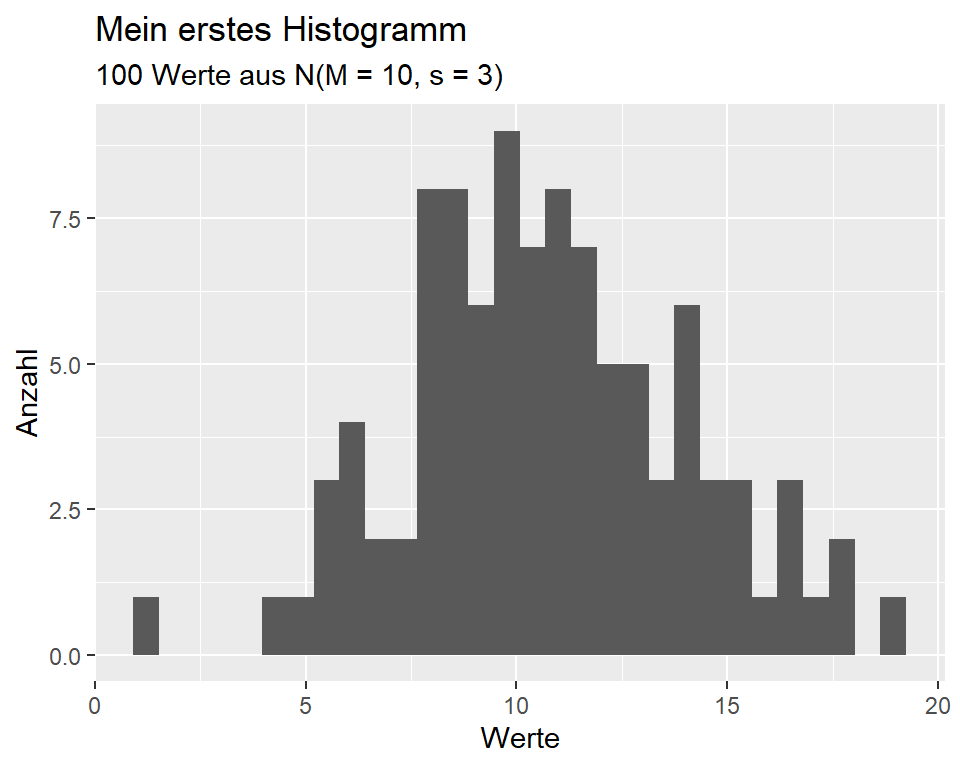
\includegraphics{statformulasbook_files/figure-latex/hist-fig-1} 

}

\caption{Ein Histogramm mit ggplot2}\label{fig:hist-fig}
\end{figure}

\begin{Shaded}
\begin{Highlighting}[]
\FunctionTok{library}\NormalTok{(kableExtra)}
\FunctionTok{options}\NormalTok{(}\AttributeTok{knitr.table.format =} \StringTok{"latex"}\NormalTok{)}
\end{Highlighting}
\end{Shaded}

\begin{Shaded}
\begin{Highlighting}[]
\CommentTok{\# Klassenbreite auf 2 anpassen und Balken mit weissen Linien trennen}
\FunctionTok{ggplot}\NormalTok{(}\AttributeTok{data =}\NormalTok{ daten, }\FunctionTok{aes}\NormalTok{(}\AttributeTok{x =}\NormalTok{ Werte)) }\SpecialCharTok{+}
  \FunctionTok{geom\_histogram}\NormalTok{(}\AttributeTok{binwidth =} \DecValTok{2}\NormalTok{, }\AttributeTok{color =} \StringTok{"white"}\NormalTok{) }\SpecialCharTok{+}
  \FunctionTok{xlab}\NormalTok{(}\StringTok{"Werte"}\NormalTok{) }\SpecialCharTok{+}
  \FunctionTok{ylab}\NormalTok{(}\StringTok{"Anzahl"}\NormalTok{) }\SpecialCharTok{+}
  \FunctionTok{ggtitle}\NormalTok{(}\StringTok{"Mein zweites Histogramm"}\NormalTok{, }\AttributeTok{subtitle =} \StringTok{"100 Werte aus N(M = 10, s = 3)"}\NormalTok{)  }
\end{Highlighting}
\end{Shaded}

\begin{figure}

{\centering 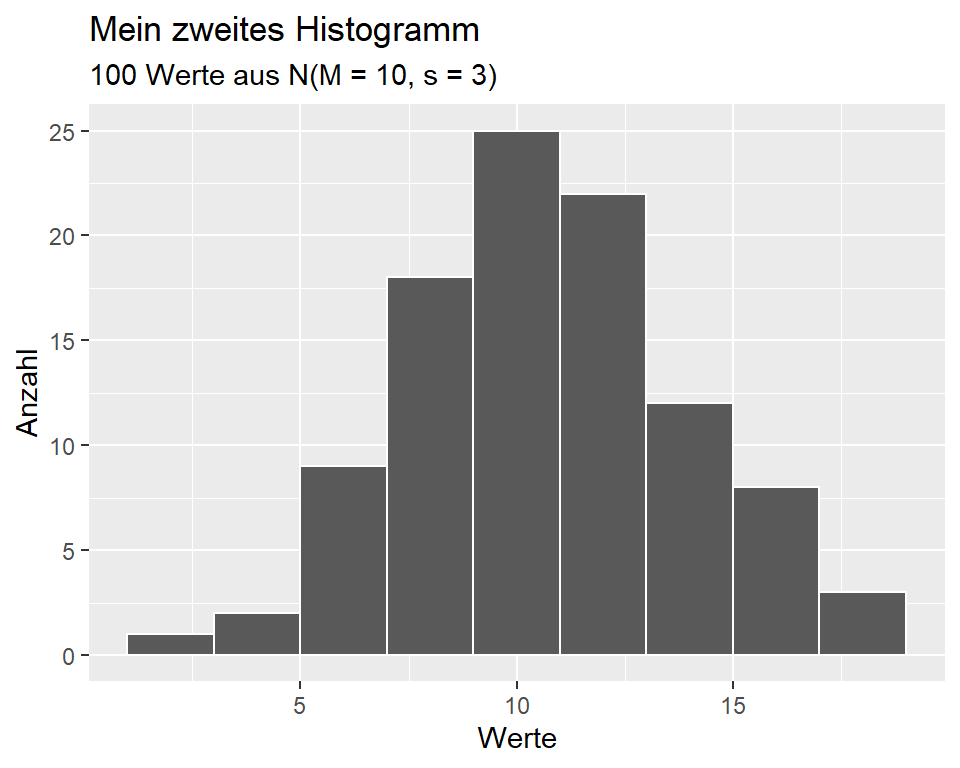
\includegraphics{statformulasbook_files/figure-latex/hist2-fig-1} 

}

\caption{Noch ein Histogramm mit ggplot2}\label{fig:hist2-fig}
\end{figure}

Für weitere Details siehe z.B. \href{https://www.r-graph-gallery.com/220-basic-ggplot2-histogram.html}{The R Graph Gallery}

\hypertarget{boxplot}{%
\subsection{Boxplot}\label{boxplot}}

Voraussetzung: Daten sind quantitativ

\begin{Shaded}
\begin{Highlighting}[]
\CommentTok{\# Beispieldatensatz mit Zufallszahlen aus Normalverteilung erzeugen}
\FunctionTok{set.seed}\NormalTok{(}\DecValTok{1234}\NormalTok{)}
\NormalTok{daten }\OtherTok{\textless{}{-}} \FunctionTok{data.frame}\NormalTok{(}
\NormalTok{  Werte }\OtherTok{\textless{}{-}} \FunctionTok{rnorm}\NormalTok{(}\DecValTok{100}\NormalTok{, }\AttributeTok{mean =} \DecValTok{10}\NormalTok{, }\AttributeTok{sd =} \DecValTok{3}\NormalTok{) }
\NormalTok{)}

\FunctionTok{ggplot}\NormalTok{(}\AttributeTok{data =}\NormalTok{ daten, }\FunctionTok{aes}\NormalTok{(}\AttributeTok{y =}\NormalTok{ Werte)) }\SpecialCharTok{+}
  \FunctionTok{geom\_boxplot}\NormalTok{() }\SpecialCharTok{+}
  \FunctionTok{ggtitle}\NormalTok{(}\StringTok{"Mein erster Boxplot"}\NormalTok{, }\AttributeTok{subtitle =} \StringTok{"100 Werte aus N(M = 10, s = 3)"}\NormalTok{)}
\end{Highlighting}
\end{Shaded}

\begin{figure}

{\centering 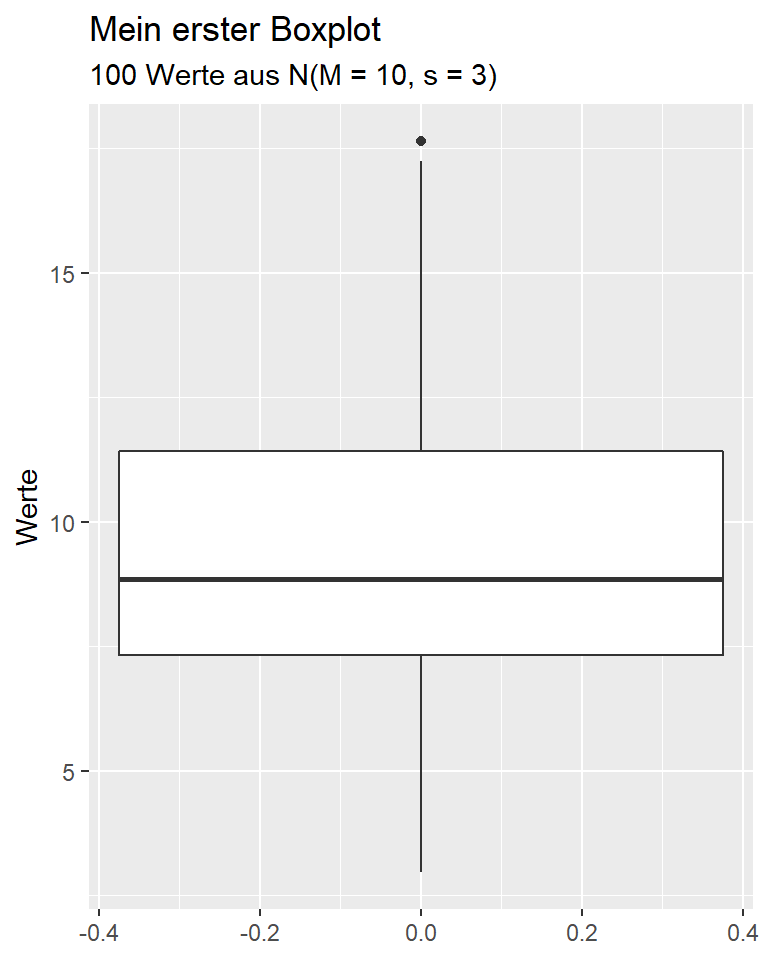
\includegraphics{statformulasbook_files/figure-latex/boxplot-fig-1} 

}

\caption{Ein Boxplot mit ggplot2}\label{fig:boxplot-fig}
\end{figure}

Boxplots eignen sich gut für den Vergleich von Gruppen.

\begin{Shaded}
\begin{Highlighting}[]
\CommentTok{\# Beispieldatensatz für Körpergrösse von Frauen und Männerenerzeugen}
\FunctionTok{set.seed}\NormalTok{(}\DecValTok{1234}\NormalTok{)}
\NormalTok{daten }\OtherTok{\textless{}{-}} \FunctionTok{data.frame}\NormalTok{(}
\NormalTok{  Geschlecht }\OtherTok{\textless{}{-}} \FunctionTok{c}\NormalTok{(}\FunctionTok{rep}\NormalTok{(}\StringTok{"w"}\NormalTok{, }\DecValTok{50}\NormalTok{), }\FunctionTok{rep}\NormalTok{(}\StringTok{"m"}\NormalTok{, }\DecValTok{50}\NormalTok{)),}
\NormalTok{  Groesse }\OtherTok{\textless{}{-}} \FunctionTok{c}\NormalTok{(}\FunctionTok{rnorm}\NormalTok{(}\DecValTok{50}\NormalTok{, }\AttributeTok{mean =} \DecValTok{165}\NormalTok{, }\AttributeTok{sd =} \DecValTok{6}\NormalTok{), }\FunctionTok{rnorm}\NormalTok{(}\DecValTok{50}\NormalTok{, }\DecValTok{178}\NormalTok{, }\DecValTok{7}\NormalTok{))}
\NormalTok{)}

\FunctionTok{ggplot}\NormalTok{(}\AttributeTok{data =}\NormalTok{ daten, }\FunctionTok{aes}\NormalTok{(}\AttributeTok{y =}\NormalTok{ Groesse, }\AttributeTok{x =}\NormalTok{ Geschlecht)) }\SpecialCharTok{+}
  \FunctionTok{geom\_boxplot}\NormalTok{() }\SpecialCharTok{+}
  \FunctionTok{ylab}\NormalTok{(}\StringTok{"Groesse in cm"}\NormalTok{) }\SpecialCharTok{+}
  \FunctionTok{ggtitle}\NormalTok{(}\StringTok{"Körpergrösse von Frauen und Männern"}\NormalTok{, }\AttributeTok{subtitle =} \StringTok{"n = 50 pro Geschlecht"}\NormalTok{)}
\end{Highlighting}
\end{Shaded}

\begin{figure}

{\centering 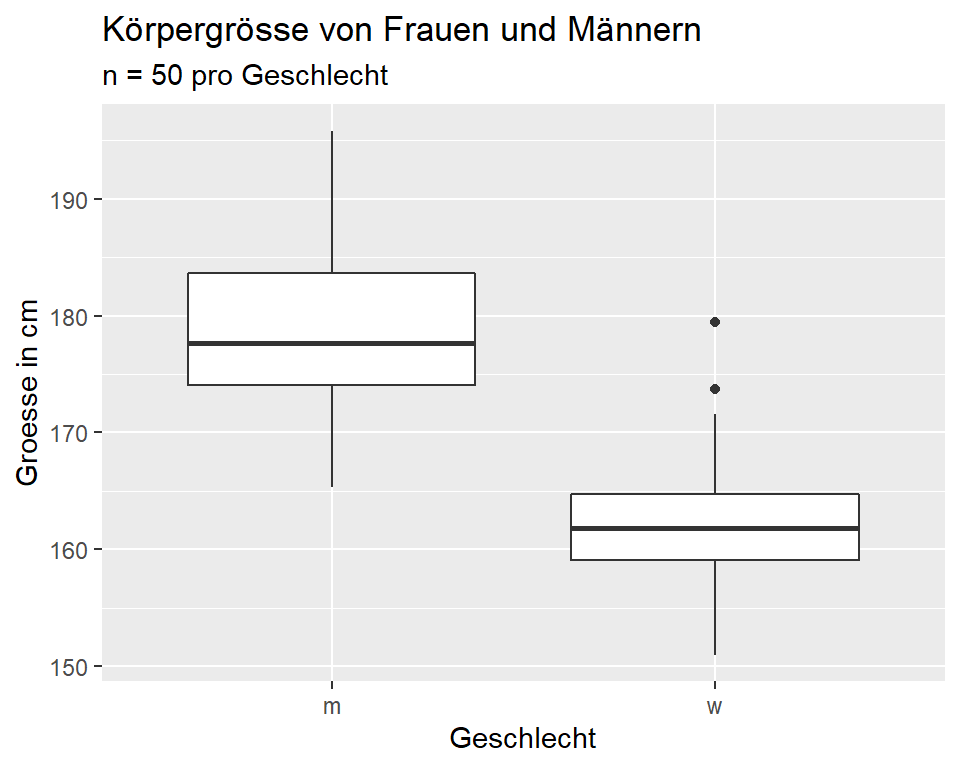
\includegraphics{statformulasbook_files/figure-latex/boxplot2-fig-1} 

}

\caption{Gruppierter Boxplot mit ggplot2}\label{fig:boxplot2-fig}
\end{figure}

Für weitere Details siehe z.B. \href{https://www.r-graph-gallery.com/262-basic-boxplot-with-ggplot2.html}{The R Graph Gallery}

\hypertarget{balkendiagramm}{%
\subsection{Balkendiagramm}\label{balkendiagramm}}

Voraussetzung: Daten sind qualitativ

\begin{Shaded}
\begin{Highlighting}[]
\CommentTok{\# Beispieldatensatz für Augenfarben von 50 Personen  }
\NormalTok{daten }\OtherTok{\textless{}{-}} \FunctionTok{data.frame}\NormalTok{(}
\NormalTok{  Augenfarbe }\OtherTok{\textless{}{-}} \FunctionTok{c}\NormalTok{(}\FunctionTok{rep}\NormalTok{(}\StringTok{"blau"}\NormalTok{, }\DecValTok{20}\NormalTok{), }\FunctionTok{rep}\NormalTok{(}\StringTok{"braun"}\NormalTok{, }\DecValTok{18}\NormalTok{), }\FunctionTok{rep}\NormalTok{(}\StringTok{"grün"}\NormalTok{, }\DecValTok{12}\NormalTok{))}
\NormalTok{)}

\FunctionTok{ggplot}\NormalTok{(}\AttributeTok{data =}\NormalTok{ daten, }\FunctionTok{aes}\NormalTok{(}\AttributeTok{x =}\NormalTok{ Augenfarbe)) }\SpecialCharTok{+}
  \FunctionTok{geom\_bar}\NormalTok{() }\SpecialCharTok{+}
  \FunctionTok{ylab}\NormalTok{(}\StringTok{"Anzahl"}\NormalTok{) }\SpecialCharTok{+}
  \FunctionTok{ggtitle}\NormalTok{(}\StringTok{"Augenfarben, n = 50"}\NormalTok{)}
\end{Highlighting}
\end{Shaded}

\begin{figure}

{\centering 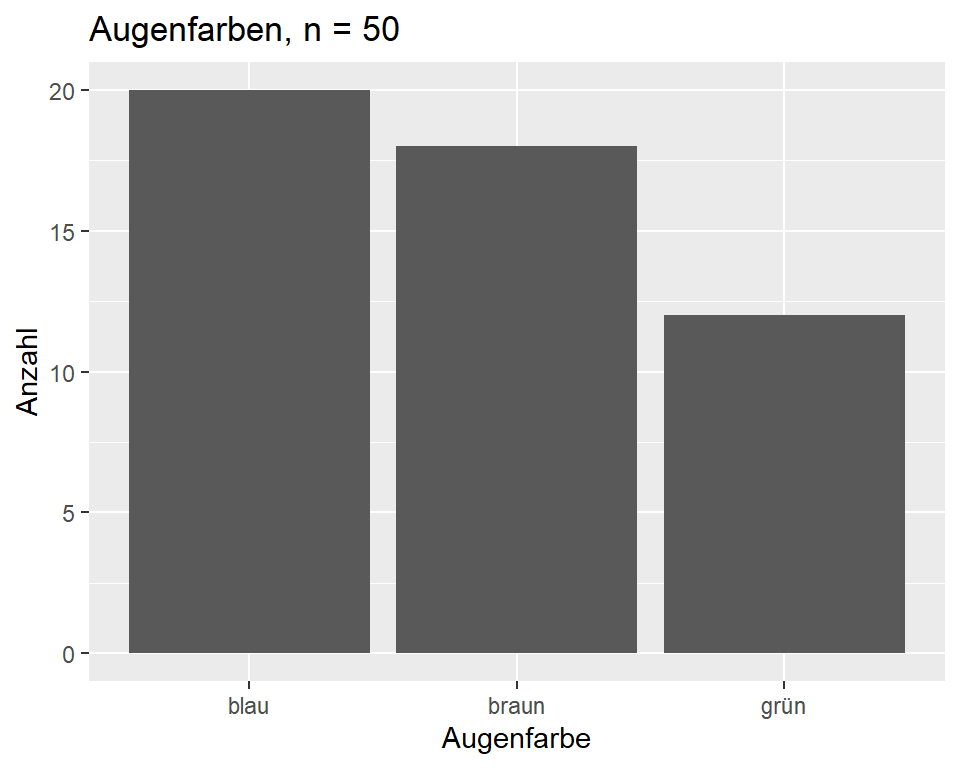
\includegraphics{statformulasbook_files/figure-latex/barplot-fig-1} 

}

\caption{Balkendiagramm mit ggplot2}\label{fig:barplot-fig}
\end{figure}

Balken können z.B. eingefärbt werden (\texttt{R} verfügt über 657 Farben, siehe z.B. \href{http://sape.inf.usi.ch/quick-reference/ggplot2/colour}{hier} )

\begin{Shaded}
\begin{Highlighting}[]
\FunctionTok{ggplot}\NormalTok{(}\AttributeTok{data =}\NormalTok{ daten, }\FunctionTok{aes}\NormalTok{(}\AttributeTok{x =}\NormalTok{ Augenfarbe)) }\SpecialCharTok{+}
  \FunctionTok{geom\_bar}\NormalTok{(}\AttributeTok{fill =} \FunctionTok{c}\NormalTok{(}\StringTok{"blue"}\NormalTok{, }\StringTok{"brown"}\NormalTok{, }\StringTok{"green"}\NormalTok{)) }\SpecialCharTok{+}
  \FunctionTok{ylab}\NormalTok{(}\StringTok{"Anzahl"}\NormalTok{) }\SpecialCharTok{+}
  \FunctionTok{ggtitle}\NormalTok{(}\StringTok{"Augenfarben, n = 50"}\NormalTok{)}
\end{Highlighting}
\end{Shaded}

\begin{figure}

{\centering 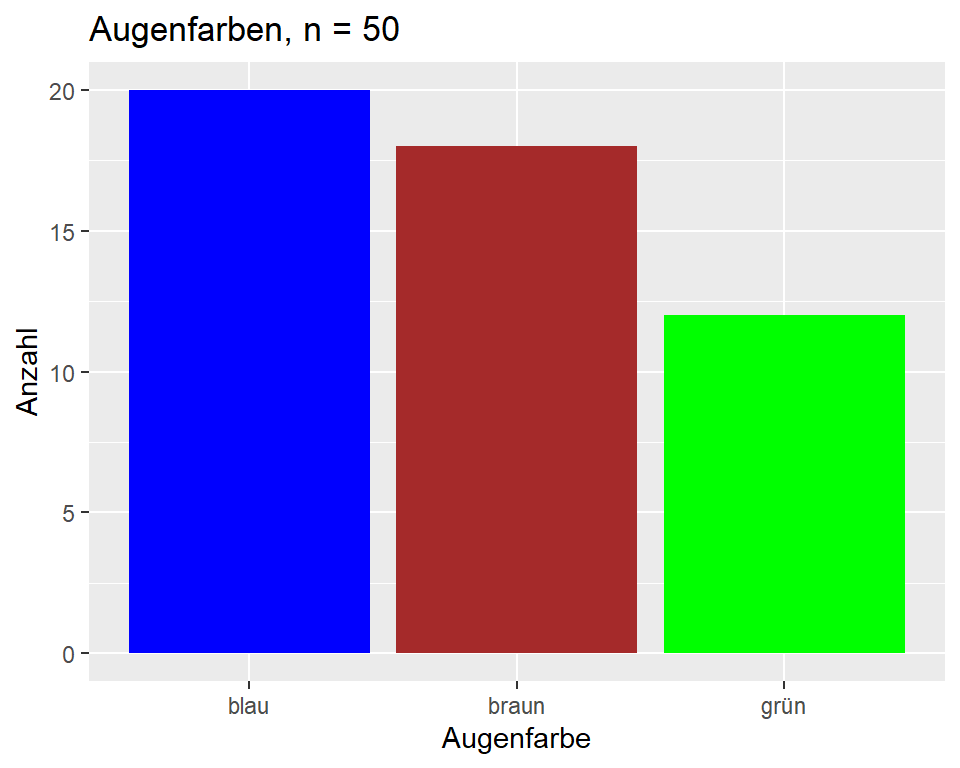
\includegraphics{statformulasbook_files/figure-latex/barplot2-fig-1} 

}

\caption{Hübsches Balkendiagramm mit ggplot2}\label{fig:barplot2-fig}
\end{figure}

Für weitere Details siehe z.B. \href{https://www.r-graph-gallery.com/barplot.html}{The R Graph Gallery}

\hypertarget{tabellen-fuxfcr-huxe4ufigkeiten}{%
\subsection{Tabellen für Häufigkeiten}\label{tabellen-fuxfcr-huxe4ufigkeiten}}

Tabelle mit absoluten Häufigkeiten für die Augenfarben erstellen.

\begin{Shaded}
\begin{Highlighting}[]
\FunctionTok{table}\NormalTok{(daten}\SpecialCharTok{$}\NormalTok{Augenfarbe)}
\end{Highlighting}
\end{Shaded}

\begin{verbatim}
## 
##  blau braun  grün 
##    20    18    12
\end{verbatim}

Tabelle mit den relativen Häufigkeiten für die Augenfarben erstellen.

\begin{Shaded}
\begin{Highlighting}[]
\FunctionTok{prop.table}\NormalTok{(}\FunctionTok{table}\NormalTok{(daten}\SpecialCharTok{$}\NormalTok{Augenfarbe))}
\end{Highlighting}
\end{Shaded}

\begin{verbatim}
## 
##  blau braun  grün 
##  0.40  0.36  0.24
\end{verbatim}

\hypertarget{grundbegriffe-der-wahrscheinlichkeitstheorie}{%
\chapter{Grundbegriffe der Wahrscheinlichkeitstheorie}\label{grundbegriffe-der-wahrscheinlichkeitstheorie}}

\hypertarget{wahrscheinlichkeit}{%
\section{Wahrscheinlichkeit}\label{wahrscheinlichkeit}}

\begin{itemize}
\tightlist
\item
  Unter Wahrscheinlichkeit versteht man die Chance, dass bei einem Zufallsexperiment ein bestimmtes Ereignis auftritt.\\
\item
  Wahrscheinlichkeiten können nur Werte zwischen 0 (unmögliches Ereignis) und 1 (sicheres Ereignis) zugeordnet werden.\\
\item
  Nach \emph{Laplace} ist die Wahrscheinlichkeit für ein günstiges Ereignis \(p(A)\):
\end{itemize}

\begin{equation}
  p(A) = \frac{n_A}{N_{gesamt}} = \frac{Anzahl~der~günstigen~Ereignisse}{Anzahl~der~möglichen~Ereignisse}
  \label{eq:prob-p}
\end{equation}

\hypertarget{ereignis-und-komplementuxe4rereignis}{%
\section{Ereignis und Komplementärereignis}\label{ereignis-und-komplementuxe4rereignis}}

\begin{equation}
  p(A) + p(Nicht~A) = 1
  \label{eq:prob-p-q}
\end{equation}

\hypertarget{disjunkte-ereignisse}{%
\section{Disjunkte Ereignisse}\label{disjunkte-ereignisse}}

Zwei Ereignisse A und B werden als \emph{disjunkt} bezeichnet, wenn sie einander ausschliessen, d.h. dass A und B nicht gleichzeitig eintreffen können.

\begin{equation}
  A \cap B = 0
  \label{eq:disjoint}
\end{equation}

Lese die Formel: Zwei Ereignisse A und B sind disjunkt, wenn die Schnittmenge der leeren Menge entspricht.

\hypertarget{nicht-disjunkte-ereignisse}{%
\section{Nicht-disjunkte Ereignisse}\label{nicht-disjunkte-ereignisse}}

Zwei Ereignisse A und B werden als \emph{nicht-disjunkt} bezeichnet, wenn die Wahrscheinlichkeit für das gleichzeitige Auftreten deser Ereignisse nicht gleich null ist.

\begin{equation}
  A \cap B \neq 0
  \label{eq:disjoint}
\end{equation}

Lese die Formel: Nicht-disjunkte Ereignisse haben eine nicht leere Schnittmenge.

\hypertarget{bedingte-wahrscheinlichkeiten}{%
\section{Bedingte Wahrscheinlichkeiten}\label{bedingte-wahrscheinlichkeiten}}

Die bedingte Wahrscheinlichkeit \(p(A|B)\) quantifiziert die Wahrscheinlichkeit des Ereignisses A unter der Bedingung, dass das Ereignis B eingetreten ist.

\begin{equation}
  p(A|B) = \frac{p(A \cap B)}{P(B)}
  \label{eq:condprob}
\end{equation}

Das Zeichen \(\cap\) ist das mathematische Symbol für UND (Schnittmenge von A und B).

\hypertarget{unabhuxe4ngigkeit}{%
\section{Unabhängigkeit}\label{unabhuxe4ngigkeit}}

Zwei Ereignisse \(A\) und \(B\) sind unabhängig, wenn das Eintreffen oder Nicht-Eintreffen des Ereignisses \(B\) die Wahrscheinlichkeit für ein Ereignis \(A\) nicht verändert.

\begin{equation}
  p(A) = p(A|B) ~, ~p(B) = p(B|A)
  \label{eq:independency}
\end{equation}

\hypertarget{theorem-von-bayes}{%
\section{Theorem von Bayes}\label{theorem-von-bayes}}

Das \emph{Theorem von Bayes} gibt an, wie man eine bedingte Wahrscheinlichkeit \(p(A|B)\) aus der umgekehrten bedingten Wahrscheinlichkeit \(p(B|A)\) berechnen kann.

\begin{equation}
  p(A|B)= \frac{p(A) \times p(B|A)}{p(B)}
  \label{eq:bayes}
\end{equation}

\hypertarget{wahrscheinlichkeitsverteilungen}{%
\chapter{Wahrscheinlichkeitsverteilungen}\label{wahrscheinlichkeitsverteilungen}}

\textbf{Diskrete Wahrscheinlichkeitsverteilung}

Die Ergebnisse eines Zufallsexperiments mit einer diskreten Variablen sind abzählbar
bzw. können kategorisiert werden. Beispielsweise ist es beim Werfen eines Würfels
nur möglich eine Zahl aus der Menge \(X = {1, 2, 3, 4, 5, 6}\) zu werfen. Der Wurf einer
2.6 ist jedoch nicht möglich. Die Anzahl der Seiten eines Würfels könnten gezählt und kategorisiert werden. Daher handelt es sich hierbei um eine diskrete Verteilung \citep{Leonhart2013}.

\textbf{Kontinuierliche (= stetige) Wahrscheinlichkeitsverteilung}

Stetige Wahrscheinlichkeitsfunktionen beschreiben die Ergebnisse eines Zufallsexperiments, in dem unendlich viele Elementarereignisse realisiert werden können. So entsteht eine stetige \emph{Dichtefunktion} der Wahrscheinlichkeitsverteilung \citep{Leonhart2013}.

Die Betrachtung eines einzelnen Ereignisses in einer stetigen Wahrscheinlichkeitsverteilung ist nicht sinnvoll, da die Wahrscheinlichkeit für ein Elementarereignis immer gegen null geht. Es ist sehr unwahrscheinlich, dass eine Studentin mit genau 167.793 cm Grösse an einer Lehrveranstaltung teilnimmt.

Deshalb wir die Wahrscheinlichkeit für Intervalle zwischen zwei Elementarereignissen bestimmt. Diese Wahrscheinlichkeit entspricht der Fläche (dem Integral) der Dichtefunktion der stetigen Wahrscheinlichkeitsverteilung in diesen Grenzen \citep{Leonhart2013}.

\hypertarget{binomialverteilung}{%
\section{Binomialverteilung}\label{binomialverteilung}}

Die Binomialverteilung beschreibt die Auftretenswahrscheinlichkeit zweier alternativer Ereignisse. Sie wird durch einen \emph{Bernoulli-Prozess} erzeugt. Dies ist eine Folge voneinander unabhängiger Ereignisse mit jeweils zwei möglichen Ausgängen. Die Wahrscheinlichkeiten für die einzelnen Ereignisse sind jeweils konstant (\(p\) bzw. \(q = 1 - p\)) \citep{Leonhart2013}.

\hypertarget{voraussetzungen}{%
\subsection{Voraussetzungen}\label{voraussetzungen}}

\begin{itemize}
\tightlist
\item
  Die Versuche müssen unabhängig sein.\\
\item
  Die Anzahl der Versuche muss bekannt sein.\\
\item
  Jedes Versuchsergebnis ist entweder ein Erfolg oder ein Misserfolg.\\
\item
  Die Wahrscheinlichkeit für einen Erfolg muss für jeden Versuch gleich sein.
\end{itemize}

\hypertarget{funktion-der-binomialverteilung}{%
\subsection{Funktion der Binomialverteilung}\label{funktion-der-binomialverteilung}}

Die Funktion der Binomialverteilung beschreibt die Wahrscheinlichkeit des \(k\)-maligen Eintreffens eines Ereignisses X bei \(n\) Ereignissen

Wenn \(p\) die Wahrscheinlichkeit für einen Erfolg ist, ist \(1-p\) die Wahrscheinlichkeit für einen Misserfolg. \(n\) gibt die Anzahl der Versuche an und \(k\) die Anzahl der Erfolge.

\begin{equation}
  p(k, n) =  {n \choose k}p^k(1-p)^{n-k}
  \label{eq:binom}
\end{equation}

Die Gleichung setzt sich aus drei Faktoren zusammen:

\begin{itemize}
\tightlist
\item
  \(n \choose k\) (sprich n über k) gibt die Anzahl aller möglichen Reihenfolgen an,
  die zu dem erwünschten Ereignis führen. Dieser Faktor wird als \emph{Binomialkoeffizient} bezeichnet.\\
\item
  \(p^k\) ist die Wahrscheinlichkeit für das k-malige Eintreten eines Erfolgs.\\
\item
  \((1-p)^{n-k}\) ist die Wahrscheinlichkeit für das \((n-k)\)-malige Eintreffen des Komplementärereignisses.
\end{itemize}

Wahrscheinlichkeit für \(k\) Erfolge in \(n\) Versuchen mit der Erfolgswahrscheinlichkeit \(p\) in \texttt{R} berechnen:

\begin{Shaded}
\begin{Highlighting}[]
\CommentTok{\# R: Dichtefunktion der Binomialverteilung}
\FunctionTok{dbinom}\NormalTok{(k, n, p)}
\end{Highlighting}
\end{Shaded}

Beispiel: Wie gross ist die Wahrscheinlichkeit, bei drei Mal würfeln (\(n\) = 3), 1 bis 3 mal (\(k\) = 0 bis 3) eine bestimmte Zahl, z.B. eine 6 (\(p\) = 1/6) zu werfen?

\begin{Shaded}
\begin{Highlighting}[]
\NormalTok{p }\OtherTok{\textless{}{-}} \DecValTok{1}\SpecialCharTok{/}\DecValTok{6}
\NormalTok{n }\OtherTok{\textless{}{-}} \DecValTok{3}
\NormalTok{k }\OtherTok{\textless{}{-}} \DecValTok{1}\SpecialCharTok{:}\DecValTok{3}

\FunctionTok{dbinom}\NormalTok{(k, }\AttributeTok{size =}\NormalTok{ n, }\AttributeTok{prob =}\NormalTok{ p)}
\end{Highlighting}
\end{Shaded}

\begin{verbatim}
## [1] 0.34722222 0.06944444 0.00462963
\end{verbatim}

\hypertarget{binomialkoeffizient}{%
\subsection{Binomialkoeffizient}\label{binomialkoeffizient}}

Der Binomialkoeffizient gibt an, auf wie viele verschiedene Arten man \(k\) Objekte aus einer Menge von \(n\) verschiedenen Objekten auswählen kann.

Anzahl Kombinationen von \(k\) Erfolgen in \(n\) Versuchen berechnen

\begin{equation}
 {n \choose k} = \frac{n!}{k!(n-k)!}
 \label{eq:binomkoef}
\end{equation}

\begin{Shaded}
\begin{Highlighting}[]
\CommentTok{\# R: Binomialkoeffizient}
\FunctionTok{choose}\NormalTok{(n, k)}
\end{Highlighting}
\end{Shaded}

Beispiel: Wieviele mögliche Kombinationen gibt es im Schweizer Zahlenlotto für 6 (= \(k\)) aus 42 (=\(n\)).

\begin{Shaded}
\begin{Highlighting}[]
\FunctionTok{choose}\NormalTok{(}\AttributeTok{n =} \DecValTok{42}\NormalTok{, }\AttributeTok{k =} \DecValTok{6}\NormalTok{)}
\end{Highlighting}
\end{Shaded}

\begin{verbatim}
## [1] 5245786
\end{verbatim}

Es gibt \(\ensuremath{5.245786\times 10^{6}}\) Kombinationen, d.h. die Wahrscheinlichkeit, 6 Richtige zu wählen beträgt 1\(/\ensuremath{5.245786\times 10^{6}}\) = \(\ensuremath{1.906292\times 10^{-7}}\).

\hypertarget{eigenschaften-der-binomialverteilung}{%
\subsection{Eigenschaften der Binomialverteilung}\label{eigenschaften-der-binomialverteilung}}

\begin{equation}
  X \sim Bin(n, p)
  \label{eq:binom2}
\end{equation}

\(n\) = Anzahl Versuche\\
\(p\) = Eintrittswahrscheinlichkeit

\textbf{Erwartungswert (Mittelwert) der Binomialverteilung}

\begin{equation}
  \mu = n \times p
  \label{eq:mubinom}
\end{equation}

\textbf{Standardabweichung der Binomialverteilung}

\begin{equation}
  \sigma = \sqrt{np(1-p)}
  \label{eq:sigmabinom}
\end{equation}

\hypertarget{normalapproximation}{%
\subsection{Normalapproximation}\label{normalapproximation}}

Eine Binomialverteilung mit mindestens 10 erwarteten Erfolgen und mindestens 10 erwarteten Misserfolgen folgt annähernd einer Normalverteilung.

\[n \times p \times (1-p) \geq 10\]

Falls diese Bedingung erfüllt ist, gilt:

\begin{equation}
  Bin(n, p) \sim N(\mu, \sigma)
  \label{eq:binomnormapprox}
\end{equation}

\hypertarget{normalverteilung}{%
\section{Normalverteilung}\label{normalverteilung}}

\begin{equation}
  X \sim N(\mu, \sigma)
  \label{eq:normdistr}
\end{equation}

\hypertarget{regel}{%
\subsection{68-95-99.7-Regel}\label{regel}}

\begin{itemize}
\tightlist
\item
  68\% in \(\mu \pm 1\sigma\)\\
\item
  95\% in \(\mu \pm 2\sigma\), genauer \(\mu \pm 1.96\sigma\)\\
\item
  99.7\% in \(\mu \pm 3\sigma\)
\end{itemize}

\hypertarget{standardnormalverteilung}{%
\subsection{Standardnormalverteilung}\label{standardnormalverteilung}}

\begin{equation}
  X \sim N(0, 1)
  \label{eq:stdnormdistr}
\end{equation}

\hypertarget{z-wert}{%
\subsection{z-Wert}\label{z-wert}}

Der z-Wert einer Beobachtung \(x_i\) gibt an, um wieviele Standardabweichungen die Beobachtung über oder unter dem Mittelwert liegt.

\begin{equation}
  z = \frac{x_i-\bar{x}}{s}
  \label{eq:zvalue}
\end{equation}

Der z-Wert des Mittelwerts ist 0.\\
Ungewöhnliche Beobachtungen haben typischerweise einen z-Wert von \(|z|>2\).

\hypertarget{wahrscheinlichkeiten-und-perzentilen-in-r-berechnen}{%
\subsection{\texorpdfstring{Wahrscheinlichkeiten und Perzentilen in \texttt{R} berechnen}{Wahrscheinlichkeiten und Perzentilen in R berechnen}}\label{wahrscheinlichkeiten-und-perzentilen-in-r-berechnen}}

\begin{Shaded}
\begin{Highlighting}[]
\FunctionTok{pnorm}\NormalTok{(x, mean, sd)                      }\CommentTok{\# Fläche links von x }

\DecValTok{1} \SpecialCharTok{{-}} \FunctionTok{pnorm}\NormalTok{(x, mean, sd)                  }\CommentTok{\# Fläche rechts von x}
\FunctionTok{pnorm}\NormalTok{(x, mean, sd, }\AttributeTok{lower.tail =} \ConstantTok{FALSE}\NormalTok{)  }\CommentTok{\# Fläche rechts von x (alternativ)}

\FunctionTok{qnorm}\NormalTok{(percentile, mean, sd)             }\CommentTok{\# \# Wert auf einer bestimmten Perzentile}
\end{Highlighting}
\end{Shaded}

Beispiel:

\begin{Shaded}
\begin{Highlighting}[]
\NormalTok{x }\OtherTok{\textless{}{-}} \FunctionTok{c}\NormalTok{(}\DecValTok{2}\NormalTok{, }\DecValTok{3}\NormalTok{, }\DecValTok{4}\NormalTok{, }\DecValTok{4}\NormalTok{, }\DecValTok{5}\NormalTok{, }\DecValTok{6}\NormalTok{, }\DecValTok{10}\NormalTok{, }\DecValTok{9}\NormalTok{, }\DecValTok{8}\NormalTok{, }\DecValTok{7}\NormalTok{, }\DecValTok{7}\NormalTok{, }\DecValTok{7}\NormalTok{, }\DecValTok{5}\NormalTok{, }\DecValTok{4}\NormalTok{)}
\NormalTok{mittelwert }\OtherTok{\textless{}{-}} \FunctionTok{mean}\NormalTok{(x)}
\NormalTok{stdabw }\OtherTok{\textless{}{-}} \FunctionTok{sd}\NormalTok{(x)}

\CommentTok{\# Wahrscheinlichkeit für den Wert kleiner oder gleich 7}
\FunctionTok{pnorm}\NormalTok{(}\DecValTok{7}\NormalTok{, mittelwert, stdabw)}
\end{Highlighting}
\end{Shaded}

\begin{verbatim}
## [1] 0.6991514
\end{verbatim}

\begin{Shaded}
\begin{Highlighting}[]
\CommentTok{\# Wahrscheinlichkeit für den Wert gleich oder grösser 7}
\DecValTok{1} \SpecialCharTok{{-}} \FunctionTok{pnorm}\NormalTok{(}\DecValTok{7}\NormalTok{, mittelwert, stdabw)}
\end{Highlighting}
\end{Shaded}

\begin{verbatim}
## [1] 0.3008486
\end{verbatim}

\begin{Shaded}
\begin{Highlighting}[]
\CommentTok{\# Wert auf der 40\%{-}Perzentile}
\FunctionTok{qnorm}\NormalTok{(.}\DecValTok{4}\NormalTok{, mittelwert, stdabw)}
\end{Highlighting}
\end{Shaded}

\begin{verbatim}
## [1] 5.19633
\end{verbatim}

\hypertarget{qq-plot}{%
\subsection{QQ-Plot}\label{qq-plot}}

Mittels QQ-Plots (Quantile-Quantile-Plots) können zwei Verteilungen grafisch verglichen werden, indem ihre Quantilen gegeneinander aufgetragen werden. Wenn die zwei Verteilungen exakt gleich sind, liegen die Punkte im QQ-Plot auf einer perfekten Linie.

\begin{Shaded}
\begin{Highlighting}[]
\FunctionTok{qqnorm}\NormalTok{()    }\CommentTok{\# QQ{-}Plot für Normalverteilung}
\FunctionTok{qqline}\NormalTok{()    }\CommentTok{\# Linie in QQ{-}Plot einzeichnen}
\end{Highlighting}
\end{Shaded}

Beispiel:

\begin{Shaded}
\begin{Highlighting}[]
\FunctionTok{set.seed}\NormalTok{(}\DecValTok{1}\NormalTok{)}
\NormalTok{x }\OtherTok{\textless{}{-}} \FunctionTok{rnorm}\NormalTok{(}\DecValTok{100}\NormalTok{)         }\CommentTok{\# simulation von 100 normalverteilten Werten, mean = 0, s = 1}

\FunctionTok{qqnorm}\NormalTok{(x)               }\CommentTok{\# qq{-}plot erstellen}
\FunctionTok{qqline}\NormalTok{(x, }\AttributeTok{col =} \StringTok{"blue"}\NormalTok{) }\CommentTok{\# Linie in qq{-}plot einzeichnen}
\end{Highlighting}
\end{Shaded}

\begin{center}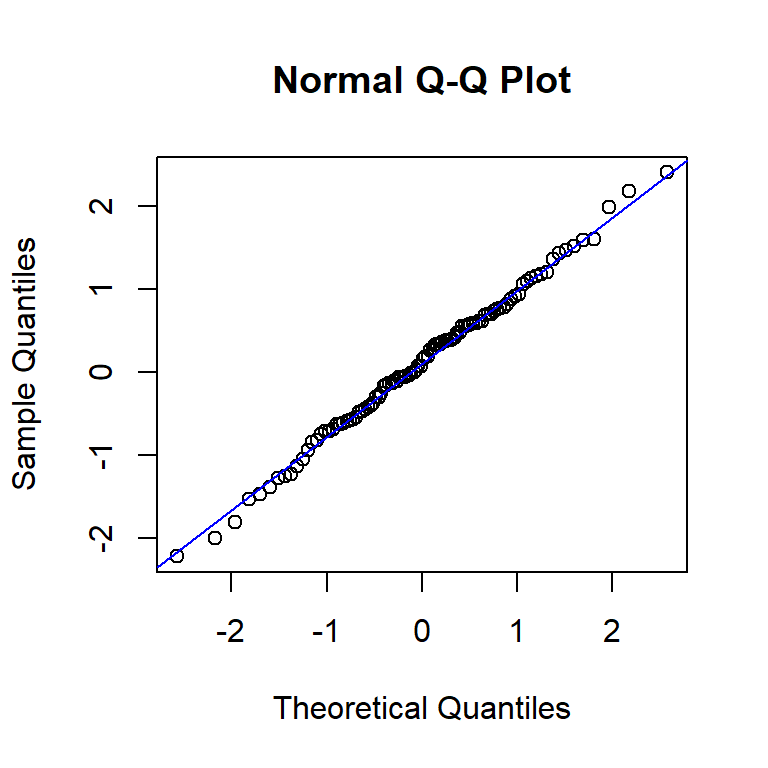
\includegraphics{statformulasbook_files/figure-latex/qq-fig-1} \end{center}

\begin{center}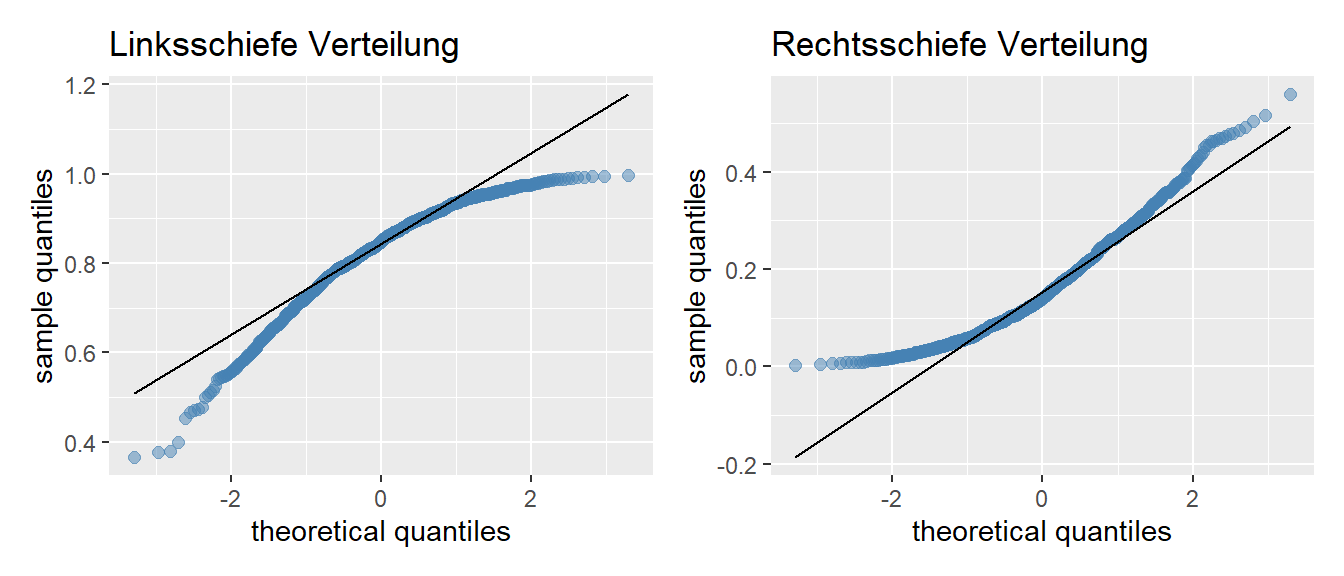
\includegraphics{statformulasbook_files/figure-latex/qq-fig2-1} \end{center}

\hypertarget{t-verteilung}{%
\section{\texorpdfstring{\(T\)-Verteilung}{T-Verteilung}}\label{t-verteilung}}

Die \(T\)-Verteilung

\begin{itemize}
\tightlist
\item
  kann als Variante der Normalverteilung aufgefasst werden.\\
\item
  hat immer den Mittelwert 0.\\
\item
  hat eine Standardabweichung, die vom Stichprobenumfang \(n\) abhängig ist.\\
\item
  Wird nur durch einen einzigen Parameter, die Anzahl Freiheitsgrade \(df\) (engl. degrees of freedom), definiert.\\
\item
  wird mit wachsendem \(n\) schmaler und geht für \(n \rightarrow \infty\) in die Normalverteilung über.
\end{itemize}

\[df = n-1\]
\[t \sim T(df)\]

Die \(T\)-verteilung wird verwendet, wenn

\begin{itemize}
\tightlist
\item
  der Stichprobenumfang klein ist (\(n \leq 30\))\\
\item
  die Standardabweichung \(\sigma\) der Population unbekannt ist und mit Hilfe der Stichprobenstandardabweichung \(s\) geschätzt werden muss.
\item
  also eigentlich immer; die Software rechnet standardmässig mit der \(T\)-Verteilung.\\
\item
  Die Teststatistik von \(T\)-Tests sind \(t\)-Werte. \(t\)-Werte werden gleich interpretiert wie \(z\)-Werte.
\end{itemize}

\begin{center}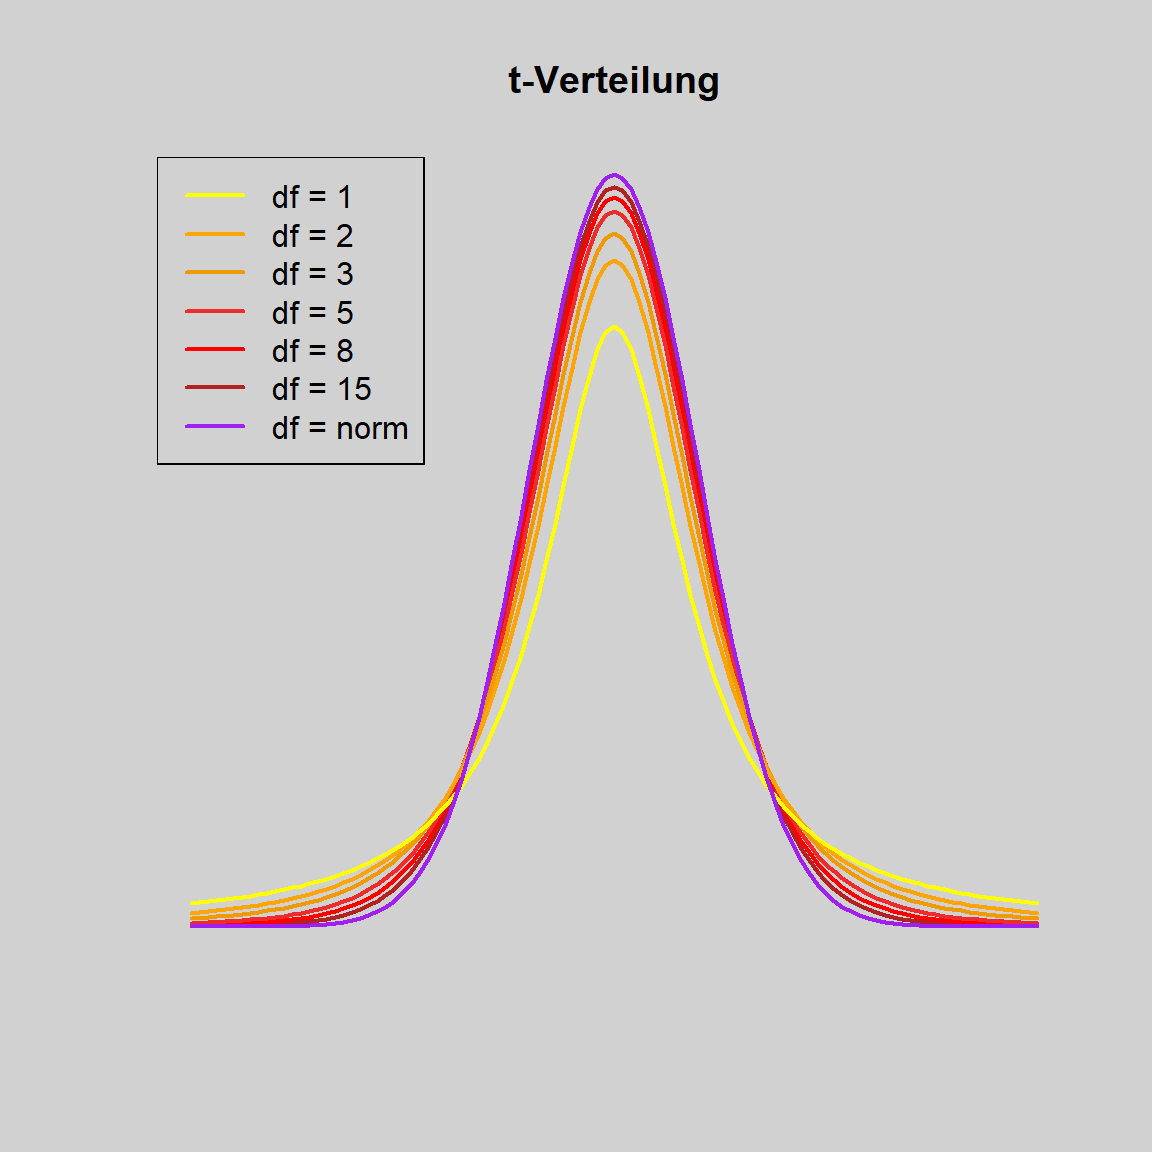
\includegraphics{statformulasbook_files/figure-latex/tdistr-fig-1} \end{center}

\hypertarget{grundlagen-der-inferenzstatistik}{%
\chapter{Grundlagen der Inferenzstatistik}\label{grundlagen-der-inferenzstatistik}}

\hypertarget{schuxe4tzungen-von-parametern}{%
\section{Schätzungen von Parametern}\label{schuxe4tzungen-von-parametern}}

Wird zur Schätzung eines Populationsparameters nur eine Stichprobenkennzahl angegeben, so handelt es sich um eine \emph{Punktschätzung}. Wird bei einer Schätzung neben der Kennzahl noch ein \emph{Konfidenzintervall} bestimmt, in welchem mit einer bestimmten Wahrscheinlichkeit der Populationsparameter liegt, so handelt es sich um eine \emph{Intervallschätzung}.

\hypertarget{schuxe4tzung-bei-qualitativen-merkmalen}{%
\subsection{Schätzung bei qualitativen Merkmalen}\label{schuxe4tzung-bei-qualitativen-merkmalen}}

\(p:\) Stichprobenkennzahl\\
\(\pi:\) Populationsparameter
Beide Kennzahlen können Werte zwischen 0 und 1 annehmen.

\textbf{95\%-Konfidenzintervall für \(\pi\)}

\begin{equation}
  CI_{95} = p \pm z_{0.975} \times s_p
  \label{eq:ciqualz}
\end{equation}

\begin{equation}
  s_p = \sqrt{\frac{p(1 - p)}{n}}
  \label{eq:sp}
\end{equation}

Bei Intervallschätzung mit kleinen Stichproben (N \textless{} 30, besser auch schon bei N \textless{} 100) sollte statt der Standardnormalverteilung (\(z\)-Werte) die Verteilung der \(t\)-Werte zur Definition des Intervalls zugrunde gelegt werden \citep{Leonhart2013}.

\begin{equation}
  CI_{95} = p \pm t_{0.975, df} \times s_p
  \label{eq:ciqualt}
\end{equation}

\hypertarget{schuxe4tzung-bei-quantitativen-merkmalen}{%
\subsection{Schätzung bei quantitativen Merkmalen}\label{schuxe4tzung-bei-quantitativen-merkmalen}}

\textbf{Zentraler Grenzwertsatz}

Die Verteilung von Stichprobenkennzahlen (z.B. Mittelwert) folgt annähernd einer Normalverteilung. Ihr Mittelwert liegt in der Nähe des Populationsmittelwertes \(\mu\) mit einer Standardabweichung geteilt durch die Quadratwurzel des Stichprobenumfangs (\emph{Standardfehler \(SE\)}).

\begin{equation}
  \bar{x} \sim N(Mittelwert = \mu, SE = \frac{\sigma}{\sqrt{n}})
  \label{eq:clt}
\end{equation}

Wenn \(\sigma\) unbekannt ist (was eigentlich immer der Fall ist), wird die Standardabweichung \(s\) der Stichprobe als Schätzer für \(\sigma\) eingesetzt.

\begin{equation}
  SE = \frac{s}{\sqrt{n}}
  \label{eq:se}
\end{equation}

Bedingungen für die Gültigkeit des zentralen Grenzwertsatzes:

Die Beobachtungseinheiten in der Stichprobe sind unabhängig voneinander (zufällige Auswahl, zufällige Zuordnung zu Gruppen).\\
Faustregel: Stichprobenumfang \(n>30\)

Beispiel für die Berechnung des Standardfehlers \(SE\) in \texttt{R}

\begin{Shaded}
\begin{Highlighting}[]
\FunctionTok{set.seed}\NormalTok{(}\DecValTok{1234}\NormalTok{)}
\NormalTok{x }\OtherTok{\textless{}{-}} \FunctionTok{rnorm}\NormalTok{(}\DecValTok{100}\NormalTok{)  }\CommentTok{\# simulation von 100 normalverteilten Werten, mean = 0, s = 1}

\NormalTok{n }\OtherTok{\textless{}{-}} \FunctionTok{length}\NormalTok{(x)   }\CommentTok{\# Stichprobenumfang von x ermitteln}
\NormalTok{s }\OtherTok{\textless{}{-}} \FunctionTok{sd}\NormalTok{(x)       }\CommentTok{\# Standardabweichung von x berechnen}

\NormalTok{s}\SpecialCharTok{/}\FunctionTok{sqrt}\NormalTok{(n)        }\CommentTok{\# Berechnung und Ausgabe von SE}
\end{Highlighting}
\end{Shaded}

\begin{verbatim}
## [1] 0.1004
\end{verbatim}

\textbf{95\%-Konfidenzintervall für \(\mu\)}

Konfidenzintervalle (Vertrauensintervalle, \(CI\)) können auf jedem Konfidenzniveau berechnet werden. Um die Sache nicht allzu kompliziert zu machen, wird hier v.a. exemplarisch die Berechnung von 95\%-Konfidenzinteravallen vorgestellt.

Signifikanzniveau = \(\alpha\)
Konfidenzniveau = \(1-\alpha\)

\begin{equation}
  CI_{95} = \bar{x} \pm z_{0.975} \times SE
  \label{eq:cinorm}
\end{equation}

Allgemein formuliert:

\begin{equation}
  CI^* = \bar{x} \pm z^* \times SE
  \label{eq:cinorm}
\end{equation}

\begin{equation}
  z^* = \vert \frac{(1-CI^*)}{2} \vert
  \label{eq:zforci}
\end{equation}

\begin{equation}
  z^* \times SE = z^* \times \frac{s}{\sqrt{n}}
  \label{eq:ME}
\end{equation}

\(z^* \times SE\) wird auch als Fehlerbereich (engl. \(margin~ of~ error,~ ME\)) bezeichnet.
Der Wert von \(z^*\) ist abhängig vom Konfidenzniveau.

\begin{Shaded}
\begin{Highlighting}[]
\CommentTok{\# z für ein 95\% CI}
\NormalTok{CI }\OtherTok{\textless{}{-}}\NormalTok{ .}\DecValTok{95}
\NormalTok{z95 }\OtherTok{\textless{}{-}} \FunctionTok{abs}\NormalTok{(}\FunctionTok{qnorm}\NormalTok{((}\DecValTok{1} \SpecialCharTok{{-}}\NormalTok{ CI)}\SpecialCharTok{/}\DecValTok{2}\NormalTok{))}
\NormalTok{z95}
\end{Highlighting}
\end{Shaded}

\begin{verbatim}
## [1] 1.96
\end{verbatim}

\begin{Shaded}
\begin{Highlighting}[]
\CommentTok{\# z für ein 90\% CI}
\NormalTok{CI }\OtherTok{\textless{}{-}}\NormalTok{ .}\DecValTok{9}
\NormalTok{z90 }\OtherTok{\textless{}{-}} \FunctionTok{abs}\NormalTok{(}\FunctionTok{qnorm}\NormalTok{((}\DecValTok{1} \SpecialCharTok{{-}}\NormalTok{ CI)}\SpecialCharTok{/}\DecValTok{2}\NormalTok{))}
\NormalTok{z90}
\end{Highlighting}
\end{Shaded}

\begin{verbatim}
## [1] 1.645
\end{verbatim}

\begin{Shaded}
\begin{Highlighting}[]
\CommentTok{\# z für ein 99\% CI}
\NormalTok{CI }\OtherTok{\textless{}{-}}\NormalTok{ .}\DecValTok{99}
\NormalTok{z99 }\OtherTok{\textless{}{-}} \FunctionTok{abs}\NormalTok{(}\FunctionTok{qnorm}\NormalTok{((}\DecValTok{1} \SpecialCharTok{{-}}\NormalTok{ CI)}\SpecialCharTok{/}\DecValTok{2}\NormalTok{))}
\NormalTok{z99}
\end{Highlighting}
\end{Shaded}

\begin{verbatim}
## [1] 2.576
\end{verbatim}

Beispiel für die Berechnung eines 95\% Konfidenzintervalls

\begin{Shaded}
\begin{Highlighting}[]
\NormalTok{m }\OtherTok{\textless{}{-}} \FloatTok{95.6}       \CommentTok{\# Stichprobenmittelwert}
\NormalTok{s }\OtherTok{\textless{}{-}} \FloatTok{15.8}       \CommentTok{\# Standardabweichung der Stichprobe}
\NormalTok{n }\OtherTok{\textless{}{-}} \DecValTok{100}        \CommentTok{\# Stichprobenumfang}

\CommentTok{\# gesucht ist das 95\% Konfidenzintervall für den Populationsmittelwert  }
\NormalTok{CI }\OtherTok{\textless{}{-}}\NormalTok{ .}\DecValTok{95}       \CommentTok{\# Konfidenzniveau 95\%}
\NormalTok{z }\OtherTok{\textless{}{-}} \FunctionTok{abs}\NormalTok{(}\FunctionTok{qnorm}\NormalTok{((}\DecValTok{1}\SpecialCharTok{{-}}\NormalTok{CI)}\SpecialCharTok{/}\DecValTok{2}\NormalTok{))}
\NormalTok{ME }\OtherTok{\textless{}{-}}\NormalTok{ z }\SpecialCharTok{*}\NormalTok{ CI    }\CommentTok{\# Fehlerbereich berechnen}

\CommentTok{\# Obere und untere Grenze für 95\%{-}Konfidenzintervall berechnen}
\NormalTok{CI95 }\OtherTok{\textless{}{-}}\NormalTok{ m }\SpecialCharTok{+} \FunctionTok{c}\NormalTok{(}\SpecialCharTok{{-}}\DecValTok{1}\NormalTok{, }\DecValTok{1}\NormalTok{) }\SpecialCharTok{*}\NormalTok{ ME}
\NormalTok{CI95}
\end{Highlighting}
\end{Shaded}

\begin{verbatim}
## [1] 93.74 97.46
\end{verbatim}

\textbf{Zuverlässigkeit vs.~Präzision einer Schätzung}

Der Standardfehler beschreibt die Präzisieon der Schätzung eines Parameters. Je mehr Werte in die Schätzung eingehen, umso kleiner wird wird der Standardfehler. Je kleiner der Standardfehler, desto präziser die Schätzung.

Wenn wir das Konfidenzniveau erhöhen (Konfidenzintervall wird breiter, z.B. von 95\% auf 99\%) nimmt die Zuverlässigkeit, dass wir den wahren Populationsparameter im Intervall haben zu, allerdings auf Kosten der Präzision. Durch Erhöhung des Stichprobenumfangs kann die Zuverlässigkeit und die Präzision gleichzeitig verbessert werden.

Stichprobenumfang für einen bestimmten Fehlerbereich berechnen:

\begin{equation}
  ME = z^* \times \frac{s}{\sqrt{n}} \rightarrow n = (\frac{z^* \times s}{ME})^2
  \label{eq:nausME}
\end{equation}

\begin{Shaded}
\begin{Highlighting}[]
\NormalTok{ME.alt }\OtherTok{\textless{}{-}} \FloatTok{1.862}
\NormalTok{ME.neu }\OtherTok{\textless{}{-}}\NormalTok{ ME.alt}\SpecialCharTok{/}\DecValTok{2}

\CommentTok{\# neues 95\%{-}Konfidenzintervall berechnen}
\NormalTok{CI95.neu }\OtherTok{\textless{}{-}}\NormalTok{ m }\SpecialCharTok{+} \FunctionTok{c}\NormalTok{(}\SpecialCharTok{{-}}\DecValTok{1}\NormalTok{, }\DecValTok{1}\NormalTok{) }\SpecialCharTok{*}\NormalTok{ ME.neu}
\FunctionTok{print}\NormalTok{(}\FunctionTok{paste}\NormalTok{(}\StringTok{"CI95 neu ["}\NormalTok{, CI95.neu[}\DecValTok{1}\NormalTok{], }\StringTok{","}\NormalTok{, CI95.neu[}\DecValTok{2}\NormalTok{], }\StringTok{"]"}\NormalTok{))}
\end{Highlighting}
\end{Shaded}

\begin{verbatim}
## [1] "CI95 neu [ 94.669 , 96.531 ]"
\end{verbatim}

\begin{Shaded}
\begin{Highlighting}[]
\CommentTok{\# Stichprobenumfang für das neue 95\%{-}CI berechnen}
\NormalTok{n.neu }\OtherTok{\textless{}{-}}\NormalTok{ ((z }\SpecialCharTok{*}\NormalTok{ s)}\SpecialCharTok{/}\NormalTok{ME.neu)}\SpecialCharTok{\^{}}\DecValTok{2}
\FunctionTok{print}\NormalTok{(}\FunctionTok{paste}\NormalTok{(}\StringTok{"Stichprobenumfang neu:"}\NormalTok{, n.neu))}
\end{Highlighting}
\end{Shaded}

\begin{verbatim}
## [1] "Stichprobenumfang neu: 1106.39701140001"
\end{verbatim}

\hypertarget{hypothesentest-fuxfcr-einen-mittelwert}{%
\section{Hypothesentest für einen Mittelwert}\label{hypothesentest-fuxfcr-einen-mittelwert}}

\textbf{Hypothesentests werden immer für einen Popultionsparameter, z.B. \(\mu\) durchgeführt und nicht für eine Stichprobe.}

\hypertarget{vorgehen}{%
\subsection{Vorgehen}\label{vorgehen}}

\begin{enumerate}
\def\labelenumi{\arabic{enumi}.}
\tightlist
\item
  Formuliere die wissenschaftliche Hypothese
\end{enumerate}

\begin{itemize}
\tightlist
\item
  \(H_0: \mu = Nullwert\)\\
\item
  \(H_A: \mu < oder > oder \neq Nullwert\)\\
\item
  Es wird empfohlen \(H_A:\) immer zweiseitig formulieren ausser in begründeten Ausnahmefällen.
\end{itemize}

\begin{enumerate}
\def\labelenumi{\arabic{enumi}.}
\setcounter{enumi}{1}
\tightlist
\item
  Berechne den Punktschätzer \(\bar{x}\) für \(\mu\)\\
\item
  Überprüfe die Testvoraussetzungen
\end{enumerate}

\begin{itemize}
\tightlist
\item
  Beobachtungseinheiten in der Stichprobe sind unabhängig.\\
\item
  Stichprobe stammt aus eine annähernd normalverteilten Population.\\
\item
  Der Stichprobenumfang \(n \geq 30\) oder grösser bei stark schiefer Verteilung.
\end{itemize}

\begin{enumerate}
\def\labelenumi{\arabic{enumi}.}
\setcounter{enumi}{3}
\tightlist
\item
  Skizziere die Stichprobenverteilung, zeichne deinen Verwerfungsbereich ein und berechne die Teststatistik.
\end{enumerate}

\begin{equation}
  z = \frac{\bar{x} - \mu}{SE}, ~~ SE = \frac{s}{\sqrt{n}}
  (eq:ztest)
\end{equation}

\begin{enumerate}
\def\labelenumi{\arabic{enumi}.}
\setcounter{enumi}{4}
\tightlist
\item
  Berechne den kritischen \(z\)-Wert für ein bestimmtes Signifikanzniveau \(\alpha\).
\end{enumerate}

\begin{equation}
  z_{krit} = \pm |z_{\frac{1-\alpha}{2}}|
  \label{eq:zkrit}
\end{equation}

\begin{enumerate}
\def\labelenumi{\arabic{enumi}.}
\setcounter{enumi}{5}
\tightlist
\item
  Liegt \(z\) im Verwerfungsbereich wird \(H_0\) zu Gunsten von \(H_A\) zurückgewiesen.\\
\item
  Interpretiere das Resultat im Zusammenhang mit der Fragestellung.
\end{enumerate}

\hypertarget{p-werte-berechnen}{%
\subsection{p-Werte berechnen}\label{p-werte-berechnen}}

Definition:

\begin{equation}
  p-Wert = P(beobachtete~oder~extremere~Teststatistik~ | ~H_0~ wahr)
  \label{eq:pvaluedef}
\end{equation}

Der p-Wert quantifiziert die Evidenz gegen \(H_0\). Ein kleiner \(p\)-Wert (üblicherweise \(p \leq 0.05\)) bedeutet, dass du ausreichend Evidenz dafür hast, \(H_0\) zu Gunsten von \(H_A\) zu verwerfen.

\textbf{Einseitiger Hypothesentest anhand von p-Werten}

\begin{enumerate}
\def\labelenumi{\arabic{enumi}.}
\tightlist
\item
  Fall
\end{enumerate}

\[H_0: \mu = Nullwert\]
\[H_A: \mu > Nullwert\]

\begin{equation}
  z = \frac{\bar{x}-Nullwert}{SE_{\bar{x}}}
  \label{eq:zonesidedgreater}
\end{equation}

\(p\)-Wert in \texttt{R} berechnen:

\begin{Shaded}
\begin{Highlighting}[]
\NormalTok{p }\OtherTok{\textless{}{-}} \DecValTok{1} \SpecialCharTok{{-}} \FunctionTok{pnorm}\NormalTok{(z)}
\end{Highlighting}
\end{Shaded}

\textbackslash begin\{figure\}

\{\centering 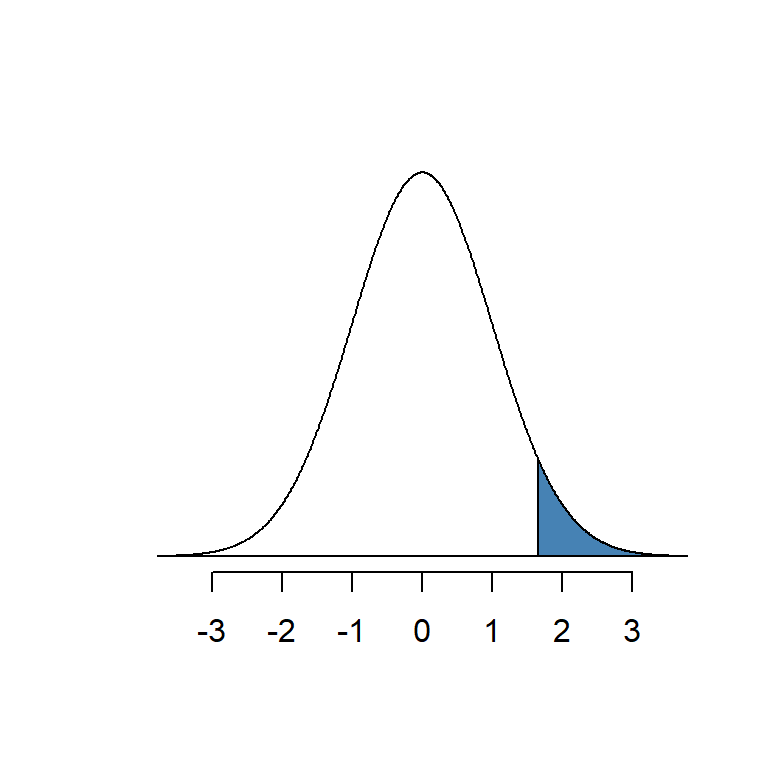
\includegraphics{statformulasbook_files/figure-latex/einsgroesser-fig-1}

\}

\textbackslash caption\{5\%-Verwerfungsbereich für \(\mu\) \textgreater{} Nullwert\}\label{fig:einsgroesser-fig}
\textbackslash end\{figure\}

\begin{enumerate}
\def\labelenumi{\arabic{enumi}.}
\setcounter{enumi}{1}
\tightlist
\item
  Fall
\end{enumerate}

\[H_0: \mu = Nullwert\]
\[H_A: \mu < Nullwert\]

\begin{equation}
  z = \frac{\bar{x}-Nullwert}{SE_{\bar{x}}}
  \label{eq:zonesidedless}
\end{equation}

\(p\)-Wert in \texttt{R} berechnen:

\begin{Shaded}
\begin{Highlighting}[]
\NormalTok{p }\OtherTok{\textless{}{-}} \FunctionTok{pnorm}\NormalTok{(z)}
\end{Highlighting}
\end{Shaded}

\textbackslash begin\{figure\}

\{\centering 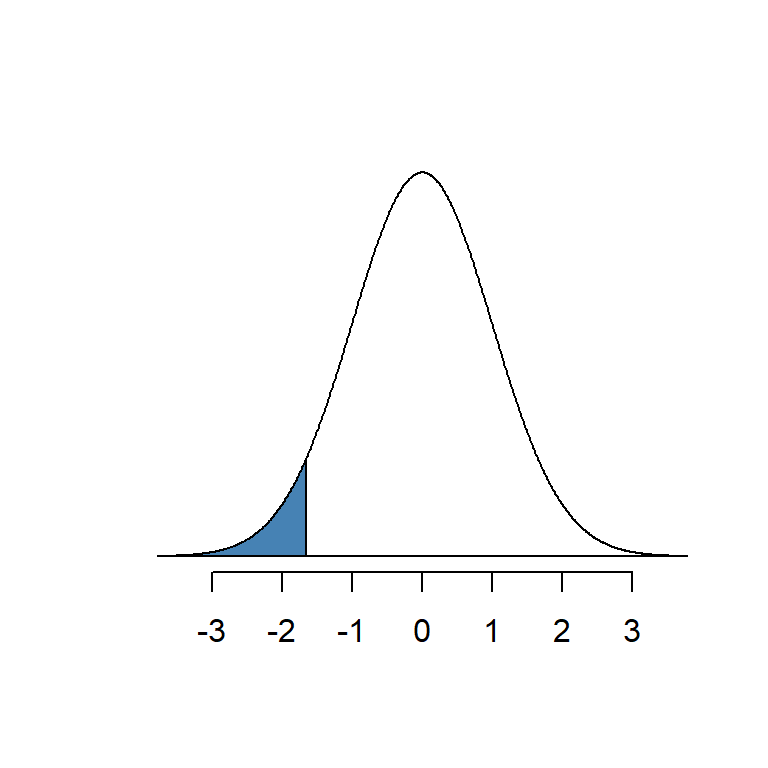
\includegraphics{statformulasbook_files/figure-latex/einskleiner-fig-1}

\}

\textbackslash caption\{5\%-Verwerfungsbereich für \(\mu\) \textless{} Nullwert\}\label{fig:einskleiner-fig}
\textbackslash end\{figure\}

\textbf{Zweiseitiger Hypothesentest anhand von p-Werten}

Zweiseitige Hypothesen sind der Normalfall. Einseitige Hypothesen sollten nur in begründeten Ausnahmefällen formuliert werden.

\[H_0: \mu = Nullwert\]
\[H_A: \mu \neq Nullvalue\]

\begin{equation}
  z = \frac{\bar{x}-Nullwert}{SE_{\bar{x}}}
  \label{eq:ztwosided}
\end{equation}

\(p\)-Wert in \texttt{R} berechnen:

\begin{Shaded}
\begin{Highlighting}[]
\NormalTok{p }\OtherTok{\textless{}{-}} \DecValTok{2} \SpecialCharTok{*} \FunctionTok{pnorm}\NormalTok{(}\FunctionTok{abs}\NormalTok{(z), }\AttributeTok{lower.tail =} \ConstantTok{FALSE}\NormalTok{)}

\CommentTok{\# Alternative}
\NormalTok{p }\OtherTok{\textless{}{-}} \DecValTok{2} \SpecialCharTok{*} \FunctionTok{pnorm}\NormalTok{(}\SpecialCharTok{{-}}\FunctionTok{abs}\NormalTok{(z))}
\end{Highlighting}
\end{Shaded}

\textbackslash begin\{figure\}

\{\centering 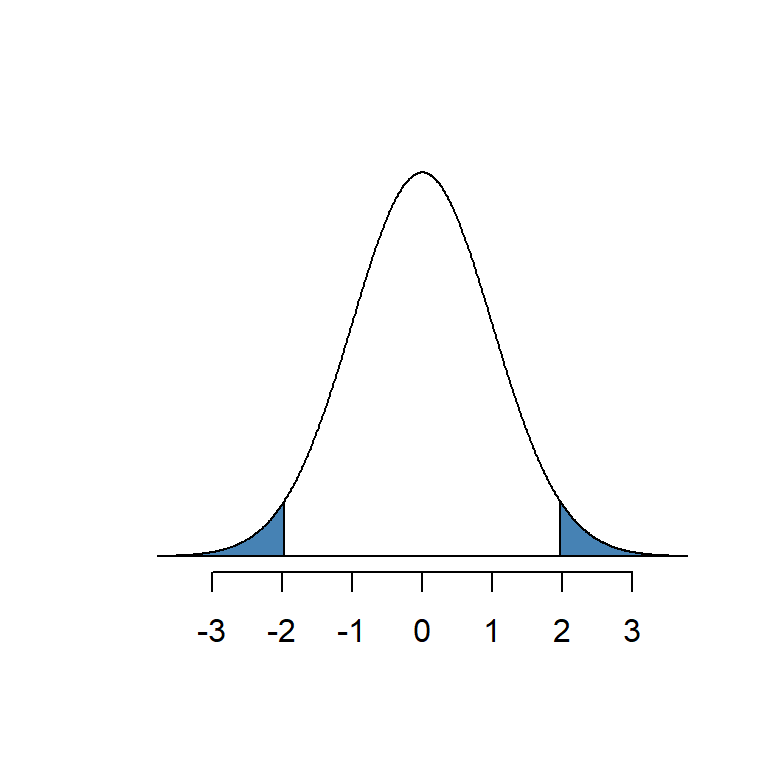
\includegraphics{statformulasbook_files/figure-latex/zweis-fig-1}

\}

\textbackslash caption\{5\%-Verwerfungsbereiche für \(\mu \neq\) Nullwert\}\label{fig:zweis-fig}
\textbackslash end\{figure\}

\hypertarget{entscheidungsfehler}{%
\subsection{Entscheidungsfehler}\label{entscheidungsfehler}}

\begin{itemize}
\tightlist
\item
  Fehler 1. Art: \(H_0\) wird verworfen wenn \(H_0\) wahr ist.\\
\item
  Fehler 2. Art: \(H_0\) wird nicht verworfen wenn \(H_A\) wahr ist.
\end{itemize}

Bei einem Signifikanzniveau \(\alpha = 0.05\) nehmen wir ein Risiko von 5\% in Kauf, einen Fehler 1. Art zu begehen.

\(\alpha:\) Wahrscheinlichkeit, einen Fehler 1. Art zu begehen.\\
\(\beta:\) Wahrscheinlichkeit, einen Fehler 2. Art zu begehen.\\
\(1-\beta:\) Power (Trennschärfe) eines Tests; Wahrscheinlichkeit, für \(H_A\) zu entscheiden, wenn \(H_A\) wahr ist.

\hypertarget{hypothesentests-mit-konfidenzintervallen}{%
\subsection{Hypothesentests mit Konfidenzintervallen}\label{hypothesentests-mit-konfidenzintervallen}}

\begin{itemize}
\tightlist
\item
  Ein zweiseitiger Hypothesentest mit einem Signifikanzniveau \(\alpha\) entspricht einem Konfidenzintervall mit dem Konfidenzniveau \(1-\alpha\).\\
\item
  Ein einseitiger Hypothesentest mit einem Signifikanzniveau \(\alpha\) entspricht einem Vertrauensintervall mit einem Konfidenzniveau von \(1-(2 \times \alpha)\).\\
\item
  Enthält ein 95\% Vertrauensintervall den Nullwert nicht, wird \(H_0\) verworfen.\\
\item
  Enthält ein 95\% Vertrauensintervall den Nullwert, wird \(H_0\) nicht verworfen.
\end{itemize}

\hypertarget{vorgehen-1}{%
\subsection{Vorgehen}\label{vorgehen-1}}

\begin{enumerate}
\def\labelenumi{\arabic{enumi}.}
\tightlist
\item
  Hypothesen \(H_0\) und \(H_A\) formulieren.
\item
  Signifikanzniveau \(\alpha\) festlegen (meist \(\alpha\) = 0.05).
\item
  Voraussetzungen (Normalverteilung, Stichprobenumfang) für Testwahl prüfen.
\item
  (1-\(\alpha\))-Konfidenzintervall für Populationsparameter berechnen.
\item
  Teststatistik berechnen.\\
\item
  \(p\)-Wert für die Teststatisik berechnen.\\
\item
  \(p\)-Wert mit Signifikanzniveau vergleichen und Entscheiden ob man \(H_0\) verwirft oder beibehält.
\item
  Ergebnis in allgemein verständlicher Sprache formulieren.
\end{enumerate}

\hypertarget{inferenz-fuxfcr-quantitative-daten}{%
\chapter{Inferenz für quantitative Daten}\label{inferenz-fuxfcr-quantitative-daten}}

\hypertarget{parametrische-testverfahren}{%
\section{Parametrische Testverfahren}\label{parametrische-testverfahren}}

Parametrische Testverfahren setzen voraus, dass das zu untersuchende Beobachtungsmerkmal aus einer eindeutig definierten Verteilung, meist aus einer Normalverteilung stammt.

\textbf{Übersicht zur Testwahl}

Voraussetzung: Beobachtungsmerkmal stammt aus einer normalverteilten Population.

Eine Stichprobe

\begin{itemize}
\tightlist
\item
  \(n > 30 \rightarrow\) \textbf{z-Test}\\
\item
  \(n \leq 30 \rightarrow\) \textbf{Einstichproben-t-Test}
\end{itemize}

zwei Stichproben

\begin{itemize}
\tightlist
\item
  verbundene (abhängige) Stichproben \(\rightarrow\) \textbf{t-Test für verbundene Stichproben}\\
\item
  unabhängige Stichproben \(\rightarrow\) \textbf{t-Test für unabhängige Stichproben (Welch-Test)}
\end{itemize}

\hypertarget{z-test}{%
\subsection{z-Test}\label{z-test}}

Mit dem \(z\)-Test vergleichen wir den Mittelwert einer Stichprobe mit einem bekannten
Populationsmittelwert (= Nullwert).

\begin{enumerate}
\def\labelenumi{\arabic{enumi}.}
\tightlist
\item
  Hypothesen \(H_0\) und \(H_A\) formulieren.
\end{enumerate}

\begin{itemize}
\tightlist
\item
  \(H_0: \mu = Nullwert\)\\
\item
  \(H_A: \mu \neq Nullwert\)
\end{itemize}

\begin{enumerate}
\def\labelenumi{\arabic{enumi}.}
\setcounter{enumi}{1}
\item
  Signifikanzniveau \(\alpha\) festlegen (meist \(\alpha\) = 0.05).
\item
  Voraussetzungen (Normalverteilung, Stichprobenumfang) für Testwahl prüfen.

  \begin{itemize}
  \tightlist
  \item
    \(n \geq 30\)
  \item
    Zufallsstichprobe\\
  \item
    Beobachtungsmerkmal muss quantitativ und annähernd normalverteilt sein.
  \end{itemize}
\item
  (1-\(\alpha\))-Konfidenzintervall für Populationsparameter berechnen.
\end{enumerate}

\begin{equation}
  CI_{1-\alpha} = \bar{x} \pm z_{\frac{alpha}{2}} \times SE_{\bar{x}}
  \label{eq:CI-ztest}
\end{equation}

\begin{equation}
  SE_{\bar{x}} = \frac{s}{\sqrt{n}}
  \label{eq:se-ztest}
\end{equation}

\begin{Shaded}
\begin{Highlighting}[]
\CommentTok{\# z für Berechnung des CI in R berechnen}
\NormalTok{z }\OtherTok{\textless{}{-}} \FunctionTok{abs}\NormalTok{(}\FunctionTok{qnorm}\NormalTok{(alpha}\SpecialCharTok{/}\DecValTok{2}\NormalTok{))}
\end{Highlighting}
\end{Shaded}

Wenn der Nullwert nicht im (1 - \(\alpha\)) Konfidenzintervall enthalten ist, ist der
Unterschied zwischen \(\mu\) und Nullwert statistisch signifikant.

\begin{enumerate}
\def\labelenumi{\arabic{enumi}.}
\setcounter{enumi}{4}
\tightlist
\item
  Teststatistik berechnen.
\end{enumerate}

\begin{equation}
 z = \frac{\bar{x} - Nullwert}{SE_{\bar{x}}}
  \label{eq:z-ztest}
\end{equation}

\begin{enumerate}
\def\labelenumi{\arabic{enumi}.}
\setcounter{enumi}{5}
\tightlist
\item
  \(p\)-Wert für die Teststatistik berechnen.
\end{enumerate}

\begin{Shaded}
\begin{Highlighting}[]
\CommentTok{\# p{-}Wert für eine zweiseitige Hypothese}
\DecValTok{2} \SpecialCharTok{*}\NormalTok{ (}\DecValTok{1} \SpecialCharTok{{-}} \FunctionTok{pnorm}\NormalTok{(}\FunctionTok{abs}\NormalTok{(z)))}

\CommentTok{\# alternativ}
\DecValTok{2} \SpecialCharTok{*} \FunctionTok{pnorm}\NormalTok{(}\SpecialCharTok{{-}}\FunctionTok{abs}\NormalTok{(z))}
\DecValTok{2} \SpecialCharTok{*} \FunctionTok{pnorm}\NormalTok{(}\FunctionTok{abs}\NormalTok{(z), }\AttributeTok{lower.tail =} \ConstantTok{FALSE}\NormalTok{)}
\end{Highlighting}
\end{Shaded}

\begin{enumerate}
\def\labelenumi{\arabic{enumi}.}
\setcounter{enumi}{6}
\item
  \(p\)-Wert mit Signifikanzniveau vergleichen und Entscheiden ob man \(H_0\) verwirft oder beibehält.\\
  Ist der \(p\)-Wert kleiner als das Signifikanzniveau \(\alpha\), wird die \(H_0\) zu Gunsten der \(H_A\) verworfen.
\item
  Ergebnis in allgemein verständlicher Sprache formulieren.
\end{enumerate}

Beispiel: Bei 30 Personen wurde der Effekt eines Blutdruckmedikaments getestet. Der Hersteller gibt an, dass das Medikament den systolischen Blutdruck im Durchschnitt um 5 mmHg senkt. Der Effekt auf den systolischen Blutdruck wurde in der Variablen \texttt{BDsys} gespeichert.

\begin{Shaded}
\begin{Highlighting}[]
\FunctionTok{set.seed}\NormalTok{(}\DecValTok{1}\NormalTok{)}
\NormalTok{BDsys }\OtherTok{\textless{}{-}} \FunctionTok{rnorm}\NormalTok{(}\DecValTok{30}\NormalTok{, }\AttributeTok{mean =} \SpecialCharTok{{-}}\DecValTok{6}\NormalTok{, }\AttributeTok{sd =} \DecValTok{4}\NormalTok{)  }\CommentTok{\# simulierte Daten generieren  }
\NormalTok{alpha }\OtherTok{\textless{}{-}} \FloatTok{0.05}                          \CommentTok{\# Signifikanzniveau festlegen}

\CommentTok{\# CI berechnen  }
\NormalTok{mean.BDsys }\OtherTok{\textless{}{-}} \FunctionTok{mean}\NormalTok{(BDsys)              }\CommentTok{\# Mittelwert für BDsys}
\NormalTok{sd.BDsys }\OtherTok{\textless{}{-}} \FunctionTok{sd}\NormalTok{(BDsys)                  }\CommentTok{\# Standardabweichung für BDsys}
\NormalTok{n.BDsys }\OtherTok{\textless{}{-}} \FunctionTok{length}\NormalTok{(BDsys)               }\CommentTok{\# Stichprobenumfang für BDsys}
\NormalTok{SE.BDsys }\OtherTok{\textless{}{-}}\NormalTok{ sd.BDsys }\SpecialCharTok{/} \FunctionTok{sqrt}\NormalTok{(n.BDsys)   }\CommentTok{\# SE für Mittelwert von BDsys    }
\NormalTok{z.CI }\OtherTok{\textless{}{-}} \FunctionTok{abs}\NormalTok{(}\FunctionTok{qnorm}\NormalTok{(alpha }\SpecialCharTok{/} \DecValTok{2}\NormalTok{))          }\CommentTok{\# z{-}Wert}
\NormalTok{CI }\OtherTok{\textless{}{-}}\NormalTok{ mean.BDsys }\SpecialCharTok{+} \FunctionTok{c}\NormalTok{(}\SpecialCharTok{{-}}\DecValTok{1}\NormalTok{, }\DecValTok{1}\NormalTok{) }\SpecialCharTok{*}\NormalTok{ z.CI }\SpecialCharTok{*}\NormalTok{ SE.BDsys  }\CommentTok{\#  Grenzen für CI berechnen}
\NormalTok{CI }\OtherTok{\textless{}{-}} \FunctionTok{round}\NormalTok{(CI, }\DecValTok{3}\NormalTok{)                     }\CommentTok{\# Werte für CI auf 3 Stellen runden}
\NormalTok{CI.output }\OtherTok{\textless{}{-}} \FunctionTok{paste}\NormalTok{((}\DecValTok{1} \SpecialCharTok{{-}}\NormalTok{ alpha) }\SpecialCharTok{*} \DecValTok{100}\NormalTok{, }\StringTok{"\%{-}CI ["}\NormalTok{, CI[}\DecValTok{1}\NormalTok{], }\StringTok{", "}\NormalTok{, CI[}\DecValTok{2}\NormalTok{], }\StringTok{"]"}\NormalTok{, }\AttributeTok{sep =} \StringTok{""}\NormalTok{)}
\FunctionTok{print}\NormalTok{(CI.output)                       }\CommentTok{\# CI ausgeben}
\end{Highlighting}
\end{Shaded}

\begin{verbatim}
## [1] "95%-CI [-6.993, -4.347]"
\end{verbatim}

\begin{Shaded}
\begin{Highlighting}[]
\CommentTok{\# Teststatistik berechnen}
\NormalTok{nullvalue }\OtherTok{\textless{}{-}} \SpecialCharTok{{-}}\DecValTok{5}                        \CommentTok{\# Nullwert eingeben}
\NormalTok{z }\OtherTok{\textless{}{-}}\NormalTok{ (mean.BDsys }\SpecialCharTok{{-}}\NormalTok{ nullvalue)}\SpecialCharTok{/}\NormalTok{SE.BDsys }\CommentTok{\# z{-}Wert berechnen}
\NormalTok{p }\OtherTok{\textless{}{-}} \DecValTok{2} \SpecialCharTok{*} \FunctionTok{pnorm}\NormalTok{(}\SpecialCharTok{{-}}\FunctionTok{abs}\NormalTok{(z))                }\CommentTok{\# p{-}Wert für z berechnen  (zweiseitig) }
\NormalTok{z }\OtherTok{\textless{}{-}} \FunctionTok{round}\NormalTok{(z, }\DecValTok{3}\NormalTok{)                       }\CommentTok{\# z auf 3 Stellen runden}
\NormalTok{p }\OtherTok{\textless{}{-}} \FunctionTok{round}\NormalTok{(p, }\DecValTok{4}\NormalTok{)                       }\CommentTok{\# p{-}Wert auf 4 Stellen runden}
\NormalTok{result }\OtherTok{\textless{}{-}} \FunctionTok{paste}\NormalTok{(}\StringTok{"z = "}\NormalTok{, z, }\StringTok{", p = "}\NormalTok{, p, }\AttributeTok{sep =} \StringTok{""}\NormalTok{)  }
\FunctionTok{print}\NormalTok{(result)}
\end{Highlighting}
\end{Shaded}

\begin{verbatim}
## [1] "z = -0.993, p = 0.3207"
\end{verbatim}

Ergebnis in allgemein verständlicher Sprache formulieren: Die Einnahme des Blutdrucksenkers reduziert den systolischen Blutdruck im Durchschnitt um -5.67, 95\%-CI {[}-6.993, -4.347{]} mmHg. Der vom Hersteller angegebene Wert von durchschnittlich -5 mmHg ist in diesem 95\%-Konfidenzintervall enthalten und es liegt keine Evidenz gegen die Nullhypothese (\(H_0: \mu = -5\)) vor, \(z\) = -0.993, \(p\) = 0.3207.

\textbf{Hinweis:} Für den \(z\)-Test existiert keine Funktion in \texttt{R-base}. Zum Überprüfen der
Ergebnisse kann die Funkion \texttt{z.test()} aus dem Package \texttt{BSDA} verwendet werden.

\begin{Shaded}
\begin{Highlighting}[]
\FunctionTok{install.packages}\NormalTok{(}\StringTok{"BSDA"}\NormalTok{)}
\FunctionTok{library}\NormalTok{(BSDA)}
\FunctionTok{z.test}\NormalTok{()                               }\CommentTok{\# für Beschreibung ?z.test eingeben}
\end{Highlighting}
\end{Shaded}

\hypertarget{einstichproben-t-test}{%
\subsection{\texorpdfstring{Einstichproben-\(t\)-Test}{Einstichproben-t-Test}}\label{einstichproben-t-test}}

Wie beim \(z\)-Test vergleichen wir den Mittelwert einer Stichprobe mit einem bekannten Populationsmittelwert (= Nullwert). Bei kleinen Stichproben (\(n < 30\)) kann der \(z\)-Test allerdings nicht angewendet werden und wir verwenden den Einstichproben-\(t\)-Test.

\textbf{Merke: Statistikprogramme wie \texttt{R} verwenden immer den \(t\)-Test.}

\begin{enumerate}
\def\labelenumi{\arabic{enumi}.}
\tightlist
\item
  Hypothesen \(H_0\) und \(H_A\) formulieren.
\end{enumerate}

\begin{itemize}
\tightlist
\item
  \(H_0: \mu = Nullwert\)\\
\item
  \(H_A: \mu \neq Nullwert\)
\end{itemize}

\begin{enumerate}
\def\labelenumi{\arabic{enumi}.}
\setcounter{enumi}{1}
\item
  Signifikanzniveau \(\alpha\) festlegen (meist \(\alpha\) = 0.05).
\item
  Voraussetzungen (Normalverteilung, Stichprobenumfang) für Testwahl prüfen.

  \begin{itemize}
  \tightlist
  \item
    Zufallsstichprobe\\
  \item
    Beobachtungsmerkmal muss quantitativ und annähernd normalverteilt sein.
  \end{itemize}
\item
  (1-\(\alpha\))-Konfidenzintervall für Populationsparameter berechnen.
\end{enumerate}

\begin{equation}
  CI_{1-\alpha} = \bar{x} \pm t_{\frac{\alpha}{2},df} \times SE_{\bar{x}}
  \label{eq:CI-ttest}
\end{equation}

\begin{equation}
  SE_{\bar{x}} = \frac{s}{\sqrt{n}}, ~~ df = n-1
  \label{eq:se-ttest}
\end{equation}

\begin{Shaded}
\begin{Highlighting}[]
\CommentTok{\# t für Berechnung des CI in R berechnen}
\NormalTok{t }\OtherTok{\textless{}{-}} \FunctionTok{abs}\NormalTok{(}\FunctionTok{qt}\NormalTok{(alpha}\SpecialCharTok{/}\DecValTok{2}\NormalTok{), }\AttributeTok{df =}\NormalTok{ n }\SpecialCharTok{{-}} \DecValTok{1}\NormalTok{)}
\end{Highlighting}
\end{Shaded}

Wenn der Nullwert nicht im (1 - \(\alpha\)) Konfidenzintervall enthalten ist, ist der
Unterschied zwischen \(\mu\) und Nullwert statistisch signifikant.

\begin{enumerate}
\def\labelenumi{\arabic{enumi}.}
\setcounter{enumi}{4}
\tightlist
\item
  Teststatistik berechnen.
\end{enumerate}

\begin{equation}
  t = \frac{\bar{x} - Nullwert}{SE_{\bar{x}}}
  \label{eq:t-ztest}
\end{equation}

\begin{enumerate}
\def\labelenumi{\arabic{enumi}.}
\setcounter{enumi}{5}
\tightlist
\item
  \(p\)-Wert für die Teststatistik berechnen.
\end{enumerate}

\begin{Shaded}
\begin{Highlighting}[]
\CommentTok{\# p{-}Wert für eine zweiseitige Hypothese}
\DecValTok{2} \SpecialCharTok{*}\NormalTok{ (}\DecValTok{1} \SpecialCharTok{{-}} \FunctionTok{pt}\NormalTok{(}\FunctionTok{abs}\NormalTok{(t), }\AttributeTok{df =}\NormalTok{ n }\SpecialCharTok{{-}} \DecValTok{1}\NormalTok{ ))}

\CommentTok{\# alternativ}
\DecValTok{2} \SpecialCharTok{*} \FunctionTok{pt}\NormalTok{(}\SpecialCharTok{{-}}\FunctionTok{abs}\NormalTok{(t), }\AttributeTok{df =}\NormalTok{ n }\SpecialCharTok{{-}} \DecValTok{1}\NormalTok{)}
\DecValTok{2} \SpecialCharTok{*} \FunctionTok{pt}\NormalTok{(}\FunctionTok{abs}\NormalTok{(t), , }\AttributeTok{df =}\NormalTok{ n }\SpecialCharTok{{-}} \DecValTok{1}\NormalTok{, }\AttributeTok{lower.tail =} \ConstantTok{FALSE}\NormalTok{)}
\end{Highlighting}
\end{Shaded}

\begin{enumerate}
\def\labelenumi{\arabic{enumi}.}
\setcounter{enumi}{6}
\item
  \(p\)-Wert mit Signifikanzniveau vergleichen und Entscheiden ob man \(H_0\) verwirft oder beibehält.\\
  Ist der \(p\)-Wert kleiner als das Signifikanzniveau \(\alpha\), wird die \(H_0\) zu Gunsten der \(H_A\) verworfen.
\item
  Ergebnis in allgemein verständlicher Sprache formulieren.
\end{enumerate}

Beispiel: Bei 12 Personen wurde der Effekt eines Blutdruckmedikaments getestet. Der Hersteller gibt an, dass das Medikament den systolischen Blutdruck im Durchschnitt um 5 mmHg senkt. Der Effekt auf den systolischen Blutdruck wurde in der Variablen \texttt{BDsys} gespeichert.

\begin{Shaded}
\begin{Highlighting}[]
\FunctionTok{set.seed}\NormalTok{(}\DecValTok{1}\NormalTok{)}
\NormalTok{BDsys }\OtherTok{\textless{}{-}} \FunctionTok{rnorm}\NormalTok{(}\DecValTok{12}\NormalTok{, }\AttributeTok{mean =} \SpecialCharTok{{-}}\DecValTok{6}\NormalTok{, }\AttributeTok{sd =} \DecValTok{4}\NormalTok{)  }\CommentTok{\# simulierte Daten generieren  }
\NormalTok{alpha }\OtherTok{\textless{}{-}} \FloatTok{0.05}                          \CommentTok{\# Signifikanzniveau festlegen}

\CommentTok{\# CI berechnen  }
\NormalTok{mean.BDsys }\OtherTok{\textless{}{-}} \FunctionTok{mean}\NormalTok{(BDsys)              }\CommentTok{\# Mittelwert für BDsys}
\NormalTok{sd.BDsys }\OtherTok{\textless{}{-}} \FunctionTok{sd}\NormalTok{(BDsys)                  }\CommentTok{\# Standardabweichung für BDsys}
\NormalTok{n.BDsys }\OtherTok{\textless{}{-}} \FunctionTok{length}\NormalTok{(BDsys)               }\CommentTok{\# Stichprobenumfang für BDsys}
\NormalTok{SE.BDsys }\OtherTok{\textless{}{-}}\NormalTok{ sd.BDsys }\SpecialCharTok{/} \FunctionTok{sqrt}\NormalTok{(n.BDsys)   }\CommentTok{\# SE für Mittelwert von BDsys    }
\NormalTok{t.CI }\OtherTok{\textless{}{-}} \FunctionTok{abs}\NormalTok{(}\FunctionTok{qt}\NormalTok{(alpha }\SpecialCharTok{/} \DecValTok{2}\NormalTok{, }\AttributeTok{df =}\NormalTok{ n.BDsys }\SpecialCharTok{{-}} \DecValTok{1}\NormalTok{))  }\CommentTok{\# t{-}Wert}
\NormalTok{CI }\OtherTok{\textless{}{-}}\NormalTok{ mean.BDsys }\SpecialCharTok{+} \FunctionTok{c}\NormalTok{(}\SpecialCharTok{{-}}\DecValTok{1}\NormalTok{, }\DecValTok{1}\NormalTok{) }\SpecialCharTok{*}\NormalTok{ t.CI }\SpecialCharTok{*}\NormalTok{ SE.BDsys  }\CommentTok{\#  Grenzen für CI berechnen}
\NormalTok{CI }\OtherTok{\textless{}{-}} \FunctionTok{round}\NormalTok{(CI, }\DecValTok{3}\NormalTok{)                     }\CommentTok{\# Werte für CI auf 3 Stellen runden}
\NormalTok{CI.output }\OtherTok{\textless{}{-}} \FunctionTok{paste}\NormalTok{((}\DecValTok{1} \SpecialCharTok{{-}}\NormalTok{ alpha) }\SpecialCharTok{*} \DecValTok{100}\NormalTok{, }\StringTok{"\%{-}CI ["}\NormalTok{, CI[}\DecValTok{1}\NormalTok{], }\StringTok{", "}\NormalTok{, CI[}\DecValTok{2}\NormalTok{], }\StringTok{"]"}\NormalTok{, }\AttributeTok{sep =} \StringTok{""}\NormalTok{)}
\FunctionTok{print}\NormalTok{(CI.output)                       }\CommentTok{\# CI ausgeben}
\end{Highlighting}
\end{Shaded}

\begin{verbatim}
## [1] "95%-CI [-6.986, -2.865]"
\end{verbatim}

\begin{Shaded}
\begin{Highlighting}[]
\CommentTok{\# Teststatistik berechnen}
\NormalTok{nullvalue }\OtherTok{\textless{}{-}} \SpecialCharTok{{-}}\DecValTok{5}                        \CommentTok{\# Nullwert eingeben}
\NormalTok{t }\OtherTok{\textless{}{-}}\NormalTok{ (mean.BDsys }\SpecialCharTok{{-}}\NormalTok{ nullvalue)}\SpecialCharTok{/}\NormalTok{SE.BDsys }\CommentTok{\# z{-}Wert berechnen}
\NormalTok{p }\OtherTok{\textless{}{-}} \DecValTok{2} \SpecialCharTok{*} \FunctionTok{pt}\NormalTok{(}\SpecialCharTok{{-}}\FunctionTok{abs}\NormalTok{(t), }\AttributeTok{df =}\NormalTok{ n.BDsys }\SpecialCharTok{{-}} \DecValTok{1}\NormalTok{) }\CommentTok{\# p{-}Wert für z berechnen  (zweiseitig) }
\NormalTok{t }\OtherTok{\textless{}{-}} \FunctionTok{round}\NormalTok{(t, }\DecValTok{4}\NormalTok{)                       }\CommentTok{\# z auf 3 Stellen runden}
\NormalTok{p }\OtherTok{\textless{}{-}} \FunctionTok{round}\NormalTok{(p, }\DecValTok{4}\NormalTok{)                       }\CommentTok{\# p{-}Wert auf 4 Stellen runden}
\NormalTok{result }\OtherTok{\textless{}{-}} \FunctionTok{paste}\NormalTok{(}\StringTok{"t = "}\NormalTok{, t, }\StringTok{", p = "}\NormalTok{, p, }\AttributeTok{sep =} \StringTok{""}\NormalTok{)  }
\FunctionTok{print}\NormalTok{(result)}
\end{Highlighting}
\end{Shaded}

\begin{verbatim}
## [1] "t = 0.0796, p = 0.938"
\end{verbatim}

Ergebnis in allgemein verständlicher Sprache formulieren: Die Einnahme des Blutdrucksenkers reduziert den systolischen Blutdruck im Durchschnitt um -4.925, 95\%-CI {[}-6.986, -2.865{]} mmHg. Der vom Hersteller angegebene Wert von durchschnittlich -5 mmHg ist in diesem 95\%-Konfidenzintervall enthalten und es liegt keine Evidenz gegen die Nullhypothese (\(H_0: \mu = -5\)) vor, \(t\) = 0.0796, \(df\) = 11, \(p\) = 0.938.

Einfacher geht es mit der \texttt{R}-Funktion \texttt{t.test()}.

\begin{Shaded}
\begin{Highlighting}[]
\FunctionTok{t.test}\NormalTok{(BDsys, }\AttributeTok{mu =} \SpecialCharTok{{-}}\DecValTok{5}\NormalTok{)}
\end{Highlighting}
\end{Shaded}

\begin{verbatim}
## 
##  One Sample t-test
## 
## data:  BDsys
## t = 0.08, df = 11, p-value = 0.9
## alternative hypothesis: true mean is not equal to -5
## 95 percent confidence interval:
##  -6.986 -2.865
## sample estimates:
## mean of x 
##    -4.925
\end{verbatim}

\hypertarget{t-test-fuxfcr-verbundene-stichproben}{%
\subsection{t-Test für verbundene Stichproben}\label{t-test-fuxfcr-verbundene-stichproben}}

Bei abhängigen Stichproben wird davon ausgegangen, dass die Messwerte in ``Paaren'' vorliegen, z.B.

\begin{itemize}
\tightlist
\item
  Gleiche Beobachtungseinheiten: Vorher-Nachher-Messungen, Messwiederholungen\\
\item
  Unterschiedliche Beobachtungseinheiten (jedoch voneinander abhängig): Zwillingsstudien, Partner, matched pairs.
\end{itemize}

Parameter: \(\mu_{\Delta}\) = Mittelwert der paarweisen Differenzen in der Population\\
Punktschätzer: \(\bar{x}_{\Delta}\) = Mittelwert der paarweisen Differenzen in der Stichprobe\\
Teststatistik: \(t\)

\begin{enumerate}
\def\labelenumi{\arabic{enumi}.}
\tightlist
\item
  Hypothesen \(H_0\) und \(H_A\) formulieren.
\end{enumerate}

\begin{itemize}
\tightlist
\item
  \(H_0: \mu_{\Delta} = 0\)\\
\item
  \(H_A: \mu_{\Delta} \neq 0\) (zweiseitige \(H_A\))
\end{itemize}

\begin{enumerate}
\def\labelenumi{\arabic{enumi}.}
\setcounter{enumi}{1}
\item
  Signifikanzniveau \(\alpha\) festlegen (meist \(\alpha\) = 0.05).
\item
  Voraussetzungen (Normalverteilung, Stichprobenumfang) für Testwahl prüfen.
\end{enumerate}

\begin{itemize}
\tightlist
\item
  Zufallsstichprobe\\
\item
  Paarweise Differenzen sind annähernd normalverteilt.\\
\item
  \(n \geq 12\) oder grösser bei stark schiefen Verteilungen
\end{itemize}

\begin{enumerate}
\def\labelenumi{\arabic{enumi}.}
\setcounter{enumi}{3}
\tightlist
\item
  (1-\(\alpha\))-Konfidenzintervall für Populationsparameter berechnen.
\end{enumerate}

\begin{equation}
  CI_{1-\alpha} = \bar{x}_{\Delta} \pm t_{\frac{\alpha}{2}, df} \times SE_{\bar{x}_{\Delta}}
  \label{eq:CI-tpaired}
\end{equation}

\begin{equation}
  SE_{\bar{x}_{\Delta}} = \frac{s_{\Delta}}{\sqrt{n}}, ~~ df = n-1
  \label{eq:se-tpaired}
\end{equation}

\begin{Shaded}
\begin{Highlighting}[]
\CommentTok{\# t für Berechnung des CI in R berechnen}
\NormalTok{t }\OtherTok{\textless{}{-}} \FunctionTok{abs}\NormalTok{(}\FunctionTok{qt}\NormalTok{(alpha}\SpecialCharTok{/}\DecValTok{2}\NormalTok{), }\AttributeTok{df =}\NormalTok{ n }\SpecialCharTok{{-}} \DecValTok{1}\NormalTok{)}
\end{Highlighting}
\end{Shaded}

\begin{enumerate}
\def\labelenumi{\arabic{enumi}.}
\setcounter{enumi}{4}
\tightlist
\item
  Teststatistik berechnen.
\end{enumerate}

\begin{equation}
  t = \frac{\bar{x}_{\Delta} - 0}{SE_{\bar{x}_{\Delta}}}
  \label{eq:t-paired}
\end{equation}

\begin{enumerate}
\def\labelenumi{\arabic{enumi}.}
\setcounter{enumi}{5}
\tightlist
\item
  \(p\)-Wert für die Teststatisik berechnen.
\end{enumerate}

\begin{Shaded}
\begin{Highlighting}[]
\CommentTok{\# p{-}Wert für eine zweiseitige Hypothese}
\DecValTok{2} \SpecialCharTok{*}\NormalTok{ (}\DecValTok{1} \SpecialCharTok{{-}} \FunctionTok{pt}\NormalTok{(}\FunctionTok{abs}\NormalTok{(t), }\AttributeTok{df =}\NormalTok{ n }\SpecialCharTok{{-}} \DecValTok{1}\NormalTok{ ))}

\CommentTok{\# alternativ}
\DecValTok{2} \SpecialCharTok{*} \FunctionTok{pt}\NormalTok{(}\SpecialCharTok{{-}}\FunctionTok{abs}\NormalTok{(t), }\AttributeTok{df =}\NormalTok{ n }\SpecialCharTok{{-}} \DecValTok{1}\NormalTok{)}
\DecValTok{2} \SpecialCharTok{*} \FunctionTok{pt}\NormalTok{(}\FunctionTok{abs}\NormalTok{(t), , }\AttributeTok{df =}\NormalTok{ n }\SpecialCharTok{{-}} \DecValTok{1}\NormalTok{, }\AttributeTok{lower.tail =} \ConstantTok{FALSE}\NormalTok{)}
\end{Highlighting}
\end{Shaded}

\begin{enumerate}
\def\labelenumi{\arabic{enumi}.}
\setcounter{enumi}{6}
\item
  \(p\)-Wert mit Signifikanzniveau vergleichen und Entscheiden ob man \(H_0\) verwirft oder beibehält.\\
  Ist der \(p\)-Wert kleiner als das Signifikanzniveau \(\alpha\), wird die \(H_0\) zu Gunsten der \(H_A\) verworfen.
\item
  Ergebnis in allgemein verständlicher Sprache formulieren.
\end{enumerate}

Beispiel: Körpergewicht in kg für 17 Probandinnen vor und nach einer Anorexie Therapie. Hat die Therapie einen signifikanten Effekt?

\begin{Shaded}
\begin{Highlighting}[]
\DocumentationTok{\#\# create dataset (data extracted \& converted from package PairedData::Anorexia)}
\NormalTok{anorexia }\OtherTok{\textless{}{-}} \FunctionTok{data.frame}\NormalTok{(}
  \AttributeTok{id =} \FunctionTok{seq}\NormalTok{(}\AttributeTok{from =} \DecValTok{1}\NormalTok{, }\AttributeTok{to =} \DecValTok{17}\NormalTok{, }\AttributeTok{by =} \DecValTok{1}\NormalTok{),}
  \AttributeTok{vor =} \FunctionTok{c}\NormalTok{(}\FloatTok{38.0}\NormalTok{, }\FloatTok{37.8}\NormalTok{, }\FloatTok{39.0}\NormalTok{, }\FloatTok{37.4}\NormalTok{, }\FloatTok{39.3}\NormalTok{, }\FloatTok{36.1}\NormalTok{, }\FloatTok{34.9}\NormalTok{, }\FloatTok{42.7}\NormalTok{, }\FloatTok{33.3}\NormalTok{, }\FloatTok{36.5}\NormalTok{, }\FloatTok{37.0}\NormalTok{, }\FloatTok{37.2}\NormalTok{, }\FloatTok{35.2}\NormalTok{, }\FloatTok{37.9}\NormalTok{, }\FloatTok{40.8}\NormalTok{, }\FloatTok{39.0}\NormalTok{, }\FloatTok{39.6}\NormalTok{),}
  \AttributeTok{nach =} \FunctionTok{c}\NormalTok{(}\FloatTok{43.2}\NormalTok{, }\FloatTok{42.8}\NormalTok{, }\FloatTok{41.5}\NormalTok{, }\FloatTok{41.7}\NormalTok{, }\FloatTok{45.5}\NormalTok{, }\FloatTok{34.8}\NormalTok{, }\FloatTok{34.8}\NormalTok{, }\FloatTok{46.1}\NormalTok{, }\FloatTok{43.0}\NormalTok{, }\FloatTok{34.1}\NormalTok{, }\FloatTok{35.3}\NormalTok{, }\FloatTok{43.3}\NormalTok{, }\FloatTok{41.1}\NormalTok{, }\FloatTok{42.0}\NormalTok{, }\FloatTok{42.5}\NormalTok{, }\FloatTok{41.6}\NormalTok{, }\FloatTok{44.5}\NormalTok{)}
\NormalTok{)}

\CommentTok{\# erste 6 Beobachtungseinheiten im Datensatz anzeigen}
\FunctionTok{head}\NormalTok{(anorexia)}
\end{Highlighting}
\end{Shaded}

\begin{verbatim}
##   id  vor nach
## 1  1 38.0 43.2
## 2  2 37.8 42.8
## 3  3 39.0 41.5
## 4  4 37.4 41.7
## 5  5 39.3 45.5
## 6  6 36.1 34.8
\end{verbatim}

\begin{Shaded}
\begin{Highlighting}[]
\CommentTok{\# paarweise Differenzen berechnen und in Variable anorexia$diff speichern}
\NormalTok{anorexia}\SpecialCharTok{$}\NormalTok{diff }\OtherTok{\textless{}{-}}\NormalTok{ anorexia}\SpecialCharTok{$}\NormalTok{nach }\SpecialCharTok{{-}}\NormalTok{ anorexia}\SpecialCharTok{$}\NormalTok{vor}
\FunctionTok{head}\NormalTok{(anorexia)}
\end{Highlighting}
\end{Shaded}

\begin{verbatim}
##   id  vor nach diff
## 1  1 38.0 43.2  5.2
## 2  2 37.8 42.8  5.0
## 3  3 39.0 41.5  2.5
## 4  4 37.4 41.7  4.3
## 5  5 39.3 45.5  6.2
## 6  6 36.1 34.8 -1.3
\end{verbatim}

\begin{Shaded}
\begin{Highlighting}[]
\DocumentationTok{\#\# Verteilung der paarweisen Differenzen prüfen {-}{-}{-}{-}{-}{-}{-}{-}{-}{-}{-}{-}{-}{-}{-}{-}{-}{-}{-}{-}{-}{-}{-}{-}{-}{-}{-}{-}{-}{-}{-}{-}}
\FunctionTok{qqnorm}\NormalTok{(anorexia}\SpecialCharTok{$}\NormalTok{diff)              }\CommentTok{\# QQ{-}Plot erstellen }
\FunctionTok{qqline}\NormalTok{(anorexia}\SpecialCharTok{$}\NormalTok{diff)}
\end{Highlighting}
\end{Shaded}

\begin{center}\includegraphics{statformulasbook_files/figure-latex/unnamed-chunk-22-1} \end{center}

\begin{Shaded}
\begin{Highlighting}[]
\DocumentationTok{\#\# CI für anorexia$diff berechnen {-}{-}{-}{-}{-}{-}{-}{-}{-}{-}{-}{-}{-}{-}{-}{-}{-}{-}{-}{-}{-}{-}{-}{-}{-}{-}{-}{-}{-}{-}{-}{-}{-}{-}{-}{-}{-}{-}{-}{-}{-}{-}{-}{-}{-}{-}}
\NormalTok{alpha }\OtherTok{\textless{}{-}} \FloatTok{0.05}                      \CommentTok{\# Signifikanzniveau festlegen  }
\NormalTok{mean.diff }\OtherTok{\textless{}{-}} \FunctionTok{mean}\NormalTok{(anorexia}\SpecialCharTok{$}\NormalTok{diff)   }\CommentTok{\# Mittelwert der paarweisen Differenzen}
\NormalTok{sd.diff }\OtherTok{\textless{}{-}} \FunctionTok{sd}\NormalTok{(anorexia}\SpecialCharTok{$}\NormalTok{diff)       }\CommentTok{\# Standardabweichung der paarweisen Differenzen}
\NormalTok{n.diff }\OtherTok{\textless{}{-}} \FunctionTok{length}\NormalTok{(anorexia}\SpecialCharTok{$}\NormalTok{diff)    }\CommentTok{\# Stichprobenumfang ermitteln}
\NormalTok{SE.diff }\OtherTok{\textless{}{-}}\NormalTok{ sd.diff}\SpecialCharTok{/}\FunctionTok{sqrt}\NormalTok{(n.diff)    }\CommentTok{\# Standardfehler berechnen  }
\NormalTok{t.CI }\OtherTok{\textless{}{-}} \FunctionTok{abs}\NormalTok{(}\FunctionTok{qt}\NormalTok{(alpha }\SpecialCharTok{/} \DecValTok{2}\NormalTok{, }\AttributeTok{df =}\NormalTok{ n.diff }\SpecialCharTok{{-}} \DecValTok{1}\NormalTok{)) }\CommentTok{\# t für CI{-}Berechnung bestimmen  }
\NormalTok{CI.diff }\OtherTok{\textless{}{-}}\NormalTok{ mean.diff }\SpecialCharTok{+} \FunctionTok{c}\NormalTok{(}\SpecialCharTok{{-}}\DecValTok{1}\NormalTok{, }\DecValTok{1}\NormalTok{) }\SpecialCharTok{*}\NormalTok{ t.CI }\SpecialCharTok{*}\NormalTok{ SE.diff }\CommentTok{\# CI Grenzen berechnen  }
\NormalTok{CI.diff }\OtherTok{\textless{}{-}} \FunctionTok{round}\NormalTok{(CI.diff, }\DecValTok{3}\NormalTok{)                  }\CommentTok{\# CI{-}Grenzen auf drei Stellen runden}
\NormalTok{CI.output }\OtherTok{\textless{}{-}} \FunctionTok{paste}\NormalTok{((}\DecValTok{1} \SpecialCharTok{{-}}\NormalTok{ alpha) }\SpecialCharTok{*} \DecValTok{100}\NormalTok{, }\StringTok{"\%{-}CI ["}\NormalTok{, CI.diff[}\DecValTok{1}\NormalTok{], }\StringTok{", "}\NormalTok{, CI.diff[}\DecValTok{2}\NormalTok{], }\StringTok{"]"}\NormalTok{)}
\NormalTok{CI.output}
\end{Highlighting}
\end{Shaded}

\begin{verbatim}
## [1] "95 %-CI [ 1.631 ,  4.969 ]"
\end{verbatim}

\begin{Shaded}
\begin{Highlighting}[]
\DocumentationTok{\#\# p{-}Wert bestimmen}
\NormalTok{t }\OtherTok{\textless{}{-}}\NormalTok{ (mean.diff }\SpecialCharTok{{-}} \DecValTok{0}\NormalTok{) }\SpecialCharTok{/}\NormalTok{ SE.diff}
\NormalTok{p }\OtherTok{\textless{}{-}} \DecValTok{2} \SpecialCharTok{*} \FunctionTok{pt}\NormalTok{(}\SpecialCharTok{{-}}\FunctionTok{abs}\NormalTok{(t), }\AttributeTok{df =}\NormalTok{ n.diff }\SpecialCharTok{{-}} \DecValTok{1}\NormalTok{)}
\NormalTok{t }\OtherTok{\textless{}{-}} \FunctionTok{round}\NormalTok{(t, }\DecValTok{4}\NormalTok{)}
\NormalTok{p }\OtherTok{\textless{}{-}} \FunctionTok{round}\NormalTok{(p, }\DecValTok{4}\NormalTok{)}
\NormalTok{result }\OtherTok{\textless{}{-}} \FunctionTok{paste}\NormalTok{(}\StringTok{"t = "}\NormalTok{, t, }\StringTok{", p = "}\NormalTok{, p, }\AttributeTok{sep =} \StringTok{""}\NormalTok{)  }
\FunctionTok{print}\NormalTok{(result)}
\end{Highlighting}
\end{Shaded}

\begin{verbatim}
## [1] "t = 4.1917, p = 0.0007"
\end{verbatim}

Ergebnis in allgemein verständlicher Sprache formulieren: Die Therapie führt bei anorektischen Patientinnen im Durchschnitt zu einer signifikanten Gewichtszunahme von 3.3 kg 95 \%-CI {[} 1.631 , 4.969 {]}, \(t\) = 4.1917, \(df\) = 16, \(p\) = 0.0007

Einfacher geht es mit der \texttt{R}-Funktion \texttt{t.test()}.

\begin{Shaded}
\begin{Highlighting}[]
\FunctionTok{t.test}\NormalTok{(anorexia}\SpecialCharTok{$}\NormalTok{nach, anorexia}\SpecialCharTok{$}\NormalTok{vor, }\AttributeTok{paired =} \ConstantTok{TRUE}\NormalTok{)}
\end{Highlighting}
\end{Shaded}

\begin{verbatim}
## 
##  Paired t-test
## 
## data:  anorexia$nach and anorexia$vor
## t = 4.2, df = 16, p-value = 0.0007
## alternative hypothesis: true difference in means is not equal to 0
## 95 percent confidence interval:
##  1.631 4.969
## sample estimates:
## mean of the differences 
##                     3.3
\end{verbatim}

\hypertarget{t-test-fuxfcr-unabhuxe4ngige-stichproben}{%
\subsection{t-Test für unabhängige Stichproben}\label{t-test-fuxfcr-unabhuxe4ngige-stichproben}}

Der \(t\)-Test dient der Prüfung von Mittelwertsdifferenzen zweier unabhängiger Stichproben (Unterschiedliche Beobachtungseinheiten, z.B. Vergleich von zwei Gruppen).

\begin{itemize}
\tightlist
\item
  Parameter: \(\mu_1 - \mu_2\), z.B. Differenz der Mittelwerte von zwei Populationen\\
\item
  Punktschätzer: \(\bar{x}_1 - \bar{x}_2\) z.B. Differenz der Mittelwerte von zwei Stichproben\\
\item
  Teststatistik: \(t\)
\end{itemize}

\begin{enumerate}
\def\labelenumi{\arabic{enumi}.}
\tightlist
\item
  Hypothesen:
\end{enumerate}

\begin{itemize}
\tightlist
\item
  \(H_0: \mu_1 = \mu_2\) bzw. \(H_0: \mu_1 - \mu_2 = 0\)\\
\item
  \(H_A: \mu_1 \neq \mu_2\) bzw. \(H_A: \mu_1 - \mu_2 \neq 0\) (zweiseitige \(H_A\))
\end{itemize}

\begin{enumerate}
\def\labelenumi{\arabic{enumi}.}
\setcounter{enumi}{1}
\item
  Signifikanzniveau \(\alpha\) festlegen (meist \(\alpha\) = 0.05).
\item
  Voraussetzungen (Normalverteilung, Stichprobenumfang) für Testwahl prüfen.
\end{enumerate}

\begin{itemize}
\tightlist
\item
  Daten stammen aus zwei unabhängigen Zufallsstichproben.\\
\item
  Die Daten in beiden Zufallsstichproben sind annähernd normalverteilt.
\end{itemize}

\begin{enumerate}
\def\labelenumi{\arabic{enumi}.}
\setcounter{enumi}{3}
\tightlist
\item
  (1-\(\alpha\))-Konfidenzintervall für Populationsparameter berechnen.
\end{enumerate}

\begin{equation}
   CI_{1-\alpha} = (\bar{x}_1 - \bar{x}_2) \pm t_{\frac{\alpha}{2},df} \times SE_{\bar{x}_1 - \bar{x}_2}
   \label{eq:ci-tindep}
\end{equation}

\begin{equation}
  df = n_1 + n_2 - 2
  \label{eq:df-indep}
\end{equation}

\begin{Shaded}
\begin{Highlighting}[]
\CommentTok{\# t für Berechnung des CI in R berechnen}
\NormalTok{t }\OtherTok{\textless{}{-}} \FunctionTok{abs}\NormalTok{(}\FunctionTok{qt}\NormalTok{(alpha}\SpecialCharTok{/}\DecValTok{2}\NormalTok{), }\AttributeTok{df =}\NormalTok{ n1 }\SpecialCharTok{+}\NormalTok{ n2 }\SpecialCharTok{{-}} \DecValTok{2}\NormalTok{)}
\end{Highlighting}
\end{Shaded}

\(SE\) vereinfacht (für Berechnungen von Hand: entspricht \(SE_{\bar{x}_1} + SE_{\bar{x}_2}\))

\begin{equation}
  SE_{\bar{x}_1 - \bar{x}_2} = \sqrt{\frac{s_1^2}{n_1}+\frac{s_2^2}{n_2}}
  \label{eq:se-indep-simple}
\end{equation}

\(SE\) vollständig

\begin{equation}
  SE_{\bar{x}_1 - \bar{x}_2} = \sqrt{\frac{(n_1-1) \cdot s_1^2+(n_2-1) \cdot s_2^2}{n_1+n_2-2}\cdot \lgroup \frac{1}{n_1}+\frac{1}{n_2} \rgroup}
  \label{eq:se-indep-compl}
\end{equation}

\begin{enumerate}
\def\labelenumi{\arabic{enumi}.}
\setcounter{enumi}{4}
\tightlist
\item
  Teststatistik berechnen.
\end{enumerate}

\begin{equation}
  t = \frac{\bar{x}_1 - \bar{x}_2}{SE_{\bar{x}_1 - \bar{x}_2}}
  \label{eq:t-tindep}  
\end{equation}

\begin{enumerate}
\def\labelenumi{\arabic{enumi}.}
\setcounter{enumi}{5}
\tightlist
\item
  \(p\)-Wert für die Teststatisik berechnen.
\end{enumerate}

\begin{Shaded}
\begin{Highlighting}[]
\CommentTok{\# p{-}Wert für eine zweiseitige Hypothese}
\DecValTok{2} \SpecialCharTok{*}\NormalTok{ (}\DecValTok{1} \SpecialCharTok{{-}} \FunctionTok{pt}\NormalTok{(}\FunctionTok{abs}\NormalTok{(t), }\AttributeTok{df =}\NormalTok{ n1 }\SpecialCharTok{+}\NormalTok{ n2 }\SpecialCharTok{{-}} \DecValTok{2}\NormalTok{))}

\CommentTok{\# alternativ}
\DecValTok{2} \SpecialCharTok{*} \FunctionTok{pt}\NormalTok{(}\SpecialCharTok{{-}}\FunctionTok{abs}\NormalTok{(t), }\AttributeTok{df =}\NormalTok{ n1 }\SpecialCharTok{+}\NormalTok{ n2 }\SpecialCharTok{{-}} \DecValTok{2}\NormalTok{)}
\DecValTok{2} \SpecialCharTok{*} \FunctionTok{pt}\NormalTok{(}\FunctionTok{abs}\NormalTok{(t), , }\AttributeTok{df =}\NormalTok{ n1 }\SpecialCharTok{+}\NormalTok{ n2 }\SpecialCharTok{{-}} \DecValTok{2}\NormalTok{, }\AttributeTok{lower.tail =} \ConstantTok{FALSE}\NormalTok{)}
\end{Highlighting}
\end{Shaded}

\begin{enumerate}
\def\labelenumi{\arabic{enumi}.}
\setcounter{enumi}{6}
\item
  \(p\)-Wert mit Signifikanzniveau vergleichen und Entscheiden ob man \(H_0\) verwirft oder beibehält.
  Ist der \(p\)-Wert kleiner als das Signifikanzniveau \(\alpha\), wird die \(H_0\) zu Gunsten der \(H_A\) verworfen.
\item
  Ergebnis in allgemein verständlicher Sprache formulieren.
\end{enumerate}

Beispiel: Unterscheiden sich Studierende, die mit der Methode A lernen in ihrem Gesamtscore von Studierenden, die mit der Methode B lernen?

\begin{Shaded}
\begin{Highlighting}[]
\CommentTok{\# Simulierte Daten erzeugen {-}{-}{-}{-}{-}{-}{-}{-}{-}{-}{-}{-}{-}{-}{-}{-}{-}{-}{-}{-}{-}{-}{-}{-}{-}{-}{-}{-}{-}{-}{-}{-}{-}{-}{-}{-}{-}{-}{-}{-}{-}{-}{-}{-}{-}{-}{-}{-}{-}{-}{-}{-}}
\FunctionTok{set.seed}\NormalTok{(}\DecValTok{1}\NormalTok{)}
\NormalTok{score }\OtherTok{\textless{}{-}} \FunctionTok{data.frame}\NormalTok{(}
  \AttributeTok{ID =} \FunctionTok{seq}\NormalTok{(}\AttributeTok{from =} \DecValTok{1}\NormalTok{, }\AttributeTok{to =} \DecValTok{15}\NormalTok{, }\AttributeTok{by =} \DecValTok{1}\NormalTok{),}
  \AttributeTok{methode\_A =} \FunctionTok{rnorm}\NormalTok{(}\DecValTok{15}\NormalTok{, }\AttributeTok{mean =} \FloatTok{71.5}\NormalTok{, }\AttributeTok{sd =} \FloatTok{9.4}\NormalTok{),}
  \AttributeTok{methode\_B =} \FunctionTok{rnorm}\NormalTok{(}\DecValTok{15}\NormalTok{, }\AttributeTok{mean =} \FloatTok{84.7}\NormalTok{, }\AttributeTok{sd =} \FloatTok{8.3}\NormalTok{)}
\NormalTok{)}

\CommentTok{\# Kennzahlen {-}{-}{-}{-}{-}{-}{-}{-}{-}{-}{-}{-}{-}{-}{-}{-}{-}{-}{-}{-}{-}{-}{-}{-}{-}{-}{-}{-}{-}{-}{-}{-}{-}{-}{-}{-}{-}{-}{-}{-}{-}{-}{-}{-}{-}{-}{-}{-}{-}{-}{-}{-}{-}{-}{-}{-}{-}{-}{-}{-}{-}{-}{-}{-}{-}{-}{-}}
\FunctionTok{library}\NormalTok{(dplyr)}

\NormalTok{score }\SpecialCharTok{\%\textgreater{}\%} 
  \FunctionTok{summarise}\NormalTok{(}
    \AttributeTok{mean.A =} \FunctionTok{mean}\NormalTok{(methode\_A),}
    \AttributeTok{sd.A =} \FunctionTok{sd}\NormalTok{(methode\_A),}
    \AttributeTok{mean.B =} \FunctionTok{mean}\NormalTok{(methode\_B),}
    \AttributeTok{sd.B =} \FunctionTok{sd}\NormalTok{(methode\_B)}
\NormalTok{  ) }\SpecialCharTok{\%\textgreater{}\%} 
  \FunctionTok{kbl}\NormalTok{(}\AttributeTok{digits =} \DecValTok{2}\NormalTok{) }\SpecialCharTok{\%\textgreater{}\%} 
  \FunctionTok{kable\_styling}\NormalTok{(}\AttributeTok{full\_width =} \ConstantTok{FALSE}\NormalTok{)}
\end{Highlighting}
\end{Shaded}

\begin{table}
\centering
\begin{tabular}[t]{r|r|r|r}
\hline
mean.A & sd.A & mean.B & sd.B\\
\hline
72.45 & 9.57 & 85.23 & 7.1\\
\hline
\end{tabular}
\end{table}

\begin{Shaded}
\begin{Highlighting}[]
\CommentTok{\# Verteilung der beiden Variablen prüfen}
\FunctionTok{par}\NormalTok{(}\AttributeTok{mfrow =} \FunctionTok{c}\NormalTok{(}\DecValTok{1}\NormalTok{, }\DecValTok{2}\NormalTok{))}
\FunctionTok{qqnorm}\NormalTok{(score}\SpecialCharTok{$}\NormalTok{methode\_A, }\AttributeTok{main =} \StringTok{"QQ{-}Plot Methode A"}\NormalTok{)}
\FunctionTok{qqline}\NormalTok{(score}\SpecialCharTok{$}\NormalTok{methode\_A)}

\FunctionTok{qqnorm}\NormalTok{(score}\SpecialCharTok{$}\NormalTok{methode\_B, }\AttributeTok{main =} \StringTok{"QQ{-}Plot Methode B"}\NormalTok{)}
\FunctionTok{qqline}\NormalTok{(score}\SpecialCharTok{$}\NormalTok{methode\_B)}
\end{Highlighting}
\end{Shaded}

\begin{center}\includegraphics{statformulasbook_files/figure-latex/unnamed-chunk-26-1} \end{center}

\begin{Shaded}
\begin{Highlighting}[]
\FunctionTok{par}\NormalTok{(}\AttributeTok{mfrow =} \FunctionTok{c}\NormalTok{(}\DecValTok{1}\NormalTok{, }\DecValTok{1}\NormalTok{))  }

\CommentTok{\# 95\%{-}CI Grenzen berechnen {-}{-}{-}{-}{-}{-}{-}{-}{-}{-}{-}{-}{-}{-}{-}{-}{-}{-}{-}{-}{-}{-}{-}{-}{-}{-}{-}{-}{-}{-}{-}{-}{-}{-}{-}{-}{-}{-}{-}{-}{-}{-}{-}{-}{-}{-}{-}{-}{-}{-}{-}{-}{-}}
\NormalTok{alpha }\OtherTok{\textless{}{-}}\NormalTok{ .}\DecValTok{05}

\NormalTok{m.A }\OtherTok{\textless{}{-}} \FunctionTok{mean}\NormalTok{(score}\SpecialCharTok{$}\NormalTok{methode\_A)}
\NormalTok{s.A }\OtherTok{\textless{}{-}} \FunctionTok{sd}\NormalTok{(score}\SpecialCharTok{$}\NormalTok{methode\_A)}
\NormalTok{n.A }\OtherTok{\textless{}{-}} \FunctionTok{length}\NormalTok{(score}\SpecialCharTok{$}\NormalTok{methode\_A)}

\NormalTok{m.B }\OtherTok{\textless{}{-}} \FunctionTok{mean}\NormalTok{(score}\SpecialCharTok{$}\NormalTok{methode\_B)}
\NormalTok{s.B }\OtherTok{\textless{}{-}} \FunctionTok{sd}\NormalTok{(score}\SpecialCharTok{$}\NormalTok{methode\_B)}
\NormalTok{n.B }\OtherTok{\textless{}{-}} \FunctionTok{length}\NormalTok{(score}\SpecialCharTok{$}\NormalTok{methode\_B)}

\NormalTok{SE }\OtherTok{\textless{}{-}} \FunctionTok{sqrt}\NormalTok{(s.A}\SpecialCharTok{\^{}}\DecValTok{2}\SpecialCharTok{/}\NormalTok{n.A }\SpecialCharTok{+}\NormalTok{ s.B}\SpecialCharTok{\^{}}\DecValTok{2}\SpecialCharTok{/}\NormalTok{n.B)}
\NormalTok{df }\OtherTok{\textless{}{-}}\NormalTok{ n.A }\SpecialCharTok{+}\NormalTok{ n.B }\SpecialCharTok{{-}} \DecValTok{2}

\NormalTok{CI }\OtherTok{\textless{}{-}}\NormalTok{ (m.B }\SpecialCharTok{{-}}\NormalTok{ m.A) }\SpecialCharTok{+} \FunctionTok{c}\NormalTok{(}\SpecialCharTok{{-}}\DecValTok{1}\NormalTok{, }\DecValTok{1}\NormalTok{) }\SpecialCharTok{*} \FunctionTok{abs}\NormalTok{(}\FunctionTok{qt}\NormalTok{(alpha}\SpecialCharTok{/}\DecValTok{2}\NormalTok{, df)) }\SpecialCharTok{*}\NormalTok{ SE}
\NormalTok{CI }\OtherTok{\textless{}{-}} \FunctionTok{round}\NormalTok{(CI, }\DecValTok{2}\NormalTok{)}
\NormalTok{CI.output }\OtherTok{\textless{}{-}} \FunctionTok{paste}\NormalTok{((}\DecValTok{1} \SpecialCharTok{{-}}\NormalTok{ alpha) }\SpecialCharTok{*} \DecValTok{100}\NormalTok{, }\StringTok{"\%{-}CI ["}\NormalTok{, CI[}\DecValTok{1}\NormalTok{], }\StringTok{", "}\NormalTok{, CI[}\DecValTok{2}\NormalTok{], }\StringTok{"]"}\NormalTok{)}
\NormalTok{CI.output}
\end{Highlighting}
\end{Shaded}

\begin{verbatim}
## [1] "95 %-CI [ 6.48 ,  19.09 ]"
\end{verbatim}

\begin{Shaded}
\begin{Highlighting}[]
\CommentTok{\# p{-}Wert bestimmen}
\NormalTok{t }\OtherTok{\textless{}{-}}\NormalTok{ (m.A }\SpecialCharTok{{-}}\NormalTok{ m.B)}\SpecialCharTok{/}\NormalTok{SE}
\NormalTok{p }\OtherTok{\textless{}{-}} \DecValTok{2} \SpecialCharTok{*} \FunctionTok{pt}\NormalTok{(}\SpecialCharTok{{-}}\FunctionTok{abs}\NormalTok{(t), }\AttributeTok{df =}\NormalTok{ df)}
\NormalTok{t }\OtherTok{\textless{}{-}} \FunctionTok{round}\NormalTok{(t, }\DecValTok{4}\NormalTok{)}
\NormalTok{p }\OtherTok{\textless{}{-}} \FunctionTok{round}\NormalTok{(p, }\DecValTok{5}\NormalTok{)}
\NormalTok{result }\OtherTok{\textless{}{-}} \FunctionTok{paste}\NormalTok{(}\StringTok{"t = "}\NormalTok{, t, }\StringTok{", p = "}\NormalTok{, p, }\AttributeTok{sep =} \StringTok{""}\NormalTok{)  }
\FunctionTok{print}\NormalTok{(result)}
\end{Highlighting}
\end{Shaded}

\begin{verbatim}
## [1] "t = -4.1552, p = 0.00028"
\end{verbatim}

Ergebnis in allgemein verständlicher Sprache formulieren: Die Studierenden, die mit der Methode B lernen, erzielen im Durchschnitt einen um 12.784, 95 \%-CI {[} 6.48 , 19.09 {]} signifikant höheren Score als die Studierenden, die mit der Methode A lernen, \(t\) = -4.1552, \(df\) = 28, \(p\) = 0.0003.

Einfacher geht es in \texttt{R} mit der Funktion \texttt{t.test()}. \emph{Hinweis:} Es existieren zwei Varianten des \(t\)-Test für unabhängige Stichproben:

\begin{itemize}
\tightlist
\item
  \(t\)-Test für zwei Stichproben mit gleichen Varianzen. Die oben gezeigten Formeln sind für diese Testvariante gültig.\\
\item
  \(t\)-Test für zwei Stichproben mit ungleichen Varianzen (\(Welch\)-Test). Dieser Test führt einen Korrekturfaktor ein der v.a. die Anzahl Freiheitsgrade beeinflusst. Der \(Welch\)-Test wird in \texttt{R} standardmässig durchgeführt und ich empfehle, immer diese Testvariante zu verwenden.
\end{itemize}

\begin{Shaded}
\begin{Highlighting}[]
\CommentTok{\# t{-}Test standard = Welch Test}
\FunctionTok{t.test}\NormalTok{(score}\SpecialCharTok{$}\NormalTok{methode\_B, score}\SpecialCharTok{$}\NormalTok{methode\_A)}
\end{Highlighting}
\end{Shaded}

\begin{verbatim}
## 
##  Welch Two Sample t-test
## 
## data:  score$methode_B and score$methode_A
## t = 4.2, df = 26, p-value = 0.0003
## alternative hypothesis: true difference in means is not equal to 0
## 95 percent confidence interval:
##   6.458 19.110
## sample estimates:
## mean of x mean of y 
##     85.23     72.45
\end{verbatim}

\begin{Shaded}
\begin{Highlighting}[]
\CommentTok{\# t{-}Test wie oben durchgeführt}
\FunctionTok{t.test}\NormalTok{(score}\SpecialCharTok{$}\NormalTok{methode\_B, score}\SpecialCharTok{$}\NormalTok{methode\_A, }\AttributeTok{var.equal =} \ConstantTok{TRUE}\NormalTok{)}
\end{Highlighting}
\end{Shaded}

\begin{verbatim}
## 
##  Two Sample t-test
## 
## data:  score$methode_B and score$methode_A
## t = 4.2, df = 28, p-value = 0.0003
## alternative hypothesis: true difference in means is not equal to 0
## 95 percent confidence interval:
##   6.482 19.086
## sample estimates:
## mean of x mean of y 
##     85.23     72.45
\end{verbatim}

\hypertarget{nicht-parametrische-testverfahren}{%
\section{Nicht-parametrische Testverfahren}\label{nicht-parametrische-testverfahren}}

Nichtparametrische Tests kommen zur Anwendung, wenn die Annahme der Normalverteilung fraglich ist. Für die Anwendung von nichtparametrischen Tests ist es unerheblich, aus welcher Art von Verteilung die Daten stammen. Deshalb werden diese Prüfverfahren auch als \emph{verteilungsfreie} Verfahren bezeichnet. Die minimale Voraussetzung ist, dass die Prüfvariable mindestens \emph{qualitativ-ordinal} skaliert ist.

\textbf{Übersicht zur Testwahl}

Eine Stichprobe \(\rightarrow\) \textbf{Vorzeichentest}

Zwei Stichproben

\begin{itemize}
\tightlist
\item
  verbundene (abhängige) Stichproben \(\rightarrow\) \textbf{Wilcoxon-Vorzeichenrangtest}, \textbf{Vorzeichentest}\\
\item
  unabhängige Stichproben \(\rightarrow\) \textbf{Mann-Whitney-U-Test}
\end{itemize}

\hypertarget{vorzeichentest}{%
\subsection{Vorzeichentest}\label{vorzeichentest}}

Referenzen: \citet{King2019}

Der Einstichproben-Test: Vergleicht einen Median (\(\tilde{x}\)) mit einem vorgegebenen Referenzmedian. \(H_0: \tilde{x} = Nullwert\). Prüfgrösse sind die Stichprobendaten.

Vorgehen:

\begin{enumerate}
\def\labelenumi{\arabic{enumi}.}
\tightlist
\item
  Vergleiche jeden Wert in der Stichprobe mit dem Nullwert. Für Werte die grösser als
  der Nullwert sind, schreibe ein \(+\), für Werte die kleiner als der Nullwert sind, schreibe ein \(-\).\\
\item
  Zähle die Anzahl \(+\) und \(-\).
\item
  Berechne anhand der Regeln für die Binomialverteilung die Wahrscheinlichkeit für dieses oder ein extremeres Resultat unter der Annahme, dass die Nullhypothese zutrifft. Dies ist auch unsere Teststatistik!
\end{enumerate}

\begin{itemize}
\tightlist
\item
  Wenn \(p\) die Wahrscheinlichkeit für einen Erfolg ist, ist \(1-p\) die Wahrscheinlichkeit für einen Misserfolg. \(n\) gibt die Anzahl der Versuche an und \(k\) die Anzahl der Erfolge.
\end{itemize}

\begin{equation}
  p(k, n) =  {n \choose k}p^k(1-p)^{n-k}
  \label{eq:binom3}
\end{equation}

\begin{enumerate}
\def\labelenumi{\arabic{enumi}.}
\setcounter{enumi}{3}
\tightlist
\item
  Vergleiche den p-Wert mit dem Signifikanzniveau. Beachte: Für eine zweiseitige \(H_A\) muss der p-Wert verdoppelt werden.
\end{enumerate}

Beispiel: In einer neuen Produktionslinie soll die Kontamination eines Produkts mit Schadstoffen
unter einem Grenzwert von 50 Einheiten liegen. Gemessen wurde die Kontamination an einer Stichprobe \(n\) = 10.

\(H_0: \tilde{x} = 50\), der Median der Stichprobe ist 50\\
\(H_A: \tilde{x} < 50\), der Median der Stichprobe ist kleiner als 50

\begin{Shaded}
\begin{Highlighting}[]
\CommentTok{\# Für diesen Code müssen folgende Bibliotheken geladen werden {-}{-}{-}{-}{-}{-}{-}{-}{-}{-}{-}{-}{-}{-}{-}{-}{-}{-}}
\CommentTok{\# library(dplyr)}
\CommentTok{\# library(knitr)}
\CommentTok{\# library(kableExtra)}

\DocumentationTok{\#\# Kontaminationsdaten {-}{-}{-}{-}{-}{-}{-}{-}{-}{-}{-}{-}{-}{-}{-}{-}{-}{-}{-}{-}{-}{-}{-}{-}{-}{-}{-}{-}{-}{-}{-}{-}{-}{-}{-}{-}{-}{-}{-}{-}{-}{-}{-}{-}{-}{-}{-}{-}{-}{-}{-}{-}{-}{-}{-}{-}{-}}
\NormalTok{contamination }\OtherTok{\textless{}{-}} \FunctionTok{tibble}\NormalTok{(}
  \AttributeTok{value =} \FunctionTok{c}\NormalTok{(}\FloatTok{45.344}\NormalTok{, }\FloatTok{48.655}\NormalTok{, }\FloatTok{36.199}\NormalTok{, }\FloatTok{54.881}\NormalTok{, }\FloatTok{49.287}\NormalTok{, }
            \FloatTok{49.336}\NormalTok{, }\FloatTok{53.492}\NormalTok{, }\FloatTok{40.702}\NormalTok{, }\FloatTok{46.318}\NormalTok{, }\FloatTok{31.303}\NormalTok{)}
\NormalTok{)}

\NormalTok{nullvalue }\OtherTok{\textless{}{-}} \DecValTok{50}

\DocumentationTok{\#\# Differenz zum Nullwert plus oder minus {-}{-}{-}{-}{-}{-}{-}{-}{-}{-}{-}{-}{-}{-}{-}{-}{-}{-}{-}{-}{-}{-}{-}{-}{-}{-}{-}{-}{-}{-}{-}{-}{-}{-}{-}{-}{-}{-}}
\NormalTok{contamination }\OtherTok{\textless{}{-}}\NormalTok{ contamination }\SpecialCharTok{\%\textgreater{}\%} 
  \FunctionTok{mutate}\NormalTok{(}
    \AttributeTok{diff =}\NormalTok{ value }\SpecialCharTok{{-}}\NormalTok{ nullvalue,}
    \AttributeTok{sign =} \FunctionTok{if\_else}\NormalTok{(diff }\SpecialCharTok{\textgreater{}=} \DecValTok{0}\NormalTok{, }\StringTok{"plus"}\NormalTok{, }\StringTok{"minus"}\NormalTok{)}
\NormalTok{  )}
\NormalTok{contamination }\SpecialCharTok{\%\textgreater{}\%} 
  \FunctionTok{kbl}\NormalTok{() }\SpecialCharTok{\%\textgreater{}\%} 
  \FunctionTok{kable\_styling}\NormalTok{(}\AttributeTok{full\_width =} \ConstantTok{FALSE}\NormalTok{)}
\end{Highlighting}
\end{Shaded}

\begin{table}
\centering
\begin{tabular}[t]{r|r|l}
\hline
value & diff & sign\\
\hline
45.34 & -4.656 & minus\\
\hline
48.66 & -1.345 & minus\\
\hline
36.20 & -13.801 & minus\\
\hline
54.88 & 4.881 & plus\\
\hline
49.29 & -0.713 & minus\\
\hline
49.34 & -0.664 & minus\\
\hline
53.49 & 3.492 & plus\\
\hline
40.70 & -9.298 & minus\\
\hline
46.32 & -3.682 & minus\\
\hline
31.30 & -18.697 & minus\\
\hline
\end{tabular}
\end{table}

\begin{Shaded}
\begin{Highlighting}[]
\DocumentationTok{\#\# Summe der positiven und negativen Differenzen {-}{-}{-}{-}{-}{-}{-}{-}{-}{-}{-}{-}{-}{-}{-}{-}{-}{-}{-}{-}{-}{-}{-}{-}{-}{-}{-}{-}{-}{-}{-}}
\NormalTok{contamination }\SpecialCharTok{\%\textgreater{}\%} 
  \FunctionTok{group\_by}\NormalTok{(sign) }\SpecialCharTok{\%\textgreater{}\%} 
  \FunctionTok{summarise}\NormalTok{(}
    \AttributeTok{n =} \FunctionTok{n}\NormalTok{()}
\NormalTok{  ) }\SpecialCharTok{\%\textgreater{}\%} 
  \FunctionTok{kbl}\NormalTok{() }\SpecialCharTok{\%\textgreater{}\%} 
  \FunctionTok{kable\_styling}\NormalTok{(}\AttributeTok{full\_width =} \ConstantTok{FALSE}\NormalTok{)}
\end{Highlighting}
\end{Shaded}

\begin{table}
\centering
\begin{tabular}[t]{l|r}
\hline
sign & n\\
\hline
minus & 8\\
\hline
plus & 2\\
\hline
\end{tabular}
\end{table}

\begin{Shaded}
\begin{Highlighting}[]
\DocumentationTok{\#\# Wie gross ist die Wahrscheinlichkeit 8 oder mehr negative aus 10 zu ziehen  }
\NormalTok{p.Wert }\OtherTok{\textless{}{-}} \FunctionTok{dbinom}\NormalTok{(}\DecValTok{8}\NormalTok{, }\DecValTok{10}\NormalTok{, .}\DecValTok{5}\NormalTok{) }\SpecialCharTok{+} \FunctionTok{dbinom}\NormalTok{(}\DecValTok{9}\NormalTok{, }\DecValTok{10}\NormalTok{, .}\DecValTok{5}\NormalTok{) }\SpecialCharTok{+} \FunctionTok{dbinom}\NormalTok{(}\DecValTok{10}\NormalTok{, }\DecValTok{10}\NormalTok{, .}\DecValTok{5}\NormalTok{)}


\DocumentationTok{\#\# Tabelle für Resultat erstellen {-}{-}{-}{-}{-}{-}{-}{-}{-}{-}{-}{-}{-}{-}{-}{-}{-}{-}{-}{-}{-}{-}{-}{-}{-}{-}{-}{-}{-}{-}{-}{-}{-}{-}{-}{-}{-}{-}{-}{-}{-}{-}{-}{-}{-}{-}}
\NormalTok{cont.result }\OtherTok{\textless{}{-}} \FunctionTok{tibble}\NormalTok{(}
  \AttributeTok{Nr.successes =} \DecValTok{8}\NormalTok{,}
  \AttributeTok{Nr.trials =} \DecValTok{10}\NormalTok{, }
  \AttributeTok{p.H0 =}\NormalTok{ .}\DecValTok{5}\NormalTok{,}
  \AttributeTok{p.Value =} \FunctionTok{round}\NormalTok{(p.Wert, }\DecValTok{4}\NormalTok{)}
\NormalTok{)}
\NormalTok{cont.result }\SpecialCharTok{\%\textgreater{}\%} 
  \FunctionTok{kbl}\NormalTok{(}\AttributeTok{caption =} \StringTok{"Vorzeichentest"}\NormalTok{) }\SpecialCharTok{\%\textgreater{}\%} 
  \FunctionTok{kable\_styling}\NormalTok{(}\AttributeTok{full\_width =} \ConstantTok{FALSE}\NormalTok{)}
\end{Highlighting}
\end{Shaded}

\begin{table}

\caption{\label{tab:unnamed-chunk-28}Vorzeichentest}
\centering
\begin{tabular}[t]{r|r|r|r}
\hline
Nr.successes & Nr.trials & p.H0 & p.Value\\
\hline
8 & 10 & 0.5 & 0.0547\\
\hline
\end{tabular}
\end{table}

\begin{Shaded}
\begin{Highlighting}[]
\CommentTok{\# Einfacher geht es mit R }
\FunctionTok{binom.test}\NormalTok{(}\DecValTok{8}\NormalTok{, }\DecValTok{10}\NormalTok{, .}\DecValTok{5}\NormalTok{, }\AttributeTok{alternative =} \StringTok{"greater"}\NormalTok{)}
\end{Highlighting}
\end{Shaded}

\begin{verbatim}
## 
##  Exact binomial test
## 
## data:  8 and 10
## number of successes = 8, number of trials = 10, p-value = 0.05
## alternative hypothesis: true probability of success is greater than 0.5
## 95 percent confidence interval:
##  0.4931 1.0000
## sample estimates:
## probability of success 
##                    0.8
\end{verbatim}

Ergebnis in allgemein verständlicher Sprache formulieren: Der kritische Wert für unsere Teststatistik ist das Signifikanzniveau \(\alpha\). Ist der \(p-Wert\) grösser als \(\alpha\), haben wir keine Evidenz dafür, dass wir die Nullhypothese verwerfen können. Es liegt nicht ausreichend Evidenz dafür vor, dass der Median der Kontamination signifikant tiefer ist, als der vorgegebene Grenzwert.

Der Vorzeichentest kann auch als Wilcoxon Vorzeichenrangtest mit dem Parameter \texttt{mu\ =\ nullvalue} durchgeführt werden. Das Resultat ist annähernd das selbe.

\begin{Shaded}
\begin{Highlighting}[]
\FunctionTok{wilcox.test}\NormalTok{(x, }\AttributeTok{mu =}\NormalTok{ Nullwert)}
\end{Highlighting}
\end{Shaded}

\begin{Shaded}
\begin{Highlighting}[]
\CommentTok{\# Wilcoxon{-}Vorzeichenrangtest}
\FunctionTok{wilcox.test}\NormalTok{(}\AttributeTok{x =}\NormalTok{ contamination}\SpecialCharTok{$}\NormalTok{value, }\AttributeTok{mu =}\NormalTok{ nullvalue, }\AttributeTok{alternative =} \StringTok{"less"}\NormalTok{)}
\end{Highlighting}
\end{Shaded}

\begin{verbatim}
## 
##  Wilcoxon signed rank exact test
## 
## data:  contamination$value
## V = 11, p-value = 0.05
## alternative hypothesis: true location is less than 50
\end{verbatim}

\hypertarget{wilcoxon-vorzeichenrangtest}{%
\subsection{Wilcoxon-Vorzeichenrangtest}\label{wilcoxon-vorzeichenrangtest}}

Quellen: \citet{Leonhart2013}, \citet{Realstat}

Wilcoxon Vorzeichenrang-Test für gepaarte Daten: \(H_0: \tilde{x}_{\Delta} = 0\), Prüfgrösse
\(\tilde{x}_{\Delta}\) = Paarweise Differenzen Stichprobe B minus Stichprobe A.

Voraussetzungen:

\begin{itemize}
\tightlist
\item
  quantitative oder ordinal skalierte Daten\\
\item
  unabhängige Beobachtungseinheiten\\
\item
  Daten sind annähernd symmetrisch um den Median verteilt.
\end{itemize}

Vorgehen:

\begin{enumerate}
\def\labelenumi{\arabic{enumi}.}
\tightlist
\item
  Paarweise Differenzen nach Grösse sortieren. Die Vorzeichen werden für die Rangbildung ignoriert, das Vorzeichen wird notiert.\\
\item
  Rangsummen für positive und negative Differenzen bilden.
\end{enumerate}

\[T_+ = \sum Ränge ~mit ~positivem ~Vorzeichen\]

\[T_- = \sum Ränge ~mit ~negativem ~Vorzeichen\]

\begin{enumerate}
\def\labelenumi{\arabic{enumi}.}
\setcounter{enumi}{2}
\tightlist
\item
  Die Teststatistik \(T\) ist die kleinere der beiden Rangsummen.\\
\item
  Kritischen Wert \(T_{krit}\) in \href{https://www.real-statistics.com/statistics-tables/wilcoxon-signed-ranks-table/}{Vorzeichen-Rang-Tabelle} nachschlagen. Wenn \(T < T_{krit}\) wird \(H_0\) verworfen.
\end{enumerate}

\textbf{Normalapproximation}

\begin{itemize}
\tightlist
\item
  Für grössere Stichproben (Faustregel: \(n > 25\), je nach Autor etwas andere Angaben) ist \(T\) annähernd normalverteilt.
\end{itemize}

\begin{equation}
  E(T) = \mu_T = \frac{n \times (n + 1)}{4}
  \label{eq:mu-wilcox}
\end{equation}

\begin{equation}
  \sigma_T^2 = \frac{n \times (n + 1) \times (2n + 1)}{24}
  \label{eq:var-wilcox}
\end{equation}

\textbf{Korrektur für Bindungen}

Wenn mehrere Bindungen vorliegen, ist ein besserer Schätzer für die Varianz

\begin{equation}
  \sigma^2 = \frac{n \times (n + 1) \times (2n + 1)}{24} - \frac{1}{48} \sum_t(f_t^3 - f_t)
  \label{eq:var-corr}
\end{equation}

wobei:

\begin{itemize}
\tightlist
\item
  \(t\) = Anzahl Sets von Bindungen\\
\item
  \(f_t\) = Häufigkeit von Rang \(t\)
\end{itemize}

\textbf{Teststatistik}

\begin{equation}
  z = \frac{T - \mu_T}{\sigma_T}
  \label{eq:z-wilcox}
\end{equation}

Die Approximation einer diskreten Verteilung mittels einer kontinuierlichen Verteilung kann bei \(n\) \textless{} 60 durch eine Kontinuitätskorrektur bei der Berechnung von \(z\) berücksichtigt werden:

\begin{equation}
  z = \frac{|T - \mu_T|-.5}{\sigma_T}
  \label{eq:z-wilcox-contcorr}
\end{equation}

Beispiel: Zur Überprüfung einer neuen Unterrichtsmethode wurde in einer abhängigen Stichprobe vor und nach einem Sommerlager die Leistung im Fach Statsitik erhoben. Während des Ferienaufenthalts fand ein integrierter Nachhilfekurs in Statistik statt. Die Messung der Statsitikleistung ist im Datensatz \texttt{prfg} gespeichert.

\begin{Shaded}
\begin{Highlighting}[]
\CommentTok{\# Für diesen Code müssen folgende Bibliotheken geladen werden {-}{-}{-}{-}{-}{-}{-}{-}{-}{-}{-}{-}{-}{-}{-}{-}{-}{-}}
\CommentTok{\# library(dplyr)}
\CommentTok{\# library(knitr)}
\CommentTok{\# library(kableExtra)}

\DocumentationTok{\#\# Prüfergebnisse {-}{-}{-}{-}{-}{-}{-}{-}{-}{-}{-}{-}{-}{-}{-}{-}{-}{-}{-}{-}{-}{-}{-}{-}{-}{-}{-}{-}{-}{-}{-}{-}{-}{-}{-}{-}{-}{-}{-}{-}{-}{-}{-}{-}{-}{-}{-}{-}{-}{-}{-}{-}{-}{-}{-}{-}{-}{-}{-}{-}{-}{-}}
\NormalTok{prfg }\OtherTok{\textless{}{-}} \FunctionTok{tibble}\NormalTok{(}
  \AttributeTok{ID =} \FunctionTok{seq}\NormalTok{(}\AttributeTok{from =} \DecValTok{1}\NormalTok{, }\AttributeTok{to =} \DecValTok{10}\NormalTok{, }\AttributeTok{by =} \DecValTok{1}\NormalTok{),}
  \AttributeTok{vorher =} \FunctionTok{c}\NormalTok{(}\DecValTok{22}\NormalTok{, }\DecValTok{26}\NormalTok{, }\DecValTok{12}\NormalTok{, }\DecValTok{20}\NormalTok{, }\DecValTok{22}\NormalTok{, }\DecValTok{26}\NormalTok{, }\DecValTok{22}\NormalTok{, }\DecValTok{24}\NormalTok{, }\DecValTok{40}\NormalTok{, }\DecValTok{40}\NormalTok{),}
  \AttributeTok{nachher =} \FunctionTok{c}\NormalTok{(}\DecValTok{40}\NormalTok{, }\DecValTok{22}\NormalTok{, }\DecValTok{28}\NormalTok{, }\DecValTok{30}\NormalTok{, }\DecValTok{16}\NormalTok{, }\DecValTok{38}\NormalTok{, }\DecValTok{24}\NormalTok{, }\DecValTok{32}\NormalTok{, }\DecValTok{20}\NormalTok{, }\DecValTok{26}\NormalTok{)}
\NormalTok{)}

\DocumentationTok{\#\# Paarweise Differenzen berechnen {-}{-}{-}{-}{-}{-}{-}{-}{-}{-}{-}{-}{-}{-}{-}{-}{-}{-}{-}{-}{-}{-}{-}{-}{-}{-}{-}{-}{-}{-}{-}{-}{-}{-}{-}{-}{-}{-}{-}{-}{-}{-}{-}{-}{-}}
\NormalTok{prfg }\OtherTok{\textless{}{-}}\NormalTok{ prfg }\SpecialCharTok{\%\textgreater{}\%} 
  \FunctionTok{mutate}\NormalTok{(}
    \AttributeTok{diff =}\NormalTok{ nachher }\SpecialCharTok{{-}}\NormalTok{ vorher}
\NormalTok{  )}

\DocumentationTok{\#\# Nach Rängen sortieren {-}{-}{-}{-}{-}{-}{-}{-}{-}{-}{-}{-}{-}{-}{-}{-}{-}{-}{-}{-}{-}{-}{-}{-}{-}{-}{-}{-}{-}{-}{-}{-}{-}{-}{-}{-}{-}{-}{-}{-}{-}{-}{-}{-}{-}{-}{-}{-}{-}{-}{-}{-}{-}{-}{-}}
\NormalTok{prfg }\OtherTok{\textless{}{-}}\NormalTok{ prfg }\SpecialCharTok{\%\textgreater{}\%} 
  \FunctionTok{mutate}\NormalTok{(}
    \AttributeTok{rang =} \FunctionTok{rank}\NormalTok{(}\FunctionTok{abs}\NormalTok{(diff))}
\NormalTok{  )}

\DocumentationTok{\#\# Rangsummen für T berechnen {-}{-}{-}{-}{-}{-}{-}{-}{-}{-}{-}{-}{-}{-}{-}{-}{-}{-}{-}{-}{-}{-}{-}{-}{-}{-}{-}{-}{-}{-}{-}{-}{-}{-}{-}{-}{-}{-}{-}{-}{-}{-}{-}{-}{-}{-}{-}{-}{-}{-}}
\NormalTok{T.plus }\OtherTok{\textless{}{-}}\NormalTok{ prfg }\SpecialCharTok{\%\textgreater{}\%} 
  \FunctionTok{filter}\NormalTok{(diff }\SpecialCharTok{\textgreater{}} \DecValTok{0}\NormalTok{) }\SpecialCharTok{\%\textgreater{}\%} 
  \FunctionTok{summarise}\NormalTok{(}
    \AttributeTok{value =} \FunctionTok{sum}\NormalTok{(rang)}
\NormalTok{  )}

\NormalTok{T.minus }\OtherTok{\textless{}{-}}\NormalTok{ prfg }\SpecialCharTok{\%\textgreater{}\%} 
  \FunctionTok{filter}\NormalTok{(diff }\SpecialCharTok{\textless{}} \DecValTok{0}\NormalTok{) }\SpecialCharTok{\%\textgreater{}\%} 
  \FunctionTok{summarise}\NormalTok{(}
    \AttributeTok{value =} \FunctionTok{sum}\NormalTok{(rang)}
\NormalTok{  )}

\DocumentationTok{\#\# Testgrösse ist das kleinere T {-}{-}{-}{-}{-}{-}{-}{-}{-}{-}{-}{-}{-}{-}{-}{-}{-}{-}{-}{-}{-}{-}{-}{-}{-}{-}{-}{-}{-}{-}{-}{-}{-}{-}{-}{-}{-}{-}{-}{-}{-}{-}{-}{-}{-}{-}{-}}
\NormalTok{T }\OtherTok{\textless{}{-}} \FunctionTok{min}\NormalTok{(T.plus}\SpecialCharTok{$}\NormalTok{value, T.minus}\SpecialCharTok{$}\NormalTok{value)}

\DocumentationTok{\#\# p{-}Wert berechnen {-}{-}{-}{-}{-}{-}{-}{-}{-}{-}{-}{-}{-}{-}{-}{-}{-}{-}{-}{-}{-}{-}{-}{-}{-}{-}{-}{-}{-}{-}{-}{-}{-}{-}{-}{-}{-}{-}{-}{-}{-}{-}{-}{-}{-}{-}{-}{-}{-}{-}{-}{-}{-}{-}{-}{-}{-}{-}{-}{-}}
\NormalTok{p }\OtherTok{\textless{}{-}} \DecValTok{2} \SpecialCharTok{*} \FunctionTok{psignrank}\NormalTok{(T, }\AttributeTok{n =} \FunctionTok{length}\NormalTok{(prfg}\SpecialCharTok{$}\NormalTok{diff))}

\DocumentationTok{\#\# Tabelle für Output erstellen {-}{-}{-}{-}{-}{-}{-}{-}{-}{-}{-}{-}{-}{-}{-}{-}{-}{-}{-}{-}{-}{-}{-}{-}{-}{-}{-}{-}{-}{-}{-}{-}{-}{-}{-}{-}{-}{-}{-}{-}{-}{-}{-}{-}{-}{-}{-}{-}}
\NormalTok{prfg.result }\OtherTok{\textless{}{-}} \FunctionTok{tibble}\NormalTok{(}
  \AttributeTok{T.plus =}\NormalTok{ T.plus}\SpecialCharTok{$}\NormalTok{value,}
  \AttributeTok{T.minus =}\NormalTok{ T.minus}\SpecialCharTok{$}\NormalTok{value,}
  \AttributeTok{T =}\NormalTok{ T,}
  \AttributeTok{T.krit =} \DecValTok{8}\NormalTok{,}
  \AttributeTok{p.Wert =}\NormalTok{ p}
\NormalTok{)}

\DocumentationTok{\#\# Tabelle anzeigen {-}{-}{-}{-}{-}{-}{-}{-}{-}{-}{-}{-}{-}{-}{-}{-}{-}{-}{-}{-}{-}{-}{-}{-}{-}{-}{-}{-}{-}{-}{-}{-}{-}{-}{-}{-}{-}{-}{-}{-}{-}{-}{-}{-}{-}{-}{-}{-}{-}{-}{-}{-}{-}{-}{-}{-}{-}{-}{-}{-}}
\CommentTok{\# library(knitr)}
\CommentTok{\# library(kableExtra)}

\NormalTok{prfg.result }\SpecialCharTok{\%\textgreater{}\%} 
  \FunctionTok{kbl}\NormalTok{(}\AttributeTok{digits =} \DecValTok{3}\NormalTok{, }\AttributeTok{caption =} \StringTok{"Wilcoxon Vorzeichenrangtest"}\NormalTok{) }\SpecialCharTok{\%\textgreater{}\%} 
  \FunctionTok{kable\_styling}\NormalTok{(}\AttributeTok{full\_width =} \ConstantTok{FALSE}\NormalTok{)}
\end{Highlighting}
\end{Shaded}

\begin{table}

\caption{\label{tab:unnamed-chunk-31}Wilcoxon Vorzeichenrangtest}
\centering
\begin{tabular}[t]{r|r|r|r|r}
\hline
T.plus & T.minus & T & T.krit & p.Wert\\
\hline
33 & 22 & 22 & 8 & 0.625\\
\hline
\end{tabular}
\end{table}

\begin{Shaded}
\begin{Highlighting}[]
\DocumentationTok{\#\# Überprüfung mit wilcox.test() {-}{-}{-}{-}{-}{-}{-}{-}{-}{-}{-}{-}{-}{-}{-}{-}{-}{-}{-}{-}{-}{-}{-}{-}{-}{-}{-}{-}{-}{-}{-}{-}{-}{-}{-}{-}{-}{-}{-}{-}{-}{-}{-}{-}{-}{-}{-}}
\FunctionTok{wilcox.test}\NormalTok{(prfg}\SpecialCharTok{$}\NormalTok{vorher, prfg}\SpecialCharTok{$}\NormalTok{nachher, }\AttributeTok{paired =} \ConstantTok{TRUE}\NormalTok{, }\AttributeTok{correct =} \ConstantTok{FALSE}\NormalTok{)}
\end{Highlighting}
\end{Shaded}

\begin{verbatim}
## 
##  Wilcoxon signed rank exact test
## 
## data:  prfg$vorher and prfg$nachher
## V = 22, p-value = 0.6
## alternative hypothesis: true location shift is not equal to 0
\end{verbatim}

Anmerkungen

\begin{itemize}
\tightlist
\item
  Es wird im Beispiel keine Kontinuitätskorrektur oder eine Korrektur für Bindungen verwendet.\\
\item
  \(T.krit\) wurde manuell der Wilcoxon Vorzeichenrang-Tabelle entnommen (\(n\) = 10).\\
\item
  Der p-Wert wurde mit der Funktion \texttt{psignrank(T,\ n\ =\ n)} berechnet.\\
\item
  Der berechnete \(T\)-Wert muss gleich oder kleiner als der kritische \(T\)-Wert sein, damit ein signifikanter Unterschied belegt werden kann.\\
\item
  In \texttt{R} wird \(T\) als \(V\) angegeben.
\end{itemize}

Interpretation: Der beobachtete \(T\)-Wert unterschreitet den kritischen \(T\)-Wert nicht, somit ist der Unterschied zwischen den Testzeitpunkten nicht signifikant und der Sommerkurs hat keinen Effekt auf die Leistung der Schüler:innen in Statistik.

\hypertarget{mann-whitney-u-test}{%
\subsection{Mann-Whitney-U-Test}\label{mann-whitney-u-test}}

Referenz: \citet{King2019}, \citet{Leonhart2013}

Wird auch \emph{Wilcoxon Rangsummen-Test} genannt.

Der U-Test von Mann-Whitney dient dem Vergleich der zentralen Tendenz zweier Stichproben.

\begin{itemize}
\tightlist
\item
  \(H_0: P(X > Y) = P(Y > X)\), m.a.W: Es besteht eine 50\%-Wahrscheinlichkeit dafür, dass ein zufällig gezogener Wert aus \(X\) grösser ist als ein zufällig gezogener Mittelwert aus \(Y\) (und umgekehrt)\\
\item
  \(H_0: P(X > Y) \neq P(Y > X)\), m.a.W: Die Wahrscheinlichkeit ist nicht 50\%, dass ein zufällig gezogener Wert aus \(X\) grösser ist als ein zufällig gezogener Mittelwert aus \(Y\) (und umgekehrt)
\end{itemize}

Voraussetzungen

\begin{itemize}
\tightlist
\item
  quantiative oder ordinal skalierte Daten\\
\item
  zwei unabhängige Zufallsstichproben
\end{itemize}

Idee: Die Werte beider Stichproben werden in einer einzige Rangordnung sortiert. Für \(H_0\) wird erwartet, dass \(x < y\) gleich häufig ist wie \(y < x\).

Teststatistik

\begin{itemize}
\tightlist
\item
  \(U_1\) und \(U_2\) gibt jeweils an, wie viele Rangwerte der anderen Variablen insgesamt niedriger sind.
\item
  Die Teststatistik \(U\) ist der kleinere Wert von den beiden \(U_1\) und \(U_2\).
\item
  \(U_1\) und \(U_2\) werden wie folgt berechnet:
\end{itemize}

\begin{equation}
  U_1 = n_1 \times n_2+\frac{n_1 \times (n_1+1)}{2} - T_1
  \label{eq:U1}
\end{equation}

\begin{equation}
  U_2 = n_1 \times n_2+\frac{n_2 \times (n_2+1)}{2} - T_2
  \label{eq:U2}
\end{equation}

wobei, \(n_1\) und \(n_2\) die jeweiligen Stichprobenumfänge und \(T_1\) und \(T_2\) die Rangsummen der Gruppen 1 und 2 sind.

Für den Signifikanztest wird nun der kleinere der beiden bestimmten \(U\)-Werte verwendet.

\begin{Shaded}
\begin{Highlighting}[]
\DecValTok{2} \SpecialCharTok{*}\NormalTok{ (}\DecValTok{1} \SpecialCharTok{{-}} \FunctionTok{pwilcox}\NormalTok{(U, }\AttributeTok{m =}\NormalTok{ n1, }\AttributeTok{n =}\NormalTok{ n2, }\AttributeTok{lower.tail =} \ConstantTok{FALSE}\NormalTok{))}
\end{Highlighting}
\end{Shaded}

\textbf{Normalapproximation}

Für grosse Stichprobenumfänge (\(n_1\) oder \(n_2\) \textgreater{} 10) ist \(U\) annähernd normal verteilt mit:

\begin{equation}
  E(U) = \mu_U = \frac{n_1 \times n_2}{2}
  \label{eq:mu-U}
\end{equation}

\begin{equation}
  \sigma_U^2 = \frac{n_1 \times n_2 \times (n_1 + n_2 + 1)}{12}
  \label{eq:var-U}
\end{equation}

\textbf{Teststatistik}

\begin{equation}
  z = \frac{U - E(U)}{\sigma_U}
  \label{eq:z-U}
\end{equation}

Differieren die beiden Stichprobenumfänge \(n_1\) und \(n_2\) stark, so empfiehlt sich eine Kontinuitätskorrektur des \(U\)-Werts.

\begin{equation}
  z = \frac{|U - E(U)|-0.5}{\sigma_U}
  \label{eq:z-U}
\end{equation}

Wenn eine grosse Zahn von verbundenen Rängen vorliegt (zwei Werte in einer Spalte belegen den selben Rang), wird die Standardabweichung von \(U\) wie folgt korrigiert:

\begin{equation}
  \sigma_{UCorr} = \sqrt{\frac{n_1 \times n_2}{n(n-1)}} \times \sqrt{\frac{n^3-n}{12}-\sum_{i=1}^k\frac{t_i^3-t_i}{12}}
  \label{eq:s-U-corr}
\end{equation}

wobei

\begin{itemize}
\tightlist
\item
  \(n = n_1 + n_2\)\\
\item
  \(t_i\) = Anzahl einzelner Werte, welche den Rang \(i\) teilen.\\
\item
  \(k\) = Anzahl gebundene Ränge
\end{itemize}

in \texttt{R}

\begin{Shaded}
\begin{Highlighting}[]
\FunctionTok{wilcox.test}\NormalTok{(x, y, }\AttributeTok{alternative =} \StringTok{"two.sided"}\NormalTok{, }\AttributeTok{paired =} \ConstantTok{FALSE}\NormalTok{)}
\end{Highlighting}
\end{Shaded}

Beispiel: Erreichen Studierende, die während einer Woche täglich 30 Minuten Statistikübungen machen, bessere Noten in einer Statistikprüfung? Für diese Studie wurden 15 Studierende zufällig ausgewählt und zufällig den Gruppen INT (n = 8) und CON (n = 7) zugeteilt. Beide Gruppen besuchten die Statistikvorlesung. Die Studierenden der Gruppe INT machten zusätzlich während einer Woche täglich 30 Min. Statistikübungen, die Gruppe CON machte keine Statistikübungen. Nach einer Woche wurde ein Statistiktest durchgeführt, der mit 0 bis 100 Punkten bewertet wurde.

\begin{Shaded}
\begin{Highlighting}[]
\CommentTok{\# Für diesen Code müssen folgende Bibliotheken geladen werden {-}{-}{-}{-}{-}{-}{-}{-}{-}{-}{-}{-}{-}{-}{-}{-}{-}{-}}
\CommentTok{\# library(dplyr)}
\CommentTok{\# library(knitr)}
\CommentTok{\# library(kableExtra)}

\CommentTok{\# Datensatz erstellen {-}{-}{-}{-}{-}{-}{-}{-}{-}{-}{-}{-}{-}{-}{-}{-}{-}{-}{-}{-}{-}{-}{-}{-}{-}{-}{-}{-}{-}{-}{-}{-}{-}{-}{-}{-}{-}{-}{-}{-}{-}{-}{-}{-}{-}{-}{-}{-}{-}{-}{-}{-}{-}{-}{-}{-}{-}{-}}
\NormalTok{statex }\OtherTok{\textless{}{-}} \FunctionTok{tibble}\NormalTok{(}
  \AttributeTok{Gruppe =} \FunctionTok{c}\NormalTok{(}\FunctionTok{rep}\NormalTok{(}\StringTok{"INT"}\NormalTok{, }\DecValTok{8}\NormalTok{), }\FunctionTok{rep}\NormalTok{(}\StringTok{"CON"}\NormalTok{, }\DecValTok{7}\NormalTok{)),}
  \AttributeTok{Punkte =} \FunctionTok{c}\NormalTok{(}\DecValTok{89}\NormalTok{, }\DecValTok{92}\NormalTok{, }\DecValTok{94}\NormalTok{, }\DecValTok{96}\NormalTok{, }\DecValTok{91}\NormalTok{, }\DecValTok{99}\NormalTok{, }\DecValTok{84}\NormalTok{, }\DecValTok{90}\NormalTok{, }\DecValTok{88}\NormalTok{, }\DecValTok{93}\NormalTok{, }\DecValTok{95}\NormalTok{, }\DecValTok{75}\NormalTok{, }\DecValTok{72}\NormalTok{, }\DecValTok{80}\NormalTok{, }\DecValTok{81}\NormalTok{)}
\NormalTok{)}

\CommentTok{\# Prüfungsergebnisse nach Rängen sortieren  }
\NormalTok{statex }\OtherTok{\textless{}{-}}\NormalTok{ statex }\SpecialCharTok{\%\textgreater{}\%} 
  \FunctionTok{mutate}\NormalTok{(}
    \AttributeTok{Rang =} \DecValTok{16} \SpecialCharTok{{-}} \FunctionTok{rank}\NormalTok{(Punkte, }\AttributeTok{ties.method =} \StringTok{"average"}\NormalTok{ )}
\NormalTok{  )}

\NormalTok{statex }\SpecialCharTok{\%\textgreater{}\%} 
  \FunctionTok{arrange}\NormalTok{(Rang) }\SpecialCharTok{\%\textgreater{}\%} 
  \FunctionTok{kbl}\NormalTok{(}\AttributeTok{digits =} \DecValTok{2}\NormalTok{, }\AttributeTok{caption =} \StringTok{"Statistikresultate mit Rängen"}\NormalTok{) }\SpecialCharTok{\%\textgreater{}\%} 
  \FunctionTok{kable\_classic}\NormalTok{(}\AttributeTok{full\_width =} \ConstantTok{FALSE}\NormalTok{)}
\end{Highlighting}
\end{Shaded}

\begin{table}

\caption{\label{tab:data-statex}Statistikresultate mit Rängen}
\centering
\begin{tabular}[t]{l|r|r}
\hline
Gruppe & Punkte & Rang\\
\hline
INT & 99 & 1\\
\hline
INT & 96 & 2\\
\hline
CON & 95 & 3\\
\hline
INT & 94 & 4\\
\hline
CON & 93 & 5\\
\hline
INT & 92 & 6\\
\hline
INT & 91 & 7\\
\hline
INT & 90 & 8\\
\hline
INT & 89 & 9\\
\hline
CON & 88 & 10\\
\hline
INT & 84 & 11\\
\hline
CON & 81 & 12\\
\hline
CON & 80 & 13\\
\hline
CON & 75 & 14\\
\hline
CON & 72 & 15\\
\hline
\end{tabular}
\end{table}

\begin{Shaded}
\begin{Highlighting}[]
\CommentTok{\# Rangsummen berechnen}
\NormalTok{rangsummen }\OtherTok{\textless{}{-}}\NormalTok{ statex }\SpecialCharTok{\%\textgreater{}\%} 
  \FunctionTok{group\_by}\NormalTok{(Gruppe) }\SpecialCharTok{\%\textgreater{}\%} 
  \FunctionTok{summarise}\NormalTok{(}
    \AttributeTok{Rangsumme =} \FunctionTok{sum}\NormalTok{(Rang)}
\NormalTok{  ) }

\NormalTok{T1 }\OtherTok{\textless{}{-}}\NormalTok{ rangsummen}\SpecialCharTok{$}\NormalTok{Rangsumme[}\DecValTok{1}\NormalTok{]      }\CommentTok{\# Rangsumme für Gruppe CON}
\NormalTok{T2 }\OtherTok{\textless{}{-}}\NormalTok{ rangsummen}\SpecialCharTok{$}\NormalTok{Rangsumme[}\DecValTok{2}\NormalTok{]      }\CommentTok{\# Rangsumme für Gruppe INT}

\CommentTok{\# U berechnen}
\NormalTok{n1 }\OtherTok{\textless{}{-}} \DecValTok{7}
\NormalTok{n2 }\OtherTok{\textless{}{-}} \DecValTok{8}

\NormalTok{U1 }\OtherTok{\textless{}{-}}\NormalTok{ n1 }\SpecialCharTok{*}\NormalTok{ n2 }\SpecialCharTok{+}\NormalTok{ (n1 }\SpecialCharTok{*}\NormalTok{ (n1 }\SpecialCharTok{+} \DecValTok{1}\NormalTok{))}\SpecialCharTok{/}\DecValTok{2} \SpecialCharTok{{-}}\NormalTok{ T1}
\NormalTok{U2 }\OtherTok{\textless{}{-}}\NormalTok{ n1 }\SpecialCharTok{*}\NormalTok{ n2 }\SpecialCharTok{+}\NormalTok{ (n2 }\SpecialCharTok{*}\NormalTok{ (n2 }\SpecialCharTok{+} \DecValTok{1}\NormalTok{))}\SpecialCharTok{/}\DecValTok{2} \SpecialCharTok{{-}}\NormalTok{ T2}

\NormalTok{U }\OtherTok{\textless{}{-}} \FunctionTok{min}\NormalTok{(U1, U2)}

\CommentTok{\# p{-}Wert berechnen}
\NormalTok{p }\OtherTok{\textless{}{-}} \DecValTok{2} \SpecialCharTok{*}\NormalTok{ (}\DecValTok{1} \SpecialCharTok{{-}} \FunctionTok{pwilcox}\NormalTok{(U, }\AttributeTok{m =}\NormalTok{ n1, }\AttributeTok{n =}\NormalTok{ n2, }\AttributeTok{lower.tail =} \ConstantTok{FALSE}\NormalTok{))}

\CommentTok{\# Resultat als Tabelle ausgeben}
\NormalTok{result }\OtherTok{\textless{}{-}} \FunctionTok{tibble}\NormalTok{(}
  \AttributeTok{T1 =}\NormalTok{ T1,}
  \AttributeTok{T2 =}\NormalTok{ T2,}
  \AttributeTok{n1 =}\NormalTok{ n1,}
  \AttributeTok{n2 =}\NormalTok{ n2,}
  \AttributeTok{U1 =}\NormalTok{ U1,}
  \AttributeTok{U2 =}\NormalTok{ U2,}
  \AttributeTok{U =}\NormalTok{ U,}
  \AttributeTok{p =} \FunctionTok{round}\NormalTok{(p, }\DecValTok{4}\NormalTok{)}
\NormalTok{)}

\NormalTok{result }\SpecialCharTok{\%\textgreater{}\%} 
  \FunctionTok{kbl}\NormalTok{(}\AttributeTok{digits =} \DecValTok{4}\NormalTok{, }\AttributeTok{caption =} \StringTok{"Mann{-}Whitney{-}U{-}Test"}\NormalTok{) }\SpecialCharTok{\%\textgreater{}\%} 
  \FunctionTok{kable\_styling}\NormalTok{()}
\end{Highlighting}
\end{Shaded}

\begin{table}

\caption{\label{tab:data-statex}Mann-Whitney-U-Test}
\centering
\begin{tabular}[t]{r|r|r|r|r|r|r|r}
\hline
T1 & T2 & n1 & n2 & U1 & U2 & U & p\\
\hline
72 & 48 & 7 & 8 & 12 & 44 & 12 & 0.0721\\
\hline
\end{tabular}
\end{table}

\begin{Shaded}
\begin{Highlighting}[]
\CommentTok{\# Vergleich mit wilcox.test()}
\FunctionTok{wilcox.test}\NormalTok{(}
\NormalTok{  Punkte }\SpecialCharTok{\textasciitilde{}}\NormalTok{ Gruppe, }\AttributeTok{data =}\NormalTok{ statex, }
  \AttributeTok{paired =} \ConstantTok{FALSE}\NormalTok{, }
  \AttributeTok{alternative =} \StringTok{"two.sided"}\NormalTok{)}
\end{Highlighting}
\end{Shaded}

\begin{verbatim}
## 
##  Wilcoxon rank sum exact test
## 
## data:  Punkte by Gruppe
## W = 12, p-value = 0.07
## alternative hypothesis: true location shift is not equal to 0
\end{verbatim}

Interpretation: Studierende, die während einer Woche täglich 30 Minunten Statistikübungen machen, erreichten in unserer Studie im Durchschnitt eine um 8.45 Punkte höhere Punktzahl in der Statistikprüfung, Mann-Whitney-U = 12, p = 0.0721. Damit liegt keine Evidenz dafür vor, dass sich die Prüfungsergebnisse im Durchschnitt zwischen den beiden Gruppen unterscheiden.

\hypertarget{inferenz-fuxfcr-qualitative-daten}{%
\chapter{Inferenz für qualitative Daten}\label{inferenz-fuxfcr-qualitative-daten}}

  \bibliography{book.bib,packages.bib}

\end{document}
